% !TEX program = pdflatex
% Digital Communications and Networks (Elsevier) --- elsarticle format.
% (IEEEtran lineage preserved at git tag `ieeetran-final`.)
% AUTHORSHIP: temporary author block per author instruction (2026-08-05).
\documentclass[twocolumn,3p,times,procedia]{elsarticle}
% DCN CRC template (DcanLatexTemplate 2023.5.5): ecrc + journal banner assets.
\usepackage{ecrc}
\volume{00}
\firstpage{1}
\jid{dcan}
\runauth{H. Wang et al.}
\CopyrightLine{2026}{Published by Elsevier Ltd.}

\usepackage{amsmath,amssymb,amsthm}
\usepackage{bm}
\usepackage{graphicx}
\usepackage{array}
\usepackage{url}
\usepackage{pgfplots}
\pgfplotsset{compat=1.18}
\usetikzlibrary{positioning,arrows.meta,calc,fit,backgrounds}
% AUTO-GENERATED by figs/make_figures.py from sim/results/*.csv
% and sim/tier2/results/*.csv. Re-run the generator to refresh.
% Colour palette: Okabe-Ito (colour-blind safe, prints legibly in grey).
\definecolor{cA}{RGB}{0,114,178}
\definecolor{cB}{RGB}{213,94,0}
\definecolor{cC}{RGB}{0,158,115}
\definecolor{cD}{RGB}{204,121,167}
\definecolor{cE}{RGB}{230,159,0}
\pgfplotsset{
  paperfig/.style={
    grid=both, grid style={black!10},
    legend cell align=left,
    legend style={font=\scriptsize, fill=white, fill opacity=0.92,
                  text opacity=1, draw=black!45, inner xsep=3pt,
                  inner ysep=1.6pt, rounded corners=1pt},
    tick label style={font=\footnotesize},
    label style={font=\footnotesize},
  }
}
% shared colour palette and pgfplots style of the data figures
\usepackage{placeins}
\usepackage{balance}
% --- DCN template styling (caption/section/headers/geometry) ---
\usepackage{caption}
\captionsetup[figure]{labelfont={footnotesize,bf},name={Fig.},labelsep=period,font={footnotesize}}
\captionsetup[table]{labelfont={footnotesize,bf},name={Table},labelsep=newline,singlelinecheck=false,font={footnotesize}}
\usepackage{titlesec}
\titleformat*{\section}{\small \bf}
\titleformat*{\subsection}{\small \em}
\titleformat*{\subsubsection}{\small \em}
% elsarticle's \paragraph is nonstandard; give titlesec an explicit
% run-in italic format (matches elsarticle's own style) so \paragraph*
% keeps working under the template's titlesec settings.
\titleformat{\paragraph}[runin]{\small\itshape}{\theparagraph}{0pt}{}[.]
\titlespacing*{\paragraph}{0pt}{1.0ex plus .4ex minus .2ex}{0.5em}
\usepackage{fancyhdr}
\pagestyle{fancy}
\fancyhf{}
\fancyheadoffset[RO,EL]{0pt}
\fancyhead[RO,LE]{\footnotesize \thepage}
\fancyhead[ER]{\em \footnotesize H. Wang, et al.}
\fancyhead[LO]{\em \footnotesize Peak Age of Information in Scheduled DTNs: Energy-Aware Bundle Replication under Route Uncertainty}
\usepackage{geometry}
\geometry{left=1.25cm,right=1.15cm,top=1.9cm,bottom=1.9cm,foot=1.05cm}
\setlength\columnsep{0.6cm}
% Times-family typewriter (txfonts), so no Computer Modern font is embedded.
\renewcommand{\ttdefault}{txtt}

\theoremstyle{plain}
\newtheorem{theorem}{Theorem}
\newtheorem{lemma}{Lemma}
\newtheorem{corollary}{Corollary}
\newtheorem{proposition}{Proposition}
\theoremstyle{remark}
\newtheorem{remark}{Remark}

% --- consistent notation (shared with the simulation code) ---
\newcommand{\AoI}{\Delta}
\newcommand{\PAoI}{\mathrm{PAoI}}
\newcommand{\OPAoI}{\mathrm{OPAoI}}
\newcommand{\PAoIper}{\mathrm{PAoI}^{\mathrm{per}}}
\newcommand{\E}{\mathbb{E}}
\newcommand{\Prob}{\Pr}
\newcommand{\ind}{\mathbb{1}}
\newcommand{\Rmin}{R_{\min}}
\newcommand{\Ymin}{Y_{\min}}
\newcommand{\dutyeff}{\delta_{\mathrm{eff}}}
\newcommand{\peff}{p_e}
\newcommand{\kstar}{k^{\ast}}
\newcommand{\GEN}{\tau_{\mathrm{g}}}

\journal{Digital Communications and Networks}

\begin{document}\small
\begin{frontmatter}

\dochead{}
\title{
\begin{flushleft}
{\LARGE Peak Age of Information in Scheduled Delay-Tolerant Networks:
Energy-Aware Bundle Replication under Route Uncertainty}
\end{flushleft}
}

\author[]{ \leftline {Haoyu Wang$^a$, Bo Sheng$^a$, Xiaoqian Zhang$^*$$^b$}}

\address{ \leftline {$^a$Department of Computer Science, University of
Massachusetts Boston, Boston, MA 02125, USA}

  \leftline {$^b$Department of Computer Science, University of Nebraska
at Omaha, Omaha, NE 68182, USA}

}

\cortext[]{Xiaoqian Zhang (Corresponding author), Department of
Computer Science, University of Nebraska at Omaha, Omaha, NE 68182,
USA (email: xiaoqianzhang@unomaha.edu).}

\begin{abstract}
We study peak age of information over scheduled, intermittently
connected delay-tolerant networking paths that span satellite,
unmanned-aerial-vehicle, and terrestrial segments and replicate bundles
under an energy budget. Prior freshness analyses assume persistent or
randomly failing links; none combines deterministic contact-plan gating,
multi-copy replication, and an energy constraint. Below contact
capacity, where energy rather than contact volume binds, we derive residual-wait and peak-age laws
for scheduled contacts, closed-form under random schedule offsets and
order-preserving delivery. A phase-mixing composition rule follows,
whose two-copy gain equals half the mean absolute difference of path
latencies and arises only under route uncertainty. With a large battery,
the peak-age-optimal copy count brackets the energy harvested per
period; this threshold extends to per-copy route success and yields a
two-candidate rule atop Contact Graph Routing.
Monte Carlo simulation validates every analytical result; a Bundle
Protocol simulator, Iridium-NEXT ephemeris, and the Interplanetary
Overlay Network implementation corroborate representative results.
\end{abstract}

\begin{keyword}
Age of information \sep Delay-tolerant networking \sep Contact graph
routing \sep Low Earth orbit satellites \sep Bundle replication \sep
Energy harvesting
\end{keyword}

\end{frontmatter}

% =====================================================================
\section{Introduction}
Sixth-generation (6G) networks are expected to integrate
non-terrestrial segments, such as low Earth orbit (LEO)
mega-constellations, high-altitude platforms, and unmanned aerial
vehicles (UAVs), to extend connectivity beyond terrestrial
reach~\cite{jiang2023sdn,ullah2025mgmt,he2026wass}.
Many of these links are not persistently available: a ground station
sees a given LEO satellite only during short, periodic
passes~\cite{he2026ngso}, a UAV
revisits a sensor field on a semi-regular patrol, and opportunistic
terrestrial contacts come and go at random. Connectivity is therefore
\emph{scheduled} and \emph{intermittent}, and is handled by the
delay-tolerant networking (DTN) architecture: data are carried as
bundles, stored and forwarded across predicted contact opportunities,
and routed by Contact Graph Routing (CGR) over a contact plan.

For an important class of traffic, including telemetry, situational
awareness, disaster response, and Internet of Things (IoT) monitoring,
the figure of merit is not throughput or delivery ratio but
\emph{information freshness}, captured by the Age of Information (AoI)
and its peak (PAoI). What makes
freshness different in a DTN is that staleness is set by the
\emph{schedule}, not by the link. Consider a remote environmental sensor
whose only backhaul is a polar LEO pass of about seven minutes every
$96$ minutes (the Iridium-class schedule used throughout this paper):
an update generated just after a pass closes is already $88$ minutes
old when the next pass opens, so the age at the monitor peaks at roughly
$1.5$\,h before every pass even though the pass itself delivers the
update in seconds, and with one update per orbit the mean per-update
peak is $2.3$\,h (worked example, Section~\ref{sec:policy}). On an
always-on link the same update would age by a queueing delay of well
under a second. The freshness tools of persistent networks (rate
control, preemption, retransmission) therefore have no purchase on the
dominant term; the tools that do are DTN tools, and two effects follow.
First, a bundle generated mid-gap must \emph{age in a buffer} until the
next scheduled contact, so the freshness penalty is governed by a
\emph{residual-wait} law set by the contact schedule. Second, the
standard DTN remedy for uncertain contacts is \emph{replication}, that
is, sending copies of a bundle over different contacts. On power-limited,
energy-harvesting satellites and UAVs each copy costs energy, so
replication and freshness are coupled through an energy budget.

These ingredients have been studied in largely separate literatures.
Freshness analyses for satellite and multi-hop networks mostly model
persistent servers with random erasure or randomly failing relays;
tandem-queue AoI results assume persistent service; recent satellite
studies treat intermittent connectivity and store-and-forward delivery;
the nearest junction, joint sampling and routing under
\emph{stochastically} intermittent links with energy costs, is the
constrained Markov decision process (MDP) formulation of Atasayar
\emph{et al.}; and the space-DTN and contact-plan community optimizes
delivery ratio under uncertain contacts without a freshness objective
(Section~\ref{sec:related}). To our knowledge, none couples
\emph{deterministically scheduled store--carry--forward gating},
\emph{multi-copy replication}, and an \emph{energy constraint}. We close
this gap with a tractable PAoI framework spanning the three segment
types, an end-to-end composition rule with an explicit independence
condition, and an energy--replication threshold that says when spending
energy on extra copies buys freshness. The question is \emph{not}
whether replication improves freshness on scheduled paths: with no
uncertainty, an oracle single-copy router ties replication
(Remark~\ref{rem:uncertainty}). It is this: with deterministic
scheduling as the \emph{structure} and route-outcome \emph{uncertainty}
(unknown phases, relay faults, plan error) as the \emph{source} of the
gain, how many copies does a harvesting energy budget justify, and
where should they be placed? We build on, rather than compete with,
CGR and the Routing under Uncertain Contact Plans (RUCoP)
lineage~\cite{rucop}. Throughout we work in the
\emph{uncongested-contact} regime, in which contact volume is not
binding and energy is (Section~\ref{sec:model}); the boundary of that
regime is measured in Section~\ref{sec:sim}.

Three questions organize the paper. \emph{RQ1:} what freshness laws does
deterministic contact-plan gating induce on one segment and on a
heterogeneous chain, and when do per-segment waits compose additively?
\emph{RQ2:} how many copies does a harvesting energy budget justify, and
how does route-outcome uncertainty enter the answer? \emph{RQ3:} which
of these results survive in a Bundle Protocol (BP) and CGR stack, on
real ephemeris, and in the reference implementation? Several constituent
identities are classical. The residual law is inspection-paradox and
renewal theory specialized to duty-cycled contacts, and the two-copy
gain is a Gini-mean-difference identity; we state them as anchors, not
as contributions. The contribution is the \emph{joint construction}, in
five parts:
\begin{itemize}
\item \emph{Laws (RQ1).} A closed-form LEO residual-wait law and AoI/PAoI
anchor, generalized to UAV and terrestrial segments by one
alternating-renewal model that also yields an exact AoI/PAoI
\emph{inversion} condition (Section~\ref{sec:r1}).
\item \emph{Composition (RQ1).} An exact phase-mixing property under
random schedule offsets, its measured fixed-plan approximation, and a
$k{=}2$ PAoI composition theorem whose gain equals half the mean
absolute difference of path latencies and is operative only under
route-outcome uncertainty (Section~\ref{sec:r2},
Remark~\ref{rem:uncertainty}).
\item \emph{Threshold (RQ2).} An energy--replication threshold: the
optimal degree is the conservative no-starvation degree
$\lfloor\lambda_e P/e\rfloor$ or the skip-aware optimizer at the
adjacent integer, capped at the number $K_{\max}$ of available copy
routes; it is monotone in the harvest-to-contact rate and saturates once
energy ceases to bind. It is derived for a large battery and the
phase-agnostic gain profile, carried over to deterministically staggered
fixed plans, extended to per-copy route success, and hardened by an
exact work-conserving battery-queue firing fraction
(Sections~\ref{sec:r3}--\ref{sec:r3hard}).
\item \emph{Policy and placement (RQ2).} A two-candidate degree rule on
top of CGR routing that, within the fixed-cadence, all-or-nothing policy
family, matched the exhaustive optimum at every energy level of the
large-battery sweep and is the lower envelope of every fixed degree
there; its failure regimes (batteries below a computable size,
strongly persistent harvest) are reported, and comparisons with
decision rules in the style of energy-aware CGR (E-CGR) and RUCoP are given for the instances tested
(Sections~\ref{sec:policy} and~\ref{sec:sim}). On real Iridium-NEXT
ephemeris the route-set \emph{latency-diversity potential}, measured by
the residual-min ratio $\E[R_{\min,2}]/\E[R_1]$, spans $0.41$--$0.95$
with the pass-phase alignment of the satellite pair; because contact
plans are known in advance, the alignment is computable at planning
time and turns the independence assumption into a placement criterion.
\item \emph{Validation (RQ3).} Every analytical claim is checked by
\emph{model-exact} Monte Carlo simulation (Tier~1, which simulates the
stochastic model directly); representative claims are corroborated in a
protocol-level CGR simulator (Tier~2), on real ephemeris, and in the
Interplanetary Overlay Network (ION) reference implementation. Code,
scenarios, seeds, and result data are public (Section~\ref{sec:sim});
experiment identifiers (E1, E2, \dots) name the scripts of the public
artifact.
\end{itemize}

% =====================================================================
\section{Related Work and Positioning}\label{sec:related}
We organize prior work along the four axes of
Table~\ref{tab:positioning}, which are the four ingredients a work must
combine to address our setting: (i) \emph{scheduled gating}, in which
the server is OFF for long, deterministically scheduled intervals during
which bundles age in buffer (a ``rand.'' entry denotes random ON/OFF
availability, which induces a different residual law); (ii)
\emph{multi-copy replication}, in which more than one copy of the same
update travels distinct contacts; (iii) an \emph{energy budget} that
prices the copies; and (iv) a \emph{freshness metric} (AoI or PAoI) as
the objective rather than delivery ratio or delay. The five closest rows
each lack at least one axis. Ari \emph{et al.}~\cite{ari} optimize peak
age under intermittent satellite connectivity, which gives scheduled
gating and a freshness objective, but with a single copy and no energy
budget.
RUCoP and its CGR-based variant CGR-UCoP~\cite{rucop} route multiple copies over a
scheduled-but-uncertain contact plan, yet optimize delivery
probability, not freshness, and are energy-blind. Atasayar \emph{et
al.}~\cite{atasayar2025} couple intermittent links, energy costs, and
age, but their links are stochastically available and the decision is
which single route to sample onto. Zhao \emph{et
al.}~\cite{zhao2026aoi} couple random LEO ON/OFF connectivity to an
energy buffer under an age objective, with a single copy and no contact
plan. Badia and Munari~\cite{badia2025globecom} show that spreading
updates over DTN relays lowers age under random intermittency, without
an energy budget. The table thus supports one conclusion: the
\emph{joint} setting of deterministic gating, a replication
\emph{degree} priced by harvested energy, and a peak-age objective is
unaddressed. The paragraphs below give the detail for each literature.

\paragraph*{Age of Information: metric and foundations}
The AoI metric was introduced by Kaul \emph{et al.}~\cite{kaul2012} to
capture the freshness of status updates; peak AoI and packet-management
effects were formalized by Costa \emph{et al.}~\cite{costa2016}, and the
area is surveyed in~\cite{yates2021survey,kosta2017}, with the broader
``X of information'' metric family (age, value, semantics) reviewed
in~\cite{wu2026xoi}. PAoI optimization and
its distribution have since been studied for single- and multi-class
queues~\cite{huang2015,champati2019}. These works establish AoI/PAoI as the
freshness metric; we carry them into the scheduled, gated, multi-segment
DTN setting they do not treat.

\paragraph*{AoI in queues, tandems, and multi-hop paths}
Multi-hop AoI has been characterized through age-optimal
scheduling~\cite{bedewy2017,bedewy2019}, stochastic-hybrid-system moment
methods~\cite{yates2020}, and freshness-optimal link scheduling under
interference~\cite{talak2018}. Bedewy \emph{et al.} prove that, under
exponential transmission times, preemptive last-generated-first-served
service is age-optimal in multi-hop networks with always-available
links. Under scheduled gating the service order inside a window affects
only the small intra-burst peaks; in the uncongested regime the outage
peak is set by the gap, whatever the order
(Section~\ref{sec:model}). Kam \emph{et al.}~\cite{kam2016} show that
\emph{path (replica) diversity} lowers status age; this is the queueing
antecedent of our min-over-copies replication gain. The closest
queueing models are the recursive PAoI analysis of a tandem of
bufferless servers~\cite{sinha}, whose recursion we borrow for
general-$k$ numerics, and unreliable tandems with random \emph{server
breakdown}~\cite{senthilkumar}. Both assume persistent service or
memoryless failures, whereas a contact plan is deterministic and
periodic and yields a different residual-wait law,
Eq.~\eqref{eq:renewal}; memoryless breakdown is a single point on our
coefficient-of-variation axis.

\paragraph*{AoI over unreliable and erasure channels}
Freshness over erasure/noisy links has been analyzed with coding and
retransmission~\cite{parag2017,najm2019}, including peak-age violation
probability under short-packet hybrid automatic repeat request
(HARQ)~\cite{devassy2019} and random
access~\cite{chen2022}; Chiariotti \emph{et al.}~\cite{chiariotti} give
average-AoI and PAoI-distribution bounds for multi-hop tandem
connections (LEO-motivated in the companion preprint) with packet
erasure and tributary traffic. All assume an \emph{always-on} server subject to random
erasure. We differ in that the server is OFF for long \emph{scheduled}
intervals during which bundles age in buffer, and we add replication and
an energy budget; our tail and deadline analysis is in the spirit
of~\cite{devassy2019} but over scheduled gating.

\paragraph*{Freshness under energy constraints}
A large body of work minimizes AoI at an energy-harvesting source: offline
and online policies under energy replenishment~\cite{bacinoglu2015,wu2018},
threshold-optimal transmission with finite batteries~\cite{arafa2020}, the
age--energy tradeoff showing that greedy updating becomes suboptimal once
harvested energy falls below demand~\cite{bacinoglu2018} (an anchor for our
threshold), the general update-or-wait principle~\cite{sun2017}, and
learning-based control under HARQ and sensing cost~\cite{ceran2019}.
These all decide \emph{when} a single source transmits; none couples the energy
budget to the \emph{replication degree} over scheduled multi-hop contacts,
which is our central object.

\paragraph*{DTN architecture, Bundle Protocol, and Contact Graph Routing}
Our setting is the DTN architecture~\cite{fall2003,rfc4838} and its
BP~\cite{rfc5050,rfc9171}, routed by CGR over a
contact plan~\cite{araniti2015} with a reference implementation in
ION~\cite{burleigh2007ion}. Scheduled connectivity is captured by
contact-plan design~\cite{fraire2015cpd,madoery2016}, and CGR performs well
across satellite constellations~\cite{fraire2017}. Routing under
\emph{uncertain} contact plans is cast as a multiple-copy MDP in the
RUCoP/CGR-UCoP family~\cite{rucop}, while CGR-ETO and overbooking
management~\cite{bezirgiannidis} refine contact scheduling. Energy
enters this lineage explicitly: E-CGR~\cite{ecgr} validates and confirms
CGR routes against satellite battery and harvesting constraints, and
three-dimensional energy-harvesting-aware routing
(3DEHR)~\cite{wang3dehr} routes around energy-poor nanosatellites via
an energy-harvesting-aware potential field. These works optimize delivery
ratio or delay, subject in the energy-aware variants to energy
\emph{feasibility}, but none optimizes \emph{freshness}. Our
contribution is the freshness-aware replication \emph{degree} under
scheduled contacts, that is, how many copies an energy budget is worth
in PAoI terms. We adopt the multi-copy, contact-plan framing so that our
results compose with the CGR stack rather than replace it
(Section~\ref{sec:policy}); Section~\ref{sec:sim} compares against
E-CGR- and RUCoP-style decision rules reimplemented in our harness.

\paragraph*{Replication and opportunistic routing}
Copy-based DTN routing spans uncontrolled flooding~\cite{vahdat2000},
bounded-copy Spray-and-Wait~\cite{spyropoulos2005}, and
delivery-predictability forwarding~\cite{lindgren2003}. These fix or
heuristically bound the copy count; we instead \emph{derive} the
PAoI-optimal, energy-aware degree and its threshold; copy-count
heuristics designed for unknown contact opportunities are not natural
baselines in a known-contact-plan setting, so our comparisons are
against plan-aware alternatives (Section~\ref{sec:policy}).

\paragraph*{Non-terrestrial networks and UAV mules}
6G integrates non-terrestrial segments~\cite{azari2022,giordani2021} into
space-air-ground integrated networks~\cite{liu2018sagin}, in which UAVs
serve as data mules or message
ferries~\cite{zhao2004ferry,shah2003mules}. Their revisit patterns are
set by trajectory-planning frameworks such as~\cite{huang2025uav}, and
the UAV-network design space is surveyed in~\cite{zhou2026uavai}; this
revisit schedule is what our semi-periodic UAV segment abstracts.
Freshness in these settings has been studied for UAV-assisted IoT
(peak-AoI-optimal trajectories)~\cite{abdelmagid2019}, disaster
DTN~\cite{isayama}, energy-aware emergency frameworks~\cite{e3f}, and,
closest to us, AoI under intermittent satellite coverage and
store-and-forward~\cite{ari},
finite-horizon scheduling over intermittent LEO coverage~\cite{badia2025},
and energy-harvesting sources feeding LEO constellations~\cite{delfani2025}.
Concurrent work by Zhao \emph{et al.}~\cite{zhao2026aoi} couples LEO
intermittent ON/OFF connectivity to an energy buffer via semi-Markov
methods with probe-before-transmission control; unlike ours, it does
not treat multi-copy bundle replication, contact-plan-aware route
placement, or CGR. Closest in scope, Atasayar
\emph{et al.}~\cite{atasayar2025} jointly
optimize sampling and routing for nonlinear AoI over intermittent links
with \emph{correlated} route delays and route-dependent energy costs,
via a constrained semi-Markov decision process, the nearest prior
junction of intermittency, routing, and energy. The key difference is
structural: their links are \emph{stochastically} available and the
decision is which single route to sample onto, whereas ours are
\emph{deterministically scheduled} contact plans (yielding closed-form
residual laws rather than an MDP), the control is the bundle
\emph{replication degree} against a harvesting battery, and the result
is realized in the BP/CGR stack. Most directly on the replication axis,
Badia and Munari~\cite{badia2025globecom} show that
spreading updates across DTN relays reduces AoI under intermittent
connectivity, obtaining an averaging gain from copy diversity. That work,
like~\cite{kam2016}, treats copy diversity under generic/random
intermittency and is energy-agnostic. Our contribution is the
complementary regime: \emph{deterministically scheduled} contacts (a
duty-cycled contact plan, not random availability), a finite-battery
copy-\emph{degree} control with the energy--replication threshold it
induces, and a CGR realization. The gain is therefore characterized
against a per-segment residual-wait law rather than an i.i.d.\
availability model. None of these works combines deterministically
scheduled gating on a heterogeneous multi-segment path, bundle
replication, an energy budget, and a freshness objective, the four axes
of Table~\ref{tab:positioning}.

\begin{table}[t]
\caption{Positioning against the closest prior art.}
\label{tab:positioning}
\centering
\renewcommand{\arraystretch}{1.15}
\setlength{\tabcolsep}{2pt}
\footnotesize
\begin{tabular}{lcccc}
\hline
 & scheduled & multi-copy & energy & freshness \\
Work & gating & replication & budget & metric \\
\hline
Chiariotti \cite{chiariotti}     & --- & --- & --- & AoI/PAoI \\
Ari \cite{ari}                   & \checkmark & --- & --- & PAoI \\
Sinha \cite{sinha}               & --- & --- & --- & PAoI \\
Kumar \cite{senthilkumar}        & rand.\ & --- & --- & AoI \\
RUCoP/CGR-UCoP \cite{rucop}      & \checkmark & \checkmark & --- & --- \\
Isayama \cite{isayama}           & --- & --- & --- & AoI \\
E3F \cite{e3f}                   & --- & \checkmark & \checkmark & --- \\
Atasayar \cite{atasayar2025}     & rand.\ & --- & \checkmark & AoI \\
Zhao \cite{zhao2026aoi}          & rand.\ & --- & \checkmark & AoI \\
Badia \cite{badia2025globecom}   & rand.\ & \checkmark & --- & AoI \\
\textbf{This work}               & \checkmark & \checkmark & \checkmark & AoI/PAoI \\
\hline
\end{tabular}
\end{table}

% =====================================================================
\section{System Model}\label{sec:model}

\begin{figure*}[t]
\centering
\resizebox{\textwidth}{!}{%
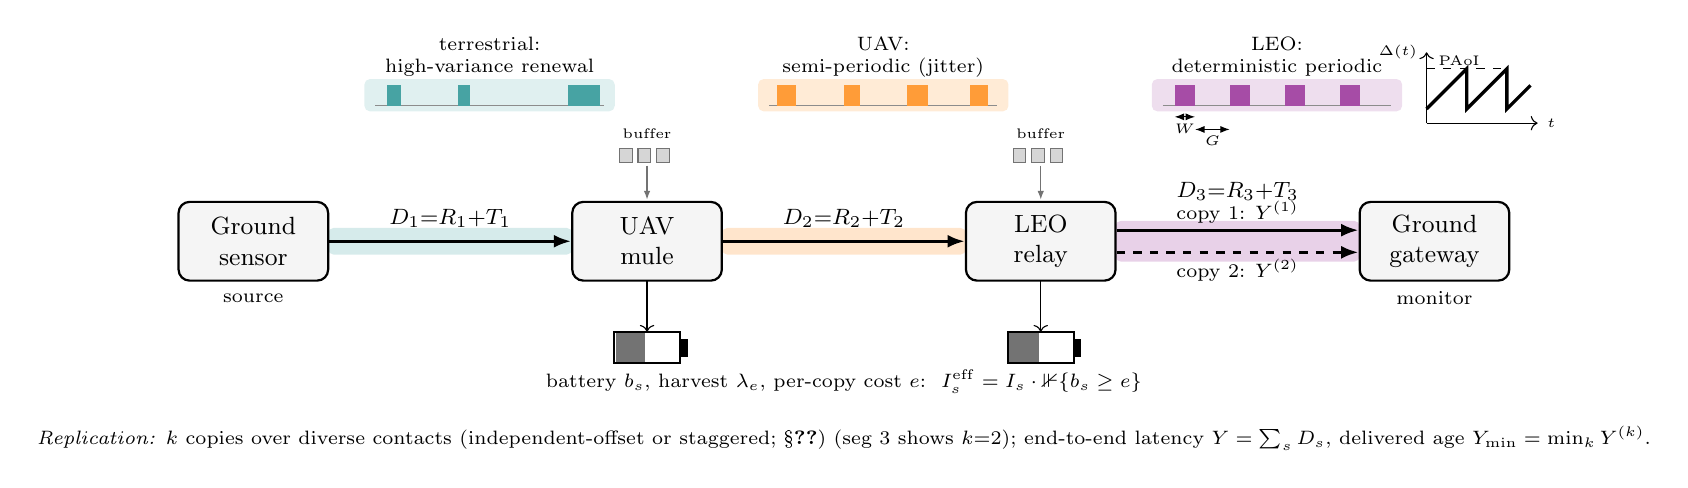
\begin{tikzpicture}[font=\small,
  station/.style={draw,thick,rounded corners,minimum width=1.9cm,
    minimum height=1.0cm,align=center,fill=black!4},
  seg/.style={-{Latex[length=2.2mm]},very thick},
  lbl/.style={font=\footnotesize,align=center}]
\colorlet{cterr}{teal}\colorlet{cuav}{orange}\colorlet{cleo}{violet}

% --- colored bands tie each segment to its contact-model strip ---
\fill[cterr!16,rounded corners=2pt] (0.95,-0.17) rectangle (4.05,0.17);
\fill[cuav!20,rounded corners=2pt]  (5.95,-0.17) rectangle (9.05,0.17);
\fill[cleo!18,rounded corners=2pt]  (10.95,-0.26) rectangle (14.05,0.26);

% --- stations ---
\node[station] (s) at (0,0)   {Ground\\sensor};
\node[station] (u) at (5,0)   {UAV\\mule};
\node[station] (l) at (10,0)  {LEO\\relay};
\node[station] (g) at (15,0)  {Ground\\gateway};
\node[lbl,font=\scriptsize] at (0,-0.72) {source};
\node[lbl,font=\scriptsize] at (15,-0.72) {monitor};

% --- segments 1,2 (single copy) ---
\draw[seg] (s) -- node[lbl,above=1pt]{$D_1{=}R_1{+}T_1$} (u);
\draw[seg] (u) -- node[lbl,above=1pt]{$D_2{=}R_2{+}T_2$} (l);

% --- segment 3 (LEO): two explicit decorrelated copies (k=2) ---
\node[lbl] at (12.5,0.63){$D_3{=}R_3{+}T_3$};
\draw[seg] ([yshift=4pt]l.east) --
  node[lbl,font=\scriptsize,above=-1.5pt]{copy 1: $Y^{(1)}$} ([yshift=4pt]g.west);
\draw[seg,dashed] ([yshift=-4pt]l.east) --
  node[lbl,font=\scriptsize,below=-1.5pt]{copy 2: $Y^{(2)}$} ([yshift=-4pt]g.west);

% --- store-carry-forward buffers at the relays ---
\foreach \x in {5,10}{
  \foreach \i in {0,1,2}{\fill[black!16,draw=black!55]
    ({\x-0.35+0.235*\i},1.0) rectangle ({\x-0.19+0.235*\i},1.18);}
  \node[lbl,font=\tiny] at (\x,1.37){buffer};
  \draw[-{Latex[length=1.1mm]},thin,black!55] (\x,0.96)--(\x,0.53);
}

% --- color-coded ON/OFF schedule strips (contact models) ---
\begin{scope}[shift={(1.55,1.72)}]
  \fill[cterr!12,rounded corners=2pt] (-0.14,-0.07) rectangle (3.04,0.34);
  \draw[thin,black!45] (0,0)--(2.9,0);
  \foreach \a/\b in {0.15/0.32,1.05/1.2,2.45/2.85}{\fill[cterr!72] (\a,0) rectangle (\b,0.26);}
  \node[lbl,font=\scriptsize] at (1.45,0.62){terrestrial:\\high-variance renewal};
\end{scope}
\begin{scope}[shift={(6.55,1.72)}]
  \fill[cuav!16,rounded corners=2pt] (-0.14,-0.07) rectangle (3.04,0.34);
  \draw[thin,black!45] (0,0)--(2.9,0);
  \foreach \a/\b in {0.1/0.34,0.95/1.15,1.75/2.02,2.55/2.78}{\fill[cuav!78] (\a,0) rectangle (\b,0.26);}
  \node[lbl,font=\scriptsize] at (1.45,0.62){UAV:\\semi-periodic (jitter)};
\end{scope}
\begin{scope}[shift={(11.55,1.72)}]
  \fill[cleo!13,rounded corners=2pt] (-0.14,-0.07) rectangle (3.04,0.34);
  \draw[thin,black!45] (0,0)--(2.9,0);
  \foreach \x in {0.15,0.85,1.55,2.25}{\fill[cleo!70] (\x,0) rectangle ({\x+0.26},0.26);}
  \node[lbl,font=\scriptsize] at (1.45,0.62){LEO:\\deterministic periodic};
  \draw[{Latex[length=1.2mm]}-{Latex[length=1.2mm]}] (0.15,-0.14)--(0.41,-0.14);
  \node[font=\tiny,below=-1pt] at (0.28,-0.14){$W$};
  \draw[{Latex[length=1.2mm]}-{Latex[length=1.2mm]}] (0.41,-0.30)--(0.85,-0.30);
  \node[font=\tiny,below=-1pt] at (0.63,-0.30){$G$};
\end{scope}

% --- batteries / energy gate at relays ---
\foreach \x in {5,10}{
  \draw[thick] (\x-0.42,-1.55) rectangle (\x+0.42,-1.15);
  \draw[thick,fill=black] (\x+0.42,-1.45) rectangle (\x+0.5,-1.25);
  \fill[black!55] (\x-0.4,-1.53) rectangle (\x-0.02,-1.17);
  \draw[->,thin] (\x,-0.5)--(\x,-1.15);
}
\node[lbl,font=\scriptsize] at (7.5,-1.78)
  {battery $b_s$, harvest $\lambda_e$, per-copy cost $e$:\ \ $I^{\mathrm{eff}}_s=I_s\cdot\mathbb{1}\{b_s\ge e\}$};

% --- replication note (centred on the chain midpoint x=7.5) ---
\node[lbl,font=\scriptsize,align=center] at (7.5,-2.5)
  {\emph{Replication:} $k$ copies over diverse contacts (independent-offset or staggered; \S\ref{sec:r3}) (seg~3 shows
   $k{=}2$);\ end-to-end latency $Y=\sum_s D_s$, delivered age
   $Y_{\min}=\min_k Y^{(k)}$.};

% --- AoI sawtooth inset at the monitor ---
\begin{scope}[shift={(14.9,1.5)},scale=0.6]
  \draw[->] (0,0)--(2.35,0) node[right,font=\tiny]{$t$};
  \draw[->] (0,0)--(0,1.5) node[left,font=\tiny]{$\Delta(t)$};
  \draw[very thick] (0,0.3)--(0.85,1.15)--(0.85,0.3)--(1.7,1.15)--(1.7,0.3)--(2.2,0.8);
  \draw[dashed,thin] (0,1.15)--(1.7,1.15);
  \node[font=\tiny,anchor=west] at (0.05,1.32){PAoI};
\end{scope}
% balance the bounding box about the chain centre so the diagram is centred
\path (-1.7,0) (16.7,0);
\end{tikzpicture}}
\caption{System model. A status source (ground sensor) reaches the
monitor (ground gateway) over an ordered chain of \emph{scheduled,
intermittently available} segments (terrestrial opportunistic, UAV
mule, LEO relay), each a store-carry-forward server, in which bundles
wait in a buffer, that is ON only during contact windows. The color-coded
per-segment ON/OFF pattern differs by segment type (high-variance renewal,
semi-periodic with jitter, deterministic periodic), so a bundle generated
mid-gap ages for a residual wait $R_s$ before a service+propagation
$T_s$, giving increment $D_s=R_s+T_s$ and end-to-end latency
$Y=\sum_s D_s$. Bundles are \emph{replicated} over $k$ \emph{diverse}
contacts, either with independent offsets or deterministically
staggered; Section~\ref{sec:r3} treats the two regimes separately
(independent offsets give independent residuals, staggered fixed plans
give negatively dependent ones, and distinct router next-hops guarantee
neither). Segment~3 illustrates $k{=}2$ with
copies $Y^{(1)},Y^{(2)}$ and delivered age $Y_{\min}=\min_k Y^{(k)}$. A
finite energy-harvesting battery at each relay gates its usable contacts,
$I^{\mathrm{eff}}_s=I_s\cdot\mathbb{1}\{b_s\ge e\}$.
The monitor tracks the Age of Information $\Delta(t)$ and its peak (PAoI).}
\label{fig:model}
\end{figure*}

A status source delivers updates to a remote monitor over an ordered
chain of $S$ store-carry-forward segments, indexed $s=1,\dots,S$. In the
canonical instance (Fig.~\ref{fig:model}), a ground sensor (the
source) reaches a ground gateway (the monitor) through a UAV mule and a
LEO relay, so the path is ground
sensor~$\to$~UAV~$\to$~LEO~$\to$~ground gateway. Each segment is a server
whose availability is dictated by a contact schedule rather than being
continuous. Table~\ref{tab:notation} collects the notation.

\paragraph*{Per-segment contact abstraction}
\begin{itemize}
\item \emph{LEO}: deterministic periodic ON/OFF, window $W_s$ once per
period $P_s$ (Section~\ref{sec:r1});
\item \emph{UAV}: semi-periodic / jittered renewal ON/OFF (reduces to
the LEO case as jitter $\to 0$; genuinely Markov-modulated schedules,
with correlated successive gaps, are an extension);
\item \emph{Terrestrial}: stochastic renewal ON/OFF.
\end{itemize}

\paragraph*{Quantities and the freshness metrics}
$\AoI(t)=t-g^{\star}(t)$ is the AoI at the monitor, where $g^{\star}(t)$
is the generation time of the freshest \emph{delivered} bundle; it drifts
up at unit rate and resets whenever a delivery brings fresher
information (a stale or duplicate copy causes no reset). Intermittent
gating supports two distinct traffic models with different peak-age
processes, so we define \emph{three} peak quantities and state, for
every result, which one it characterizes (Fig.~\ref{fig:metric}):
\begin{itemize}
\item \emph{per-reset} $\PAoI$ (textbook): the average of the age just
before \emph{every} reset. When a window delivers a back-to-back burst
of updates it also counts the small intra-burst peaks, deflating the
average;
\item \emph{outage-peak age} $\OPAoI$: the average, over contact
cycles, of the maximum age just before that contact's deliveries, that
is, the worst-case staleness per silent gap. Under \emph{generate-at-will}
traffic (fresh data available at every window) the single-LEO cycle
peak is $\OPAoI=T_s+G$ (Section~\ref{sec:r1});
\item \emph{per-update} $\PAoIper$: the standard PAoI when the source
launches one update per firing epoch (paced generation): each update
yields one reset, and $\E[\PAoIper]=\E[Z]+\E[\Ymin]$ with $Z$ the
inter-firing interval and $\Ymin$ the delivered latency. Here per-reset
and per-update coincide. The identity presumes that deliveries
\emph{preserve generation order}: if a newer update overtakes an older
one, the older delivery arrives stale and resets nothing. Order
preservation is guaranteed when the latency spread is bounded by the
firing interval, $Y_{\max}-Y_{\min}\le Z_{\min}$, which is checkable
from the plan for lattice-supported $Z$ and bounded $Y$; on long
multi-segment paths $\sum_s G_s$ can exceed the firing interval, and the
condition then binds. When order preservation fails, $\PAoIper$ must be
evaluated over the subsequence of \emph{freshness-resetting}
deliveries, and $\E[Z]+\E[\Ymin]$ then neither characterizes nor
bounds that process: consecutive resets can sit several firing
intervals apart while the resetting updates are the atypically fast
ones, so the true peak can land on either side. For example,
deterministic $Z{=}1$ with repeating latencies $4,3,2,0,5$ resets once
per five epochs with peak $5>\E[Z]{+}\E[Y]{=}3.8$.
\end{itemize}
These are genuinely different processes: for $P{=}1$, $W{=}0.1$, and
$T_s{\approx}0$, $\OPAoI=0.9$ while $\E[\PAoIper]=P+\E[R]=1.405$, and
neither approximates the other.
Result~1 and the renewal generalization characterize $\OPAoI$ (and
time-average AoI); Results~2--3, the tail corollary, and the policy
characterize $\PAoIper$ under paced generation. Our protocol-level
(Tier-2) reconstruction clusters resets within one contact window and
keeps the burst maximum, so it measures $\OPAoI$
(Section~\ref{sec:sim}); the model-exact (Tier-1) simulations of
Result~3 measure $\PAoIper$. For a single copy, the per-segment latency
increment is $D_s=R_s+T_s$ with $R_s$ the residual wait and $T_s$ the
lumped (near-deterministic) service plus propagation, and the end-to-end
latency is $Y=\sum_{s=1}^S D_s$; with replication degree $k$ the delivered
latency is $\Ymin=\min(Y^{(1)},\dots,Y^{(k)})$. Throughout,
``closed-form'' means an explicit expression under the assumptions
stated with the result: random schedule offsets
(Section~\ref{sec:r2}), order-preserving deliveries, and, for the
threshold's fluid form, a large battery. Each result names the
assumption that carries its form. Table~\ref{tab:assumptions} lists
these assumptions with the consequence of violating each.

\paragraph*{Traffic model: fixed sampling cadence (modeling choice)}
Under paced generation the source emits one update per firing epoch,
and throughout Sections~\ref{sec:r3}--\ref{sec:policy} the firing epochs
recur once per contact period $P$ of the gating bottleneck (so
$\E[Z]=P$ when every epoch fires). The \emph{sampling cadence is held
fixed and the energy budget is spent on copies only}. This is a
deliberate modeling choice, and we state what it covers. (i)
\emph{Application-paced sampling:} the instant at which an update
exists is set by the application (a measurement cycle, an event
report), not by the transport, so the source can neither defer
sampling to a window opening nor replace the sample by a fresher one
later. (ii)
\emph{Downstream bottlenecks:} a relay cannot resample the bundle it
holds, so against the residual at a gating bottleneck beyond the source
the only lever is the number of distinct contacts the update rides,
i.e.\ the copy degree. (iii) The per-update peak $\PAoIper=Z+\Ymin$
separates the two levers exactly: the cadence $Z$ is the sampling
decision and the delivered latency $\Ymin$ the copy decision, so fixing
$Z$ isolates the question this paper asks. The choice also excludes a
case, which we concede: a source that can sample at will, and whose
routes diverge at the source, does at least as well by placing a
\emph{fresh} sample on each route at that route's own contact as by
copying one sample, at the same energy. That is the generate-at-will
regime of Section~\ref{sec:r1} applied to the union of the routes'
schedules, and replication in our sense then has nothing to add at the
source. A joint allocation of one budget between sampling rate and copy
degree is a natural generalization that we do not treat;
Proposition~\ref{prop:uncertain} shows how replication nevertheless acts
on the realized inter-\emph{delivery} cadence once route outcomes are
uncertain.

The firing epoch is \emph{exogenous to the plan}: its phase relative to
each route's schedule is set by the application, not chosen by the
source, and is modeled as uniformly distributed. The degree set-point
is computed without conditioning on it, although per-bundle placement
may use it (Section~\ref{sec:policy}). The even-stagger profile and the
tail of Corollary~\ref{cor:tail} are averages over that phase on the
stated plan. The phase-agnostic profile $g_k$ is in addition an average
over route offsets; on one fixed plan it is a time average only when
the route periods are pairwise incommensurate (plan model~(i) of
Section~\ref{sec:r3}), and on a co-period plan the realized value is the
plan's joint-survival integral \eqref{eq:rminjoint}, which can lie
anywhere on the phase ladder \eqref{eq:ladder}.

\paragraph*{Uncongested-contact regime (scope)}
Throughout, a contact is usable the instant it opens and $T_s$ absorbs
transmission and propagation: we work in the \emph{low-load} regime
where contact capacity (window duration $\times$ rate) exceeds the
offered bundle volume. Residual waits (hours) then dominate service
times (seconds), and replication's second cost, \emph{contact volume},
is negligible next to its energy cost. Status updates sit deep in this
regime (our Iridium scenario uses ${\sim}10^{-5}$ of a window per
update), but the assumption is load-bearing: near contact capacity,
in-window queueing, overbooking~\cite{bezirgiannidis}, and the volume
of extra copies re-enter. Section~\ref{sec:sim} measures the boundary.

\begin{figure}[t]
\centering
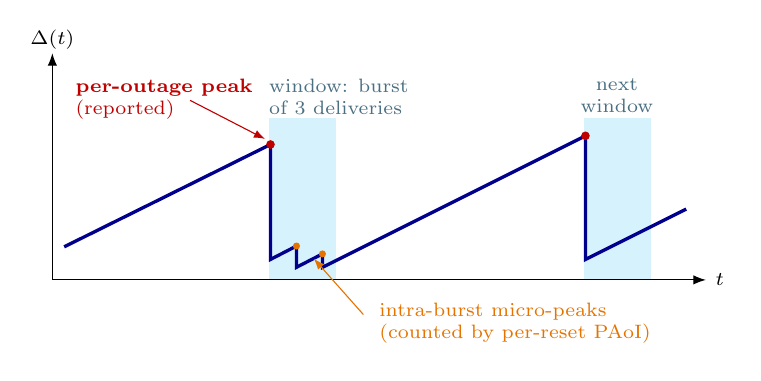
\begin{tikzpicture}[font=\footnotesize,x=1cm,y=1cm,
  note/.style={font=\scriptsize,align=center}]
\colorlet{cwin}{cyan!16}\colorlet{cage}{blue!55!black}
\colorlet{cpk}{red!75!black}\colorlet{cmicro}{orange!90!black}
% contact windows (shaded)
\fill[cwin] (2.6,0) rectangle (3.45,2.05);
\fill[cwin] (6.6,0) rectangle (7.45,2.05);
\node[note,cyan!45!black,anchor=north west,align=left] at (2.48,2.68)
  {window: burst\\of 3 deliveries};
\node[note,cyan!45!black,anchor=north] at (7.02,2.68) {next\\window};
% axes
\draw[-{Latex[length=1.6mm]}] (-0.15,0)--(8.15,0) node[right,font=\scriptsize]{$t$};
\draw[-{Latex[length=1.6mm]}] (-0.15,0)--(-0.15,2.88)
  node[above,font=\scriptsize,inner sep=1pt]{$\AoI(t)$};
% sawtooth: gap ramp, burst of 3 resets in window, gap ramp, reset
\draw[very thick,cage]
 (0,0.42)--(2.62,1.72)--(2.62,0.26)--(2.95,0.43)--(2.95,0.16)
 --(3.28,0.33)--(3.28,0.16)--(6.62,1.83)--(6.62,0.26)--(7.9,0.9);
% outage peaks (dots + label placed in the free upper-left area)
\fill[cpk] (2.62,1.72) circle (0.055);
\fill[cpk] (6.62,1.83) circle (0.055);
\node[note,cpk,anchor=north west,align=left] at (0.02,2.68)
  {\textbf{per-outage peak}\\(reported)};
\draw[-{Latex[length=1.4mm]},cpk] (1.60,2.28) -- (2.55,1.79);
% micro peaks annotated below the axis (keeps the curve clear)
\fill[cmicro] (2.95,0.43) circle (0.045);
\fill[cmicro] (3.28,0.33) circle (0.045);
\draw[-{Latex[length=1.4mm]},cmicro] (3.80,-0.44) -- (3.17,0.27);
\node[note,cmicro,anchor=west,align=left] at (3.88,-0.55)
  {intra-burst micro-peaks\\(counted by per-reset PAoI)};
\end{tikzpicture}
\caption{The peak-age taxonomy. A contact window delivers a back-to-back
burst of distinct updates; each fresher delivery resets the age. The
textbook \emph{per-reset} $\PAoI$ also averages the small intra-burst
peaks, deflating the mean; the \emph{outage peak} $\OPAoI$ keeps only
the burst maximum, the conservative cycle-level statistic (within
each cycle it dominates every intra-burst peak; with variable burst
sizes the two \emph{averages} need not order). Under paced
generation (one update per firing epoch) each update yields one reset
and the per-update peak $\PAoIper=Z+\Ymin$ applies; the three coincide
when each contact delivers exactly one update.}
\label{fig:metric}
\end{figure}

\paragraph*{Energy coupling}
Segment $s$ has a battery level $b_s(t)$, a harvest rate
$\lambda_{e,s}$, and a per-copy energy cost $e$. Its effective
availability is $I^{\mathrm{eff}}_s(t)=I_s(t)\cdot
\ind\{b_s(t)\ge e\}$: energy scarcity thins contacts (stretches the
residual wait) and replication draws the battery down faster (starving
future contacts). This tension is resolved in
Sections~\ref{sec:r3}--\ref{sec:r3hard}. \emph{Scope:} although the
model admits a battery per segment, the threshold analysis of
Sections~\ref{sec:r3}--\ref{sec:r3hard} adopts a \emph{single
energy-bottleneck abstraction}: one battery, at the source or the
tightest node, gates copy launches at a constant per-copy cost $e$; this
is the binding constraint in our scenarios. Route-dependent costs and
interacting per-relay batteries are an extension we do not claim
(Section~\ref{sec:sim} gates energy at the source accordingly).

\paragraph*{Reference scenarios}
Three instances recur in the validation (Section~\ref{sec:sim}) and
are fixed here. \emph{S1, single LEO segment:} Iridium-class period
$P{=}5736$\,s, window $W{=}430$\,s ($\delta{=}0.075$), $T_s{=}10$\,s;
normalized Tier-1 sweeps use $P{=}1$ with $\delta\in\{0.10,0.15\}$.
\emph{S2, relay diamond:} a source reaching one gateway through two or
three bent-pipe relay routes. In the atomic and unified experiments
three relays share the S1 schedule with phases staggered by $P/3$; in
the two-relay experiment of Section~\ref{sec:sim} the relays have
incommensurate pass periods ($5736$\,s and $4500$\,s, windows $430$\,s
and $338$\,s). Relays fail and recover independently with exponential
holding times of mean $8000$\,s (up) and $4000$\,s (down), so each is
down $1/3$ of the time; a fault is \emph{stall-type}: a down relay does
not forward, and no bundle is destroyed. A single source battery gates
launches: the Tier-1 harness uses Poisson harvest with mean $\eta$
copies per period and $B{=}12$, whereas the Tier-2 energy module
harvests at a constant rate into a battery of five, six, or $32$ copies
(stated per experiment). \emph{S3,
heterogeneous chain:} sensor~$\to$~UAV mule~$\to$~LEO~$\to$~gateway with
gamma-distributed terrestrial gaps (mean $3000$\,s, window $300$\,s,
coefficient of variation $\mathrm{CV}{=}1.3$), a UAV segment periodic with Gaussian jitter
($P{=}1800$\,s, $W{=}180$\,s, jitter standard deviation $240$\,s), the
S1 LEO segment, and one update every $\GEN{=}400$\,s.

\begin{remark}[Report both metrics]
Exact average AoI in tandems is closed-form only to two--three hops,
while the peak metrics remain reachable; and under intermittency
$\OPAoI$ can fall \emph{below} time-average AoI
(Remark~\ref{rem:inversion}), so we report peak and average
throughout.
\end{remark}

\begin{table}[t]
\caption{Notation.}
\label{tab:notation}
\centering
\renewcommand{\arraystretch}{1.12}
\setlength{\tabcolsep}{4pt}
\footnotesize
\begin{tabular}{ll}
\hline
$P,\,W,\,G$ & contact period, window, silent gap $G=P-W$ \\
$\delta$ & duty cycle $W/P$;\; $\dutyeff=\delta\peff$ usable-ON fraction \\
$U$ & arrival phase (Sec.~\ref{sec:r1}); ON duration (Sec.~\ref{sec:renewal}) \\
$V,\,C$ & OFF gap, renewal cycle $C=U+V$ (Sec.~\ref{sec:renewal}) \\
$R_s,\,T_s$ & residual wait; service$+$propagation at segment $s$ \\
$D_s,\,Y$ & increment $R_s{+}T_s$; end-to-end latency $\sum_s D_s$ \\
$k,\,\Ymin$ & replication degree; delivered latency $\min_k Y^{(k)}$ \\
$Z,\,\AoI$ & inter-firing interval; age at the monitor \\
$\OPAoI,\,\PAoIper$ & outage-peak age; per-update peak age \\
$b_s,\,B,\,e$ & battery level, capacity, per-copy energy cost \\
$\lambda_e,\,\eta$ & harvest rate; energy adequacy $\lambda_e P/e$ \\
$\peff,\,L$ & usable-window probability; cap-overflow loss \\
$\mathcal{A}(k),\,\kstar$ & mean-$\PAoIper$ objective \eqref{eq:obj}; optimal degree \\
$K_{\max}$ & candidate copy routes / contact opportunities \\
\hline
\end{tabular}
\end{table}

\begin{table}[t]
\caption{Modeling assumptions and their failure modes.}
\label{tab:assumptions}
\centering
\renewcommand{\arraystretch}{1.2}
\begin{tabular}{p{2.5cm}p{1.1cm}p{3.3cm}}
\hline
Assumption & Where & If violated \\
\hline
Decorrelated contacts per copy & Results 2--3 & same-bottleneck copies: gain $\to 0$ \\
Random offsets / spread-out delays & Sec.~\ref{sec:r2}, Rem.~\ref{rem:fixedmix} & commensurate or lattice: locking \\
$k\le 2$ closed form & Result 2 & general $k$ via $\int(1-F_Y)^k$ (numerical) \\
Generate-at-will & Result 1 & finite $\lambda$: $+1/\lambda$ floor (Sec.~\ref{sec:renewal}) \\
Large battery & Result 3 (fluid $\peff$) & finite $B$: $\peff\le\min(1,\eta/k)$; below $B^{\dagger}(\eta)$ (Sec.~\ref{sec:policy}) the optimum is lower \\
\hline
\end{tabular}
\end{table}

% =====================================================================
\section{Result 1: Residual-Wait Laws for Scheduled
Contacts}\label{sec:r1}
A LEO satellite rises over the ground terminal once per orbital period
$P$ and stays in view for a contact window of duration $W$; the link is
therefore ON during $[0,W)$ of each period and OFF (dark) during the
silent gap $G\triangleq P-W$ that follows, so the terminal is in contact
only a fraction $\delta\triangleq W/P$ of the time, the duty cycle
(Fig.~\ref{fig:r1def}). A status update generated at a stationary
(random-phase) instant meets this schedule at a uniformly random phase $U\sim\mathrm{Unif}[0,P)$
(justified by the random-offset mixing property of
Section~\ref{sec:r2}): if $U$ falls inside a window the
bundle is forwarded at once, otherwise it must age in buffer until the
next pass. This residual wait is
\begin{equation}
R=\begin{cases}0,& U\in[0,W)\\ P-U,& U\in[W,P)\end{cases},
\end{equation}
a mixed law with atom $\Prob(R=0)=W/P$ and uniform slab $f_R(r)=1/P$ on
$(0,G]$; $\Prob(R>r)=(G-r)/P$ on $[0,G]$, $R_{\max}=G$.

\begin{figure}[t]
\centering
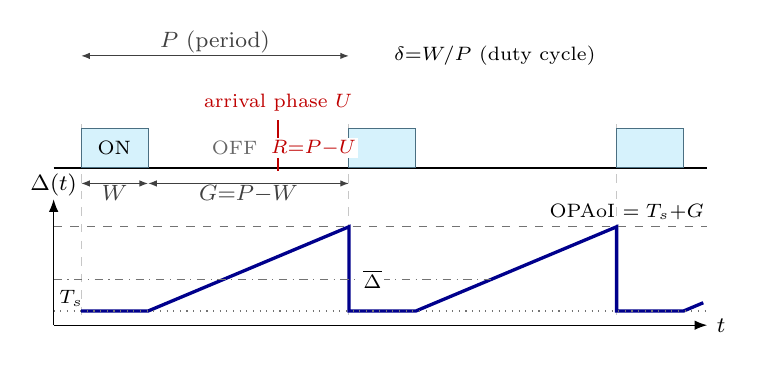
\begin{tikzpicture}[font=\footnotesize,x=1cm,y=1cm,
  win/.style={fill=cyan!16,draw=cyan!45!black,thin},
  ax/.style={-{Latex[length=1.6mm]}},
  dim/.style={{Latex[length=1.1mm]}-{Latex[length=1.1mm]},black!75}]
\colorlet{cage}{blue!55!black}\colorlet{carr}{red!75!black}
% vertical guides at window openings (link schedule to AoI)
\foreach \x in {0,3.4,6.8}{\draw[dashed,black!22] (\x,2.55)--(\x,0.02);}
% ===== schedule panel (link ON/OFF) =====
\draw[thick] (-0.35,2.0)--(7.95,2.0);
\foreach \x in {0,3.4,6.8}{\fill[win] (\x,2.0) rectangle (\x+0.85,2.5);}
\node[font=\scriptsize] at (0.42,2.25){ON};
\node[font=\scriptsize,black!60] at (1.95,2.25){OFF};
% period / duty-cycle dimensions raised clear of the arrival annotation
\draw[dim] (0,3.42)--(3.4,3.42) node[midway,above,inner sep=1pt]{$P$ (period)};
\node[font=\scriptsize,anchor=west] at (3.85,3.42){$\delta{=}W/P$ (duty cycle)};
% W and G on one line beneath the bar
\draw[dim] (0,1.80)--(0.85,1.80) node[midway,below,inner sep=0.5pt]{$W$};
\draw[dim] (0.85,1.80)--(3.4,1.80) node[midway,below,inner sep=0.5pt]{$G{=}P{-}W$};
% arrival + residual wait
\draw[thick,carr] (2.5,1.96)--(2.5,2.60);
\node[font=\scriptsize,carr,anchor=south,inner sep=1.5pt] at (2.5,2.66){arrival phase $U$};
\draw[dim,carr] (2.5,2.25)--(3.4,2.25);
\node[font=\scriptsize,carr,fill=white,inner sep=0.8pt] at (2.95,2.25){$R{=}P{-}U$};
% ===== AoI panel: sawtooth Delta(t) =====
\draw[ax] (-0.35,0)--(7.95,0) node[right]{$t$};
\draw[ax] (-0.35,0)--(-0.35,1.60) node[above,inner sep=1pt]{$\Delta(t)$};
\draw[very thick,cage]
  (0,0.18)--(0.85,0.18)--(3.4,1.25)--(3.4,0.18)--(4.25,0.18)--(6.8,1.25)
  --(6.8,0.18)--(7.65,0.18)--(7.9,0.285);
\draw[dashed,black!55] (-0.35,1.25)--(7.95,1.25);
\node[font=\scriptsize,anchor=east,inner sep=1pt] at (7.95,1.44){OPAoI $=T_s{+}G$};
\draw[dashdotted,black!55] (-0.35,0.58)--(5.2,0.58);
\node[font=\scriptsize,anchor=west,fill=white,inner sep=0.8pt] at (3.55,0.58){$\overline{\Delta}$};
\draw[dotted,black!55] (-0.35,0.18)--(7.95,0.18);
\node[font=\scriptsize,anchor=west,inner sep=1pt] at (-0.32,0.34){$T_s$};
\end{tikzpicture}
\caption{Result~1 parameters. \emph{Top:} the LEO segment is ON for a
window $W$ once per period $P$ (silent gap $G{=}P{-}W$, duty cycle
$\delta{=}W/P$); a bundle generated at arrival phase $U$ in the gap waits
a residual $R{=}P{-}U$ for the next window. \emph{Bottom:} the resulting
age $\Delta(t)$ is pinned near the service+propagation floor $T_s$ during
a window and ramps over the gap, peaking at $\OPAoI{=}T_s{+}G$; the
time-average is $\overline{\Delta}{=}T_s{+}(P{-}W)^2/2P$
(Theorem~\ref{thm:r1}).}
\label{fig:r1def}
\end{figure}

\begin{theorem}[LEO AoI/OPAoI anchor]\label{thm:r1}
With service$+$propagation $T_s$,
\begin{align}
\E[R]&=\frac{(P-W)^2}{2P}=\tfrac{P}{2}(1-\delta)^2,\quad
\E[R^2]=\frac{G^3}{3P},\\
\overline{\AoI}_{\mathrm{LEO}}&=T_s+\tfrac{P}{2}(1-\delta)^2,\qquad
\OPAoI_{\mathrm{LEO}}=T_s+P(1-\delta).
\end{align}
\end{theorem}
The law itself is classical residual-life theory, stated as the anchor
on which the DTN-specific structure builds. Note the provisioning
consequence: sparse contacts hurt the mean age \emph{quadratically} in
$(1-\delta)$ but the peak only \emph{linearly}, so mean- and
peak-optimal contact provisioning differ. Fig.~\ref{fig:r1} checks both
forms against simulation (E1--E2); the fitted exponents of $(1-\delta)$
are $1.98$ for the mean and $1.00$ for the peak.

% AUTO-GENERATED by figs/make_figures.py -- do not edit.
\begin{figure}[t]\centering
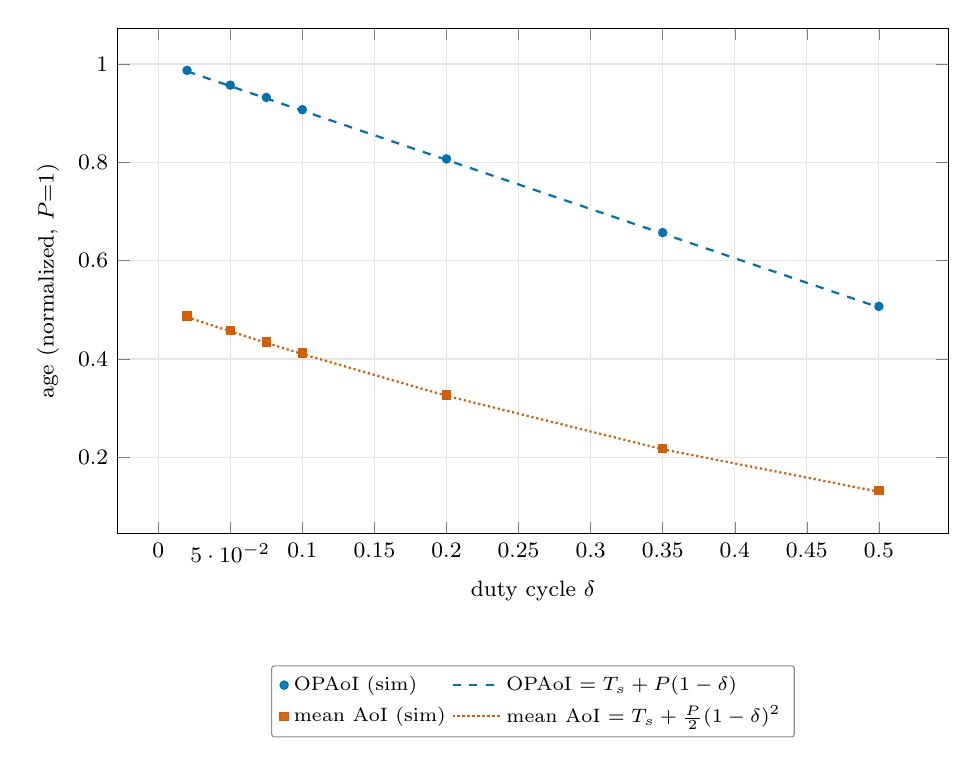
\begin{tikzpicture}
\begin{axis}[paperfig,width=\columnwidth,height=0.66\columnwidth,
  xlabel={duty cycle $\delta$},ylabel={age (normalized, $P{=}1$)},
  legend style={at={(0.5,-0.26)},anchor=north,legend columns=2},
  error bars/y dir=both,error bars/y explicit]
\addplot[cA,only marks,mark=*,mark size=1.5pt] coordinates {(0.02,0.9870100715269062) +- (0,3.1292142984718735e-05) (0.05,0.9569975439410504) +- (0,2.8138476284065702e-05) (0.075,0.9320010411719328) +- (0,2.902494335842732e-05) (0.1,0.9069955973162998) +- (0,1.893193054617168e-05) (0.2,0.8069971556041535) +- (0,2.4082530275375084e-05) (0.35,0.657020357263457) +- (0,2.364619973598577e-05) (0.5,0.5069971053296146) +- (0,2.473059005205108e-05)};
\addlegendentry{OPAoI (sim)}
\addplot[cA,no marks,thick,dashed] coordinates {(0.02,0.985) (0.05,0.955) (0.075,0.93) (0.1,0.905) (0.2,0.805) (0.35,0.655) (0.5,0.505)};
\addlegendentry{OPAoI $=T_s+P(1-\delta)$}
\addplot[cB,only marks,mark=square*,mark size=1.5pt] coordinates {(0.02,0.48721054412512643) +- (0,3.05966842493133e-05) (0.05,0.45824685360113504) +- (0,2.693793306118609e-05) (0.075,0.4348135198357405) +- (0,2.655059400816846e-05) (0.1,0.4119961987610867) +- (0,1.6638518202369598e-05) (0.2,0.3269977862109709) +- (0,1.944432796664332e-05) (0.35,0.21826373712641028) +- (0,1.6032026469115834e-05) (0.5,0.13199933546467407) +- (0,1.2466013684464939e-05)};
\addlegendentry{mean AoI (sim)}
\addplot[cB,no marks,thick,densely dotted] coordinates {(0.02,0.48519999999999996) (0.05,0.45625) (0.075,0.43281250000000004) (0.1,0.41000000000000003) (0.2,0.32500000000000007) (0.35,0.21625000000000003) (0.5,0.13)};
\addlegendentry{mean AoI $=T_s+\tfrac{P}{2}(1-\delta)^2$}
\end{axis}
\end{tikzpicture}
\caption{Result~1 (E1/E2): simulated mean AoI and OPAoI vs.\ duty cycle
match the closed forms; the peak grows linearly and the mean
quadratically in $(1-\delta)$ (provisioning divergence). Markers are
Monte Carlo means with 95\% confidence intervals (smaller than
markers).}
\label{fig:r1}
\end{figure}


\paragraph*{Energy-thinning bridge}
If each window is usable with probability $\peff$ (battery $\ge e$),
i.i.d.\ across periods, the usable schedule is again alternating-renewal
with OFF gap $V'=(J{-}1)P+G$, $J\sim\mathrm{Geom}(\peff)$, so every
closed form extends through the renewal law of
Section~\ref{sec:renewal} with $V\to V'$; in particular the exact
thinned residual is
\begin{equation}\label{eq:thin}
\E[R_{\mathrm{eff}}]=
\underbrace{\frac{(P-W)^2}{2P}}_{\text{contact gating}}
+\underbrace{P\,\frac{1-\peff}{\peff}}_{\text{energy thinning}}
-\underbrace{\frac{(1-\peff)W^2}{2P}}_{O(\delta^2)} .
\end{equation}
(Derivation: with $J\sim\mathrm{Geom}(\peff)$, $\E[V']=P/\peff-W$ and
$\E[C']=P/\peff$, while
$\E[V'^2]=P^2(1-\peff)(2-\peff)/\peff^2+2PG(1-\peff)/\peff+G^2$;
substituting into $\E[R]=\E[V'^2]/2\E[C']$ and writing $G=P-W$ gives
\eqref{eq:thin}, whose last term, the $O(\delta^2)$ correction,
collects the $W^2$ contributions that arise because a skipped period
adds a whole $P$, not a gap $G$, to the silence.)
We caution that this is a \emph{thinning}, not a rescaling: the
shorthand $\dutyeff=\delta\peff$ preserves only the long-run usable-ON
fraction, and substituting $\delta\mapsto\delta\peff$ into the
Theorem~\ref{thm:r1} forms does \emph{not} reproduce
\eqref{eq:thin}. Skipped windows cluster the silence into whole
periods, which the residual's second-moment dependence
($\E[V'^2]/2\E[C']$) captures and a duty-cycle rescaling does not. The
i.i.d.\ premise itself is a mean-field approximation, because a finite
battery correlates consecutive windows; Section~\ref{sec:r3hard} makes
this precise.

% =====================================================================
\subsection{Renewal Generalization: UAV and Terrestrial
Segments}\label{sec:renewal}
Real UAV and terrestrial links are not perfectly periodic: a UAV mule
revisits the sensor field on a jittered patrol, and opportunistic
terrestrial contacts appear at random. One \emph{alternating-renewal}
model captures all three segment types, with the deterministic LEO
schedule as a special case, by letting each contact cycle be an ON
period of duration $U$ (the window) followed by an OFF gap of duration
$V$ (mean $G$, the dark interval before the next contact), where $U$ and
$V$ may now be random; the cycle length is $C=U+V$ and the duty cycle is
$\delta=\mathbb E[U]/\mathbb E[C]$. By renewal-reward and the inspection
paradox, a stationary arrival sees
\begin{equation}\label{eq:renewal}
\begin{aligned}
\Pr(R{=}0)&=\delta,\qquad f_R(r)=\frac{\Pr(V>r)}{\mathbb E[C]},\\
\E[R]&=\frac{\E[V^2]}{2\,\E[C]},\qquad \E[\OPAoI]=T_s+\E[V].
\end{aligned}
\end{equation}
Deterministic $V$ recovers Theorem~\ref{thm:r1} (LEO); a low-variance $V$
models UAV semi-periodic jitter (and tends to LEO as the jitter
vanishes); exponential $V$ gives the two-state continuous-time Markov
chain of an unreliable server, here a special case rather than the
contribution; and high-variance or heavy-tailed $V$ models opportunistic
terrestrial contacts. The identities \eqref{eq:renewal}
need only a stationary, ergodic ON/OFF sequence (they follow by Palm
inversion), not independence of successive cycles, so they also cover
the jittered-periodic UAV schedule of scenario S3, whose successive gaps
share a jitter term.

\begin{remark}[AoI/PAoI inversion]\label{rem:inversion}
Mean $\OPAoI$ depends only on $\E[V]$ while mean AoI grows with the gap
variance, so
$\E[\OPAoI]<\overline{\AoI}\iff \E[V^2]>2\E[C]\E[V]$. Writing
$C=U+V$, this is exactly
\begin{equation}\label{eq:invcond}
\mathrm{CV}^2(V)>1+\frac{2\,\E[U]}{\E[V]},
\end{equation}
(the algebra: $\E[V^2]>2\E[C]\E[V]$ with $\E[C]=\E[U]+\E[V]$ reads
$\operatorname{Var}V+\E[V]^2>2\E[V]^2+2\E[U]\E[V]$, i.e.\
$\operatorname{Var}V/\E[V]^2>1+2\E[U]/\E[V]$),
which reduces to the familiar $\mathrm{CV}^2(V)>1$ only in the sparse-duty
limit $\delta\to0$ ($\E[U]/\E[V]\to0$); for the plotted parameters
($\E[U]/\E[V]=1/9$) the threshold is $\mathrm{CV}^2\approx1.22$, i.e.\
$\mathrm{CV}\approx1.11$. Peak age can therefore sit
\emph{below} average age on high-variance terrestrial links
(Fig.~\ref{fig:inversion}), so a single freshness number misleads
across heterogeneous segments. The order-statistic replication analysis
below acts on the residual law abstractly; the energy-threshold
structure extends whenever the resulting gain profile and firing
process satisfy the conditions of Section~\ref{sec:r3}.
\end{remark}

% AUTO-GENERATED by figs/make_figures.py -- do not edit.
\begin{figure}[t]\centering
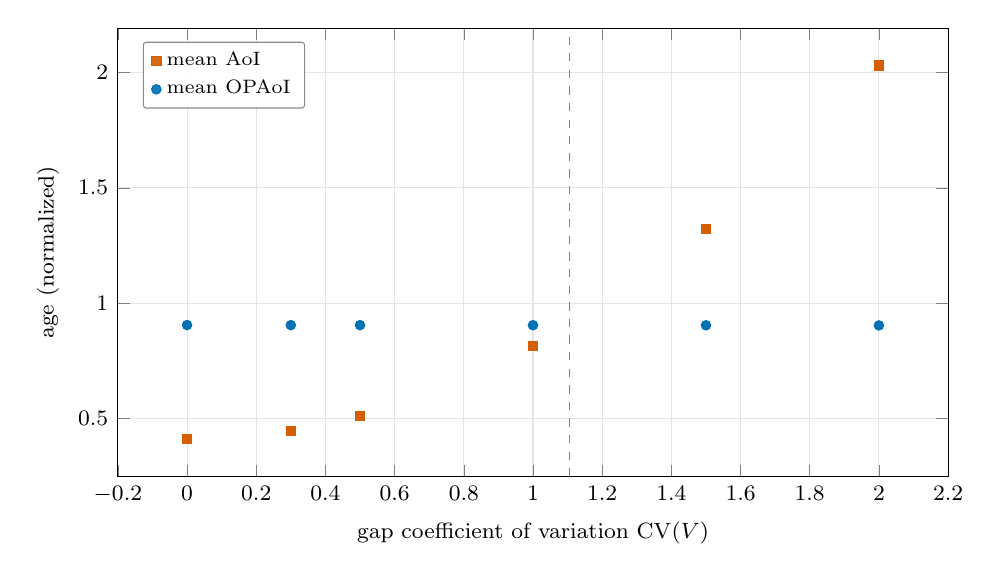
\begin{tikzpicture}
\begin{axis}[paperfig,width=\columnwidth,height=0.6\columnwidth,
  xlabel={gap coefficient of variation $\mathrm{CV}(V)$},
  ylabel={age (normalized)},legend pos=north west,grid=both,
  legend cell align=left]
\addplot[cB,only marks,mark=square*,mark size=1.7pt] coordinates {(0.0,0.41) (0.3,0.44625348238863416) (0.5,0.5108772600771613) (1.0,0.8149996897795648) (1.5,1.3224004704089134) (2.0,2.030147837685105)};
\addlegendentry{mean AoI}
\addplot[cA,only marks,mark=*,mark size=1.7pt] coordinates {(0.0,0.9049999999999999) (0.3,0.9046423617422175) (0.5,0.9044223082534586) (1.0,0.9043348492407165) (1.5,0.9039569330472569) (2.0,0.9033825094312596)};
\addlegendentry{mean OPAoI}
\draw[gray,dashed] (axis cs:1.106,\pgfkeysvalueof{/pgfplots/ymin}) -- (axis cs:1.106,\pgfkeysvalueof{/pgfplots/ymax});
\end{axis}
\end{tikzpicture}
\caption{The AoI/OPAoI inversion (E12). Mean OPAoI ($=T_s+
\mathbb{E}[V]$) is flat in the gap variability, while mean AoI grows
with it; they cross at the exact threshold
$\mathrm{CV}^2(V)=1+2\mathbb{E}[U]/\mathbb{E}[V]$ (dashed:
$\mathrm{CV}\approx1.11$ for the plotted $\mathbb{E}[U]/\mathbb{E}[V]=1/9$),
so for high-variance
terrestrial contacts the outage peak sits {\itshape below}
average AoI.}
\label{fig:inversion}
\end{figure}


% =====================================================================
\section{Result 2: Phase Mixing and Two-Copy PAoI}\label{sec:r2}
Composing segments needs care. The residual wait $R_s$ a bundle incurs at
segment $s$ depends on \emph{when} it reaches that segment relative to the
segment's own schedule, that is, on its arrival phase, which is itself
displaced by all the upstream delays. Writing the phase as
$\Phi_s=\bigl(g+\sum_{j<s}D_j\bigr)\bmod P_s$ (generation time $g$ plus the
accumulated increments, reduced modulo the segment period $P_s$), $R_s$ is
therefore not automatically independent of the upstream increments
$\{D_j\}_{j<s}$, and the per-segment delays cannot simply be added. The
next paragraph gives the condition under which they can.

\paragraph*{Random-offset ensemble: exact phase mixing}
Let each segment's schedule carry an offset
$\Theta_s\sim\mathrm{Unif}[0,P_s)$, independent across segments and of
the generation process (the \emph{random-offset ensemble}). Then
$\Phi_s=(g+\sum_{j<s}D_j-\Theta_s)\bmod P_s$, and conditioning on the
generation time and all upstream increments, the wrap of the independent
uniform $\Theta_s$ is uniform on $[0,P_s)$ and independent of the
conditioning variables and of the other $\Theta_j$ (translation
invariance of the uniform law on the circle). Hence the phases
$\{\Phi_s\}$ are exactly uniform and mutually independent, $\{D_s\}$ are
independent, the aged-update correction vanishes, and
$f_Y=f_{D_1}\ast\cdots\ast f_{D_S}$. We call this the
\emph{random-offset mixing property}; it is the exact statement, and the
fixed-plan case below is an approximation to it.

\begin{remark}[Fixed plans: two asymptotic mechanisms, one
approximation]\label{rem:fixedmix}
For one \emph{fixed} plan (deterministic offsets), uniformity and
independence are not automatic. They arise in two limits.

(a)~\emph{Horizon limit (Weyl).} Under paced generation at spacing
$\GEN$ with $\GEN/P_1$ irrational, the \emph{first-segment} phase
sequence $n\,\GEN\bmod P_1$ equidistributes as the number of updates
grows. This is rigorous, and it justifies the uniform-arrival marginal
on the entry segment of a fixed plan. The error is quantifiable: for a
phase statistic $f$ of bounded total variation $\mathrm{TV}(f)$,
Koksma's inequality gives
$|N^{-1}\sum_{n\le N}f(\Phi_n)-\int f|\le \mathrm{TV}(f)\,D_N^{*}$, where
the star discrepancy $D_N^{*}$ of $\{n\,\GEN/P_1\}$ is
$O(N^{-1}\log N)$ when $\GEN/P_1$ has bounded partial
quotients~\cite{kuipers1974}. For the residual, $\mathrm{TV}(f)=2G$ (a
jump of $G$ and a ramp of $G$), so the finite-horizon bias of $\E[R]$
on the entry segment is $O(G\log N/N)$. Mechanism (a) stops there. A
\emph{downstream} phase is not linear in $n$: it is the generation
epoch pushed through the composed store-carry-forward map, whose
increments depend on the upstream schedules, and equidistribution of
the generation phases does not by itself make the downstream residuals
independent. We do not prove measure preservation for the composed
contact map.

(b)~\emph{Convolution limit (spread-out delays).} If the upstream sum
$\Sigma=\sum_{j<s}D_j$ consists of $\ell$ independent increments whose
characteristic functions are bounded away from one in modulus at the
frequencies $2\pi n/P_s$, $n\ne0$ (as for increments with a spread-out,
non-lattice component), then $|\E\,e^{2\pi i n\Sigma/P_s}|\to0$ as
$\ell\to\infty$ for all $n\ne0$, so the wrapped phase of a single update tends to uniform with
hop depth. This gives the uniform \emph{marginal} at segment $s$. The
independence of the increments is an assumption that jittered or
renewal segments supply and purely deterministic ones do not, and
mutual independence across segments is again measured. Large dispersion
\emph{alone} is not sufficient: a lattice-valued sum concentrated on
multiples of $P_s$ has arbitrarily large variance yet a degenerate
wrapped phase.

At any finite horizon and hop count the fixed-plan use of the uniform
law is therefore an \emph{engineering approximation}, whose accuracy we
measure rather than assume. In the fixed-plan simulations the
Kolmogorov--Smirnov (KS) distance of the phases to uniform is $0.001$
($2\times10^{5}$ phases per seed, for which an i.i.d.\ uniform sample
has a $5\%$ critical value of $0.003$; the commensurate control gives
$0.89$). The per-seed composition error on the heterogeneous chain is
at most $5.9\%$. As a cautionary bound, real Iridium pairs whose passes
are near-commensurate, so that mechanism (a) fails, show residual
correlations from $-0.51$ to $+0.88$ (Section~\ref{sec:sim}). The named
failure modes are (a$'$) commensurate periods, such as a UAV
synchronized to one specific LEO pass, and (b$'$) lattice-concentrated
upstream delays (Fig.~\ref{fig:mixing}). The random-offset mixing
property remains the exact statement.
\end{remark}

\begin{figure}[t]
\centering
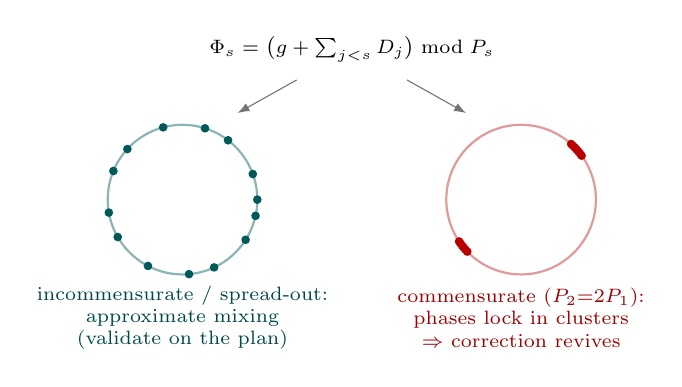
\begin{tikzpicture}[font=\footnotesize,x=1cm,y=1cm]
\colorlet{cmix}{teal!70!black}\colorlet{clock}{red!72!black}
% ---- left wheel: incommensurate -> equidistributed phases ----
\draw[thick,cmix!45] (0,0) circle (0.95);
\foreach \i in {0,...,13}{
  \fill[cmix] ({0.95*cos(137.5*\i)},{0.95*sin(137.5*\i)}) circle (0.055);}
\node[font=\scriptsize,align=center,cmix!80!black] at (0,-1.5)
  {incommensurate / spread-out:\\approximate mixing\\(validate on the plan)};
% ---- right wheel: commensurate -> locked phases ----
\begin{scope}[shift={(4.3,0)}]
\draw[thick,clock!40] (0,0) circle (0.95);
\foreach \a in {38,42,46,40,44,36,48}{
  \fill[clock] ({0.95*cos(\a)},{0.95*sin(\a)}) circle (0.055);}
\foreach \a in {216,220,224,218,222,214}{
  \fill[clock] ({0.95*cos(\a)},{0.95*sin(\a)}) circle (0.055);}
\node[font=\scriptsize,align=center,clock!85!black] at (0,-1.5)
  {commensurate ($P_2{=}2P_1$):\\phases lock in clusters\\$\Rightarrow$ correction revives};
\end{scope}
% phase annotation raised clear of both wheels; arrows start below it
\node[font=\scriptsize,align=center,anchor=south] at (2.15,1.62)
  {$\Phi_s=\bigl(g+\textstyle\sum_{j<s}D_j\bigr)\bmod P_s$};
\draw[-{Latex[length=1.5mm]},black!55] (1.45,1.52) -- (0.70,1.10);
\draw[-{Latex[length=1.5mm]},black!55] (2.85,1.52) -- (3.60,1.10);
\end{tikzpicture}
\caption{Phase mixing (random-offset property of
Section~\ref{sec:r2}, Remark~\ref{rem:fixedmix}). The arrival phase at
segment $s$ lives on a circle of circumference $P_s$. Under random
schedule offsets the wrapped phase is exactly uniform and independent
of the upstream increments; for a fixed plan with spread-out
(non-lattice) upstream delays and incommensurate periods the same
decoupling holds \emph{approximately} (left), and latencies compose by
convolution. Commensurate periods lock the phase into clusters (right):
the failure mode of a UAV synchronized to one specific LEO pass.}
\label{fig:mixing}
\end{figure}

Under paced generation with order-preserving deliveries
(Section~\ref{sec:model}; $Y_{\max}-Y_{\min}\le Z_{\min}$ suffices),
$\PAoIper=Z+Y$ and the single-copy mean needs no independence:
\begin{equation}
\E[\PAoIper{}^{(1)}]=\E[Z]+\sum_{s=1}^S(\E[R_s]+T_s),
\end{equation}
with deterministic envelope $\PAoIper{}^{(1)}\le Z_{\max}+\sum_s(G_s+T_s)$.

\begin{theorem}[$k{=}2$ per-update PAoI, phase-mixing regime]\label{thm:r2}
With i.i.d.\ copy latencies $Y^{(1)},Y^{(2)}\sim F_Y$, where $F_Y$ is
the common cumulative distribution function of the single-copy latency
$Y$, and $\Ymin=\min(Y^{(1)},Y^{(2)})$,
\begin{align}
\E[\PAoIper{}^{(2)}]&=\E[Z]+\int_0^\infty[1-F_Y(y)]^2\,dy,\\
\E[\Ymin]&=\E[Y]-\tfrac12\,\E\bigl|Y^{(1)}-Y^{(2)}\bigr|\le\E[Y],
\end{align}
with equality iff $Y$ is deterministic.
\end{theorem}

\begin{remark}[Cadence, dispersion, and what replication buys]
Replication leaves the \emph{generation} cadence unchanged (one reset
per \emph{delivered} update, at its earliest surviving copy; an update
losing all copies produces none), so in the lossless limit
the mean inter-delivery interval is invariant, $\E[Z']{=}\E[Z]$, and
replication acts only through $\Ymin$, whose saving is exactly half
the mean absolute difference of path latencies (the standard
Gini-mean-difference identity): largest at sparse, high-dispersion
contacts and nearly nil on near-deterministic links. The invariance is a
mean-rate statement only: with losses or reordering, replication also
\emph{tightens the distribution} of $Z$ (fewer long fault-induced
outage gaps); Proposition~\ref{prop:uncertain} quantifies this cadence
effect. Shrinking the mean cadence itself requires $k$ independent
update streams, a different energy trade (the fresh-sample-per-route
case of Section~\ref{sec:model}).
\end{remark}

\begin{remark}[Worked ratio and general $k$]
For two ensemble-phase satellites with $Y\approx R+T_s$,
$\E[\Rmin]/\E[R]=\tfrac23(1-\delta)$, a ${\approx}33\%$ cut of the
gating term at sparse contacts (Fig.~\ref{fig:r2gain}).
$\E[Y_{\min,k}]=\int_0^\infty(1-F_Y)^k$ generalizes, but closed forms
past $k{=}2$ with multi-segment convolutions are unwieldy; we use a
recursive numerical evaluation for general $k$. The minimum identity
assumes copies traverse \emph{independent} contacts; same-bottleneck
copies give $Y^{(1)}{=}Y^{(2)}$ and zero gain.
\end{remark}

% AUTO-GENERATED by figs/make_figures.py -- do not edit.
\begin{figure}[t]\centering
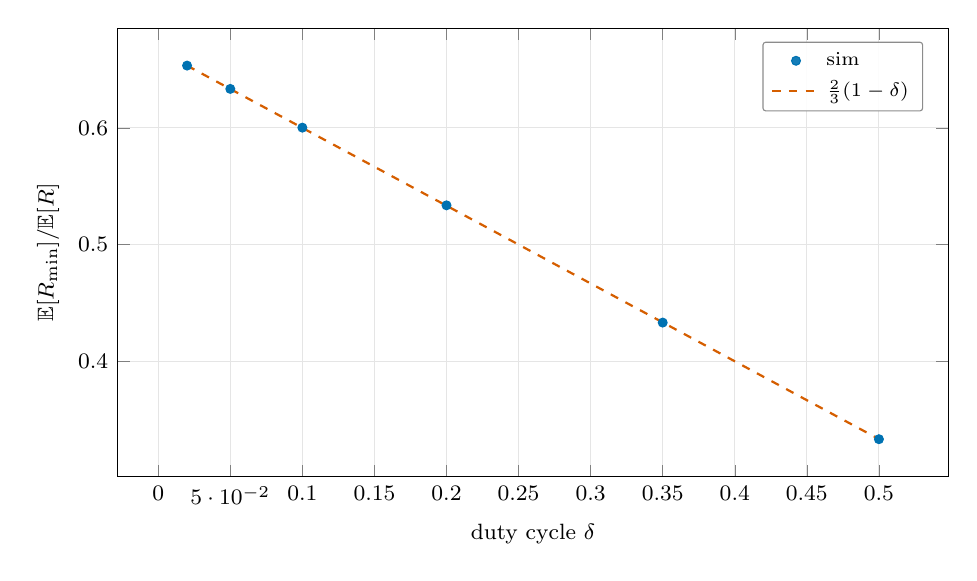
\begin{tikzpicture}
\begin{axis}[paperfig,width=\columnwidth,height=0.6\columnwidth,
  xlabel={duty cycle $\delta$},ylabel={$\mathbb{E}[R_{\min}]/\mathbb{E}[R]$},
  legend pos=north east,grid=both,legend cell align=left]
\addplot[cA,only marks,mark=*,mark size=1.6pt] coordinates {(0.02,0.653362323347421) (0.05,0.6333883269504517) (0.1,0.6001979804547108) (0.2,0.5336253055696409) (0.35,0.433159970801058) (0.5,0.33323957490210027)};
\addlegendentry{sim}
\addplot[cB,no marks,thick,dashed] coordinates {(0.02,0.6533333333333333) (0.05,0.6333333333333333) (0.1,0.6) (0.2,0.5333333333333333) (0.35,0.43333333333333335) (0.5,0.3333333333333333)};
\addlegendentry{$\tfrac{2}{3}(1-\delta)$}
\end{axis}
\end{tikzpicture}
\caption{Result~2 (E4): the two-copy gain. Simulated
$\mathbb{E}[R_{\min}]/\mathbb{E}[R]$ matches the two-copy
ratio $\tfrac{2}{3}(1-\delta)$; replication saves most at sparse
contacts ($\delta\to0$).}
\label{fig:r2gain}
\end{figure}


% =====================================================================
\section{Result 3: Energy--Replication Threshold}\label{sec:r3}
Replicating a bundle over several contacts lowers its delivered latency
(the freshest copy wins) but each copy drains the relay's battery, so
there is a best number of copies to send; this section finds it. Deterministic, common service $T_s$ is an additive constant in
the peak, so the only $k$-dependent term is the LEO gating term. The
delivered residual over $k$ contacts is, in full generality, an integral
of the \emph{joint} survival,
\begin{equation}\label{eq:rminjoint}
\E[R_{\min,k}]=\int_0^\infty\Pr\bigl(R_1>r,\dots,R_k>r\bigr)\,dr,
\end{equation}
and how it evaluates depends on the plan model, because the $k$
residuals are functions of a \emph{common} arrival instant and are not
automatically independent, even for staggered windows:
\begin{enumerate}
\item[(i)] \emph{Random-offset ensemble.} If each
copy's schedule offset $\Theta_i$ is an independent uniform on
$[0,P)$, the wrapped phases $U-\Theta_i$
are i.i.d.\ uniform, the $R_i$ are \emph{exactly} i.i.d.\ with the
residual
law of Section~\ref{sec:r1}, and \eqref{eq:rminjoint} factorizes:
\begin{align}
\E[R_{\min,k}]&=\int_0^\infty\prod_{i=1}^{k}\Pr(R_i>r)\,dr
\label{eq:rminprod}\\
&=\int_0^{G}\!\Bigl(\frac{G-r}{P}\Bigr)^k dr
=\frac{P(1-\delta)^{k+1}}{k+1},\label{eq:rmink}
\end{align}
with $G=P(1-\delta)$. (Consistency: $k{=}1$ recovers
Theorem~\ref{thm:r1}; heterogeneous marginals use
\eqref{eq:rminprod} directly.) For a \emph{fixed} plan whose copy
routes have pairwise incommensurate periods, the relative phases drift,
and the same product form is a \emph{time-average approximation} over
the horizon, not exact independence, since all residuals share the
arrival instant (Remark~\ref{rem:fixedmix}); its accuracy is checked on
the plan, and otherwise the exact joint form \eqref{eq:rminjoint}
applies.
\item[(ii)] \emph{Fixed co-period plan.} With deterministic offsets the
joint survival must be evaluated on the plan; it is deterministic and
\emph{computable at planning time}. For $k$ windows evenly staggered by
$P/k$ the union schedule is a single comb of period $P/k$, so (with
$x_+=\max\{x,0\}$)
\begin{equation}\label{eq:rminstag}
\E[R_{\min,k}]=\frac{P}{2k}\,(1-k\delta)_+^2,
\end{equation}
(derivation: the comb has gap $P/k-W$ per period $P/k$, so the residual
law of Section~\ref{sec:r1} applies with $(P,W)\to(P/k,W)$ and
$\E[R]=(P/k-W)^2/(2P/k)$), \emph{better} than the ensemble value
\eqref{eq:rmink}: deterministic
anti-phasing beats blind placement. Once $k\delta\ge1$ the staggered
comb covers the entire period: the residual is zero, the gain profile
is flat, and further copies cannot improve the gating term, so the
smallest covering degree $\lceil1/\delta\rceil$ is the
energy-conserving choice. The threshold analysis below operates on the
strictly decreasing range $k\delta<1$.
\item[(iii)] \emph{Locked phases.} Coincident offsets give
$\E[R_{\min,k}]=\E[R]$: zero gain.
\end{enumerate}
The extremal fixed plans and the ensemble form a reference ladder, the
\emph{phase ladder}
\begin{equation}\label{eq:ladder}
\underbrace{\frac{P}{2k}(1-k\delta)_+^2}_{\text{even stagger}}
\;\le\;
\underbrace{\frac{P(1-\delta)^{k+1}}{k+1}}_{\text{phase-agnostic}}
\;\le\;
\underbrace{\frac{P}{2}(1-\delta)^2}_{\text{locked}},
\end{equation}
with equality throughout at $k{=}1$. The outer terms are the extremal
fixed plans (best and worst deterministic offsets); the middle term is
the \emph{ensemble} reference, not a separator, since an individual
fixed plan can land anywhere in the outer interval, on either side of it. This
is exactly the ordering
measured on real Iridium-NEXT pairs in Section~\ref{sec:sim}
(residual-min ratio $0.41$ anti-phased, $0.61$ ensemble reference,
$0.95$ near-locked, with intermediate pairs scattered on both sides). We develop the threshold below for the
\emph{phase-agnostic} profile (i), the operative model when copy
routes have drifting relative phases or are assigned without phase
information, and note that every structural result carries over to
profile (ii) with \eqref{eq:rminstag} in place of \eqref{eq:rmink} on
its strictly decreasing range $k\delta<1$ (beyond full coverage the
profile is flat and the smallest covering degree is optimal).

\paragraph*{Energy-adequacy ratio}
Measuring energy in copies (harvest $\lambda_e/e$ copies per unit
time, contact rate $\lambda_c=1/P$), define
\begin{equation}
\eta\triangleq\frac{\lambda_e/e}{\lambda_c}=\frac{\lambda_e P}{e}
\quad\text{(copies harvested per period).}
\end{equation}
Demanding $k$ copies per period caps the launchable fraction of update
epochs at $\peff(k)=\min(1,\eta/k)$ (flow balance; derived exactly in
Section~\ref{sec:r3hard}). Two modeling choices are made explicit here,
because the objective inherits them. \emph{Fixed cadence:} the source
samples once per period at an epoch exogenous to the plan
(Section~\ref{sec:model}); the budget is spent on copies, not on a
higher sampling rate. \emph{All-or-nothing firing:} at a firing epoch
the source launches all $k$ copies if the battery holds $k$ units and
otherwise launches none, holding its energy for the next epoch. This is
the atomic-admission semantics of a bundle with $k$ pre-committed
routes (the copies are enqueued together, as our CGR-native router
does), and it keeps every fired update's peak of one form, so that the
mean objective below is exact given the firing fraction. It is a
restriction, not an optimum: Section~\ref{sec:sim} measures its price
against rules that fire a partial degree ($1.4$--$2.7\%$, in the
transition and energy-abundant regimes of the configuration tested).
Under these two choices every epoch that fires delivers one update
whose peak is $JP+R_{\min,k}+T_s$, where $J\ge1$ is the number of
periods since the previous firing. The residual is independent of the
battery, and $\E[J]=1/\peff$ for any stationary, ergodic firing
sequence (Palm inversion: the mean spacing between firings is the
reciprocal of their long-run fraction), so
$\E[\PAoIper]=P/\peff+\E[R_{\min,k}]+T_s$; under i.i.d.\ firing $J$ is
in addition geometric. Dropping the
$k$-independent constant $P+T_s$ gives the
mean-$\PAoIper$ gating objective
\begin{equation}\label{eq:obj}
\mathcal{A}(k)=
\underbrace{P\,\frac{1-\peff(k)}{\peff(k)}}_{\text{starvation}}
+\underbrace{\frac{P(1-\delta)^{k+1}}{k+1}}_{\text{gain}},
\quad\peff(k)=\min\Bigl(1,\frac{\eta}{k}\Bigr).
\end{equation}
(The gain term enters unweighted by $\peff$: a fired update's copies
realize $R_{\min,k}$ whether or not earlier epochs were skipped, and
the skips are already counted in $J$. For example, at $\eta{=}1$,
$k{=}2$, $\delta{=}0.1$ the simulated mean peak is $2.246P$ against
$2.248P$ from this accounting, whereas weighting the gain by $\peff$
would give $2.127P$.)
For $k\le\eta$ the starvation term vanishes and $\mathcal{A}$ is strictly
decreasing; for $k>\eta$ the starvation term equals
$\frac{P}{\eta}(k-\eta)$ and rises linearly while the gain term decays.
Hence $\mathcal{A}$ is unimodal and its minimizer is one of the two
integers bracketing $\eta$:
\begin{equation}\label{eq:kstar}
\kstar=\min\bigl(K_{\max},\,k^{\circ}\bigr),\quad
k^{\circ}\in\{\lfloor\eta\rfloor,\lceil\eta\rceil\},\quad
\eta=\frac{\lambda_e P}{e}.
\end{equation}
Here $\lfloor\eta\rfloor$ is the largest degree that incurs \emph{no}
starvation, the conservative DTN-reliability rule, while the skip-aware
optimum takes the extra copy, $k^{\circ}{=}\lceil\eta\rceil$, iff its
added starvation is repaid by the order-statistic gain:
\begin{equation}\label{eq:ceiltest}
P\Bigl(\frac{\lceil\eta\rceil}{\eta}-1\Bigr)<g_{\lfloor\eta\rfloor}-g_{\lceil\eta\rceil},
\qquad g_k=\frac{P(1-\delta)^{k+1}}{k+1}.
\end{equation}
(For integer $\eta$, $\kstar{=}\eta$; $\kstar{=}1$ if $\eta<1$.)
$K_{\max}$ is the number of available copy routes. The
distinction between the conservative rule $\lfloor\eta\rfloor$ and the
skip-aware optimizer is itself a contribution, because occasional energy-forced
skips can be worth an extra copy near the top of an integer interval.
Fig.~\ref{fig:r3unimodal} shows the simulated mean $\PAoIper$ as a
function of $k$ at $\eta{=}3$ and $\eta{=}5$: unimodal, with the minimum
at $k{=}\eta$ (E7).

\begin{remark}[Conditionality and gain-profile generality]
\label{rem:gainprofile}
Everything above is conditional on (a) \emph{all-or-nothing} firing and
(b) the \emph{phase-agnostic} gain profile
$g_k=P(1-\delta)^{k+1}/(k+1)$ of plan model (i). The structure
generalizes with one quantitative caveat. For any strictly decreasing
gain profile with diminishing increments ($g_k-g_{k+1}\ge
g_{k+1}-g_{k+2}$ for all $k$), $\mathcal{A}$ is unimodal
(the starvation term is zero up to $\eta$ and rises linearly beyond
it), and Theorem~\ref{thm:r3}'s monotonicity holds. The
\emph{two-candidate bracketing} $k^\circ\in\{\lfloor\eta\rfloor,
\lceil\eta\rceil\}$ additionally requires that the first forward gain
drop beyond the threshold not exceed the starvation slope,
\begin{equation}\label{eq:gainbound}
g_{\lceil\eta\rceil}-g_{\lceil\eta\rceil+1}\;\le\;\frac{P}{\eta};
\end{equation}
diminishing increments then keep the forward difference
$\Delta_k\mathcal{A}\triangleq\mathcal{A}(k{+}1)-\mathcal{A}(k)\ge0$ for all
$k\ge\lceil\eta\rceil$. Without \eqref{eq:gainbound} the rule can fail
(e.g.\ $g_k\propto c/k$ with large $c$ places the optimum far above
$\lceil\eta\rceil$ while satisfying diminishing increments). Both plan
models satisfy \eqref{eq:gainbound} automatically: for (i), $g_k\le
P/(k+1)$, and for the even-stagger profile
$g^{\mathrm{stag}}_k=\tfrac{P}{2k}(1-k\delta)_+^2$ of plan model (ii),
$g^{\mathrm{stag}}_k\le P/(2k)$; in
both cases the drop at $k=\lceil\eta\rceil$ is below
$P/\lceil\eta\rceil\le P/\eta$ since
$\eta\le\lceil\eta\rceil$. The same floor/ceiling policy therefore
applies to a deterministically staggered plan with $g^{\mathrm{stag}}$
replacing $g$ in \eqref{eq:ceiltest}---only the crossover points move.
For a general fixed plan, $g_k$ is computed from \eqref{eq:rminjoint}
at planning time and \eqref{eq:gainbound} is checked alongside.
\end{remark}

\begin{theorem}[Monotonicity and saturation]\label{thm:r3}
For any strictly decreasing gain profile $g_k$ with diminishing
increments, $\kstar(\eta)$ is non-decreasing in
$\eta=\lambda_e/(\lambda_c e)$, and is
constant at $K_{\max}$ for all $\eta\ge K_{\max}$.
\end{theorem}
\begin{proof}
Write $\mathcal{A}=g+H$ with
$H(k;\eta)=P\max(0,k/\eta-1)$. The forward difference $\Delta_k g<0$ is
independent of $\eta$, while
$\Delta_k H(k;\eta)=\tfrac{P}{\eta}\min\bigl(1,(k{+}1-\eta)_+\bigr)\ge0$
(equal to $P/\eta$ for $k\ge\eta$, to $0$ for $k{+}1\le\eta$, linear
between) is non-increasing in $\eta$ for each fixed $k$. Hence
$\Delta_k\mathcal{A}$ is non-increasing in $\eta$, so the first
up-crossing $\kstar(\eta)=\min\bigl(\{k:\Delta_k\mathcal{A}\ge0\}
\cup\{K_{\max}\}\bigr)$ is
non-decreasing in $\eta$. For $\eta\ge K_{\max}$, $\Delta_k H=0$ over the
feasible range, so $\mathcal{A}=g$ is strictly decreasing and the
minimizer is pinned at $K_{\max}$.
\end{proof}
Fig.~\ref{fig:r3kstar} shows the simulated optimal degree as a function
of $\eta$ (E8): a non-decreasing staircase that saturates at
$K_{\max}{=}8$.

% AUTO-GENERATED by figs/make_figures.py -- do not edit.
\begin{figure}[t]\centering
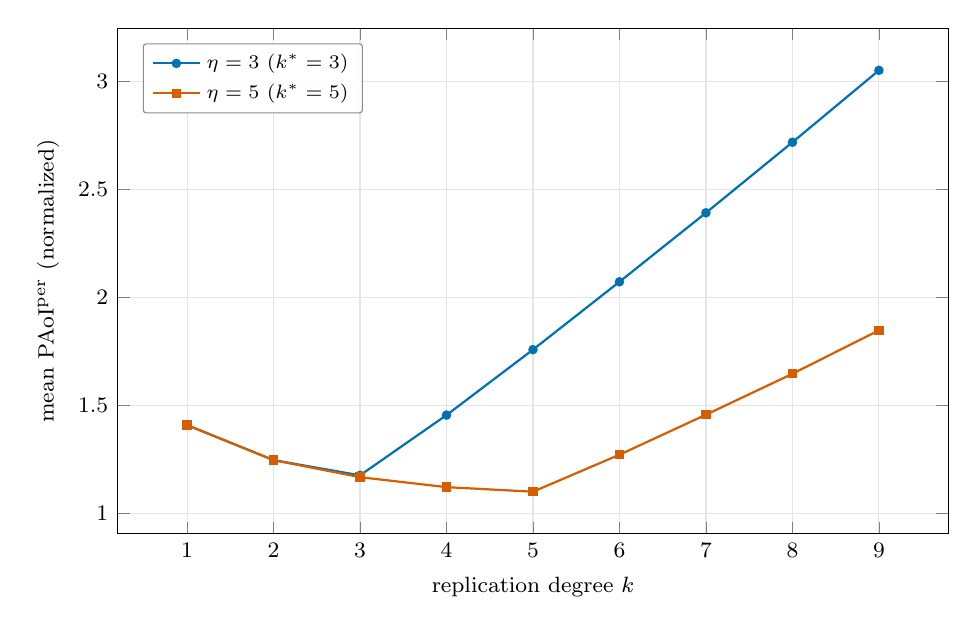
\begin{tikzpicture}
\begin{axis}[paperfig,width=\columnwidth,height=0.66\columnwidth,
  xlabel={replication degree $k$},ylabel={mean $\PAoIper$ (normalized)},
  legend pos=north west,grid=both,legend cell align=left,xtick=data]
\addplot[thick,cA,mark=*,mark size=1.3pt] coordinates {(1.0,1.410314663389778) (2.0,1.248192570863487) (3.0,1.1777586195908003) (4.0,1.4564704134531814) (5.0,1.7592147238268279) (6.0,2.073176697683509) (7.0,2.3922001335971532) (8.0,2.7185592470423137) (9.0,3.0510884750494167)};
\addlegendentry{$\eta=3$ ($k^\ast=3$)}
\addplot[thick,cB,mark=square*,mark size=1.3pt] coordinates {(1.0,1.4101859347850572) (2.0,1.2478719880669222) (3.0,1.1692371885105677) (4.0,1.123112635056019) (5.0,1.1020916179657483) (6.0,1.2732102430111434) (7.0,1.458191515479616) (8.0,1.6476294592829408) (9.0,1.8487261126269243)};
\addlegendentry{$\eta=5$ ($k^\ast=5$)}
\end{axis}
\end{tikzpicture}
\caption{Result~3 (E7): the integrated energy+replication+AoI objective
is unimodal in $k$ with minimum at one of the two integers bracketing
$\eta$; pushing
$k$ past the energy budget starves future contacts and raises the peak.}
\label{fig:r3unimodal}
\end{figure}

% AUTO-GENERATED by figs/make_figures.py -- do not edit.
\begin{figure}[t]\centering
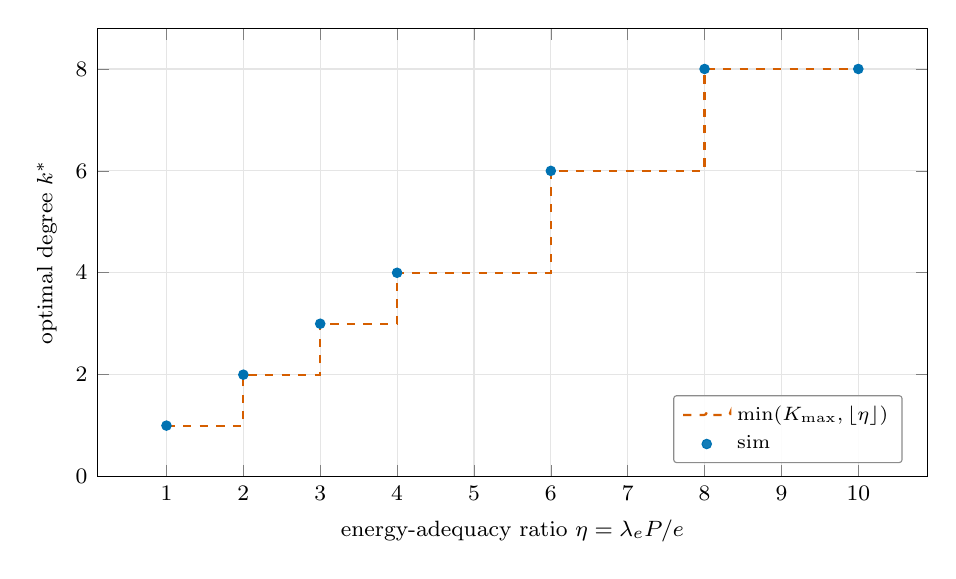
\begin{tikzpicture}
\begin{axis}[paperfig,width=\columnwidth,height=0.6\columnwidth,
  xlabel={energy-adequacy ratio $\eta=\lambda_e P/e$},ylabel={optimal degree $k^\ast$},
  legend pos=south east,grid=both,legend cell align=left,ymin=0]
\addplot[cB,no marks,thick,dashed,const plot] coordinates {(1.0,1.0) (2.0,2.0) (3.0,3.0) (4.0,4.0) (6.0,6.0) (8.0,8.0) (10.0,8.0)};
\addlegendentry{$\min(K_{\max},\lfloor\eta\rfloor)$}
\addplot[cA,only marks,mark=*,mark size=1.7pt] coordinates {(1.0,1.0) (2.0,2.0) (3.0,3.0) (4.0,4.0) (6.0,6.0) (8.0,8.0) (10.0,8.0)};
\addlegendentry{sim}
\end{axis}
\end{tikzpicture}
\caption{Result~3 (E8): $k^\ast(\eta)$ is non-decreasing in the
harvest-to-contact ratio and saturates at $K_{\max}{=}8$ once energy
ceases to bind.}
\label{fig:r3kstar}
\end{figure}


\begin{remark}[Interpretation]
$\kstar$ tracks the harvest-to-contact ratio: launch as many independent
copies as the energy budget sustains without forcing skipped windows, and
no more. Over-replication ($k>\eta$) drains the battery and starves
future contacts, so the linear starvation term overwhelms the vanishing
order-statistic gain. When harvest covers full contact diversity
($\eta\ge K_{\max}$) energy stops binding and $\kstar=K_{\max}$; when
$\eta<1$, $\kstar=1$ (no replication), matching the energy-harvesting AoI
result that aggressive replication is sub-optimal once harvest rate falls
below the update rate.
\end{remark}

\begin{remark}[Where the replication gain comes from]
\label{rem:uncertainty}
Deterministic scheduling by itself produces \emph{no} strict replication
benefit: under a fault-free, exactly known contact plan, an oracle
single-copy router (CGR with the true plan) already selects the
earliest-arriving route, so $\min_i Y^{(i)}$ is attained with one copy
and higher degrees can only \emph{tie}, as our Tier-2 experiment
confirms on a fault-free staggered diamond (Section~\ref{sec:sim}). The
strict gain characterized in this section is operative precisely under
\emph{route-outcome uncertainty}, of which our framework instantiates
three forms: (a) \emph{plan uncertainty}, in which the phase-agnostic
(random-offset) model treats the copy phases as unknown at decision
time, so no single route is knowably earliest; (b) \emph{outcome
uncertainty}, in which relay faults break the nominally earliest
route (quantified model-exactly in Section~\ref{sec:sim}); and (c)
\emph{prediction error} in the contact plan itself
(Section~\ref{sec:policy}). The deterministic residual and renewal laws
are thus the \emph{structure} against which the gain is computed, since
they set the gain profile $g_k$, while uncertainty is the \emph{source}
of the gain. This is
also why predictable space-DTN routing conventionally avoids
duplication: with no uncertainty, it buys nothing.
\end{remark}

\paragraph*{Uncertainty-aware threshold}
Remark~\ref{rem:uncertainty} identifies uncertainty as the source of the
gain; we now fold it into the optimization itself, since \eqref{eq:obj}
is a \emph{lossless} analysis in which every fired update eventually
resets the age. Let each
copy \emph{succeed} with probability $q$ (its route materializes and
delivers), with energy spent on the launch regardless; successes are
i.i.d.\ across copies and periods and independent of the copies'
contact phases and residuals.
An admitted update then succeeds with probability
$s_k=1-(1-q)^k$, and the delivered residual is the minimum over the
$\mathrm{Bin}(k,q)$ surviving copies. Let $h_k(q)$ denote the
conditional mean of that minimum given at least one survivor. Since a
copy enters the minimum only if it survives,
$\Pr(\text{every survivor exceeds }r)=\bigl(1-q+q\Pr(R>r)\bigr)^k$, and
subtracting the no-survivor event and integrating the survival over
the gap gives, for the phase-agnostic profile,
\begin{equation}\label{eq:hq}
\begin{aligned}
h_k(q)&=\frac{1}{s_k}\int_0^{G}\Bigl[\Bigl(1-q+q\,\frac{G-r}{P}\Bigr)^{k}
-(1-q)^{k}\Bigr]dr\\
&=\frac{1}{s_k}\Bigl[\frac{P\bigl[(1-q\delta)^{k+1}-(1-q)^{k+1}\bigr]}{q(k+1)}
-G(1-q)^{k}\Bigr],
\end{aligned}
\end{equation}
with $h_k(1)=g_k$ and $h_1(q)=\E[R]$.

\begin{proposition}[Peak age under route uncertainty]\label{prop:uncertain}
Under paced generation, all-or-nothing firing, order-preserving
successful deliveries (Section~\ref{sec:model}), and the i.i.d.\
success model above:
(i)~in stationarity the successful-update rate is $\peff s_k$ per
period, so
\begin{equation}\label{eq:objq}
\begin{aligned}
\E[\PAoIper]&=\frac{P}{\peff(k)\,s_k}+h_k(q)+T_s,\\
\mathcal{A}_q(k)&=P\,\frac{1-\peff s_k}{\peff s_k}+h_k(q),
\end{aligned}
\end{equation}
by the stationary successful-update rate (the inter-success spacing is
geometric only in the
i.i.d.-admission special case; the \emph{mean} needs only the rate);
(ii)~$\mathcal{A}_q$ is strictly decreasing on $k\le\lfloor\eta\rfloor$
(there $\peff=1$, $s_k$ is strictly increasing, and $h_k$ is strictly
decreasing, because the number of surviving copies given at least one
survivor is stochastically increasing in $k$ and $g_n$ is strictly
decreasing in $n$); and
(iii)~for $k\ge\eta$ the cadence increment is nonnegative,
\begin{equation}\label{eq:dphi}
\Delta_k\Bigl(\frac{k}{s_k}\Bigr)
=\frac{s_k-kq(1-q)^k}{s_k\,s_{k+1}}\;\ge\;0,
\end{equation}
since $s_k=q\sum_{j<k}(1-q)^j\ge kq(1-q)^{k-1}\ge kq(1-q)^k$; hence the
minimizer lies in $\{\lfloor\eta\rfloor,\lceil\eta\rceil\}$ whenever the
increment condition
\begin{equation}\label{eq:gainboundq}
\frac{P}{\eta}\,\Delta_k\Bigl(\frac{k}{s_k}\Bigr)\;\ge\;
h_k(q)-h_{k+1}(q)\qquad\forall\,k\ge\lceil\eta\rceil
\end{equation}
holds, the uncertainty analog of \eqref{eq:gainbound}. At $q=1$,
\eqref{eq:gainboundq} reduces to \eqref{eq:gainbound} and the
proposition recovers \eqref{eq:obj}--\eqref{eq:kstar} exactly.
\end{proposition}

Throughout, the candidate set is clipped to $[1,K_{\max}]$ as in
\eqref{eq:policy}: for $\eta<1$ the floor is infeasible and $k{=}1$ is
the lower candidate.
Parts (i)--(iii) are proved; what is \emph{not} claimed as a theorem is
that \eqref{eq:gainboundq} holds universally. Since
\eqref{eq:gainboundq} depends on $\delta$ through $h_k(q)$, we verified
it, together with the resulting clipped two-candidate optimum, over the full
grid $\delta\in[0.02,0.9]\times q\in[0.05,1]\times\eta\in[0.1,8]$
($840$ points, $k\le12$): the condition holds with minimum margin
$0.067P$ (attained at small $\delta$, small $q$, large $\eta$) and the
optimizer never left the candidate set
(\texttt{check\_gainboundq.py} in the artifact); E18
(Section~\ref{sec:sim}) confirms the same in simulation. For
parameters outside these ranges
\eqref{eq:gainboundq} is a one-line numerical check performed alongside
the policy, exactly as \eqref{eq:gainbound} is for fixed plans.

The structural change at $q<1$ is that replication now buys
\emph{cadence} as well as latency spread: the failure-gap term
$P(1-s_k)/s_k$ decays geometrically in $k$. Here $q$ is the
\emph{effective per-pass route-success probability}, which is not the
relay's duty-cycle availability. In the unified Tier-2 experiment
(Section~\ref{sec:sim}) a relay that is down one third of the time
still delivers every update with bounded delay inflation, because a
copy that misses its pass can be re-routed and arrive later; this is
consistent with an effective $q$ close to one, although eventual
delivery alone does not determine the per-pass value. How far below the
availability $q$ falls depends on how often a stall becomes a missed
pass, that is, on the alternatives the plan offers. We propose to
estimate $\hat q$ directly, as the fraction of admitted single-copy
updates that succeed on their operative pass, and to cross-check it
against the observed inter-success cadence through
$\E[Z_{\mathrm{succ}}]=P/(\peff\,\hat q)$; the estimator is not
evaluated in this paper.

The i.i.d.\ Bernoulli model is a first-order approximation: it omits
fault-dwell correlation, that is, failures that cluster across
consecutive passes (tested in experiment E19, Section~\ref{sec:sim}).
The contact-prediction experiment of Section~\ref{sec:policy}, in
contrast, is an exact instance of the i.i.d.\ $q$-model, because its
prediction reliability is $q$ by construction. Evaluating
\eqref{eq:objq} at its parameters reproduces the observed ordering:
keeping $k{=}\lfloor\eta\rfloor$ beats the reserve heuristic
$\lfloor q\eta\rfloor$ (at $\eta{=}6$ and $q{=}0.4$,
$\mathcal{A}_{0.4}(6)=0.28P$ versus $\mathcal{A}_{0.4}(2)=0.93P$). That
empirical finding is therefore a prediction of the theory.

% =====================================================================
\section{Hardening: Work-Conserving Battery-Queue Throttle}\label{sec:r3hard}
The throttle $\peff=\min(1,\eta/k)$ used above was a fluid approximation.
In reality the relay's battery is a finite queue that fills as energy is
harvested and drains $k$ units each time it fires $k$ copies
(Fig.~\ref{fig:battpath}); we now
replace the fluid throttle by the stationary law of this energy queue and
couple it to the age dynamics.

\paragraph*{Energy queue}
Let the battery hold up to $B$ units (one unit $=$ the energy $e$ to send
one copy) and harvest $A$ units per contact period, i.i.d.\ across periods
with mean $\E[A]=\eta$ (the harvest-per-period in copies; Poisson for the
explicit chain). Under the all-or-nothing policy (fire $k$ copies iff
$b\ge k$, else hold and recharge) the embedded chain at
contact epochs is
\begin{equation}
b_{n+1}=\min\!\Bigl(B,\ \bigl(b_n-k\,\ind\{b_n\ge k\}\bigr)+A_n\Bigr),
\end{equation}
a finite chain on $\{0,\dots,B\}$. For Poisson harvest (support all of
$\mathbb{N}_0$) the chain is irreducible and aperiodic on
$\{0,\dots,B\}$ with a unique stationary $\pi$; the throttle is
$\peff(k)=\Prob_\pi(b\ge k)$. No simple positivity condition
substitutes for this support assumption: $\Pr(A{\ge}1)>0$ alone fails
($A\in\{0,2\}$ with $k{=}2$ traps a parity class), and even
$\Pr(A{=}0)>0$ with $\Pr(A{=}1)>0$ fails (Bernoulli $A\in\{0,1\}$ with
$k{=}2$ never accumulates past $b{=}k$, leaving the states above $k$
unreachable). In general we assume the harvest support induces an
irreducible, aperiodic transition graph on the reachable battery
states. Otherwise, including lattice or deterministic harvest (e.g.\
$A\equiv\eta\in\mathbb{N}$ cycles deterministically), $\pi$ and
$\peff$ are read on the recurrent class reachable from $b_0$, which
exists by finiteness, and the work-conservation
identity below holds under \emph{any} stationary regime, since it is a
flow balance that never invokes ergodic structure.

\begin{figure}[t]
\centering
\resizebox{\columnwidth}{!}{%
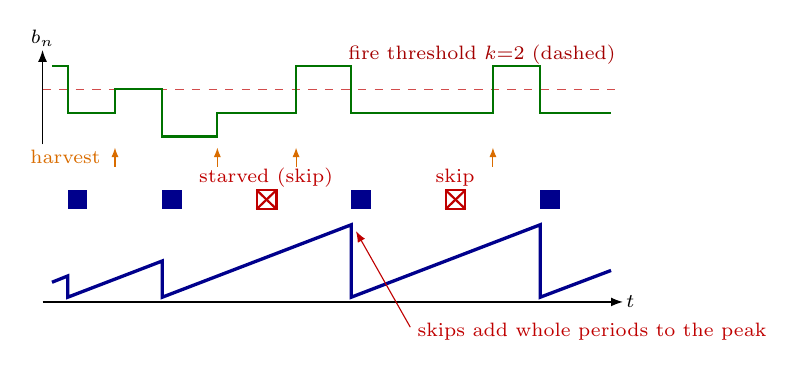
\begin{tikzpicture}[font=\footnotesize,x=1cm,y=1cm]
\colorlet{cbat}{green!45!black}\colorlet{cfire}{blue!55!black}
\colorlet{cskip}{red!75!black}\colorlet{cage}{blue!55!black}
\colorlet{charv}{orange!85!black}
% ===== battery staircase (top band), k=2; levels: b -> 2.1+0.3b =====
\draw[-{Latex[length=1.5mm]}] (-0.12,2.0)--(-0.12,3.2) node[above,font=\scriptsize,inner sep=1pt]{$b_n$};
\draw[dashed,cskip!70] (-0.12,2.7)--(7.25,2.7);
\node[font=\scriptsize,cskip!85!black,anchor=east,inner sep=1pt] at (7.2,3.14) {fire threshold $k{=}2$ (dashed)};
\draw[thick,cbat]
 (0,3.0)--(0.2,3.0)--(0.2,2.4)--(0.8,2.4)--(0.8,2.7)--(1.4,2.7)
 --(1.4,2.1)--(2.1,2.1)--(2.1,2.4)--(3.1,2.4)--(3.1,3.0)--(3.8,3.0)
 --(3.8,2.4)--(5.6,2.4)--(5.6,3.0)--(6.2,3.0)--(6.2,2.4)--(7.1,2.4);
% harvest arrows (below battery band)
\foreach \x in {0.8,2.1,3.1,5.6}{
  \draw[-{Latex[length=1.2mm]},charv] (\x,1.72)--(\x,1.96);}
\node[font=\scriptsize,charv,anchor=east,inner sep=1pt] at (0.66,1.84) {harvest};
% ===== contact comb (middle band): fired (filled) vs starved (crossed) =====
\foreach \x in {0.2,1.4,3.8,6.2}{
  \fill[cfire] (\x,1.18) rectangle (\x+0.25,1.42);}
\foreach \x in {2.6,5.0}{
  \draw[thick,cskip] (\x,1.18) rectangle (\x+0.25,1.42);
  \draw[thick,cskip] (\x,1.18)--(\x+0.25,1.42);
  \draw[thick,cskip] (\x,1.42)--(\x+0.25,1.18);}
\node[font=\scriptsize,align=center,inner sep=1pt,cskip] at (2.72,1.58) {starved (skip)};
\node[font=\scriptsize,align=center,inner sep=1pt,cskip] at (5.12,1.58) {skip};
% ===== age sawtooth (bottom band): resets only at fired windows =====
\draw[-{Latex[length=1.5mm]}] (-0.12,0)--(7.25,0) node[right,font=\scriptsize,inner sep=1pt]{$t$};
\draw[very thick,cage]
 (0,0.25)--(0.2,0.33)--(0.2,0.06)--(1.4,0.52)--(1.4,0.06)
 --(3.8,0.98)--(3.8,0.06)--(6.2,0.98)--(6.2,0.06)--(7.1,0.4);
\draw[-{Latex[length=1.4mm]},cskip] (4.55,-0.32) -- (3.86,0.9);
\node[font=\scriptsize,cskip,anchor=west,inner sep=1pt] at (4.6,-0.38)
  {skips add whole periods to the peak};
\end{tikzpicture}}
\caption{Energy-gated firing, sample path ($k{=}2$). \emph{Top:} the
battery fills by harvest and drops $k$ units at each firing; a window
that opens with $b<k$ is \emph{starved} and skipped (crossed).
\emph{Bottom:} the age resets only at fired windows, so each skip adds a
full period to the peak $JP+R_{\min}+T_s$, which is the starvation term
$P(1-\peff)/\peff$ of \eqref{eq:obj}. After a firing the battery is
depleted, which is why consecutive windows are correlated
(Markov-renewal gaps) and the fluid throttle is a mean-field limit.}
\label{fig:battpath}
\end{figure}

\begin{lemma}[Work conservation; distribution-free]\label{lem:work}
Each firing slot consumes exactly $k$ units, so in steady state
$k\,\peff(k)=\eta-L$ with $L\ge0$ the mean per-period harvest lost to the
cap. Hence
\begin{equation}
\peff(k)=\frac{\eta-L}{k}\le\min\!\Bigl(1,\frac{\eta}{k}\Bigr),
\end{equation}
with $L=0$ iff no harvested energy is truncated by the cap (the battery
may reach $B$ exactly without loss; only overflowed harvest counts).
\end{lemma}

Only the mean $\eta$ enters at this order; the harvest distribution and
$B$ affect $\peff$ solely through $L$. Thus the throttle of
Section~\ref{sec:r3} is exactly the no-overflow / large-$B$ limit, and
the finite-battery correction is sign-definite ($\peff$ can only be
smaller).

\begin{corollary}[$k=1$ closed form]
Let the per-period harvest increments $A_n$ be i.i.d., nonnegative,
with $\E[A_n]=\eta$ and $\Prob(A_n{=}0)>0$, so the chain
$b_{n+1}=(b_n-1)_+ + A_n$, the
embedded queue-length chain of a discrete-time deterministic-unit-service
queue, is ergodic on the recurrent class reachable from $b_0$ for
$\eta<1$ (all of $\mathbb{N}_0$ under unbounded support, e.g.\
Poisson; trivially for finite $B$); the stated marginals below follow
from flow balance and are class-independent. For $B\to\infty$ and
$\eta<1$, $\Prob_\pi(b=0)=1-\eta$, so $\peff(1)=\eta$, with the
Pollaczek--Khinchine level law. Finite $B$ gives $L\ge0$ and
$\peff(1)\le\eta$, with \emph{strict} loss exactly when overflow has
positive stationary probability, as under Poisson harvest for any
finite $B$, but not universally: for Bernoulli harvest
$A_n\in\{0,1\}$ and $B\ge1$ the battery can never overflow, so $L=0$
and $\peff(1)=\eta$ exactly despite the finite cap.
\end{corollary}

\paragraph*{Consequence for $\kstar$}
The objective \eqref{eq:obj} keeps its form, because the starvation term
$P(1-\peff)/\peff$ is exact in $\peff$ by the long-run firing
rate, but now with
the true $\peff(k)=(\eta-L(B,k))/k\le\min(1,\eta/k)$. Finite battery thus
weakly enlarges each starvation term, exerting \emph{downward pressure} on
the optimal degree; empirically (E11) $\kstar$
decreases as $B$ shrinks (at $\eta{=}4$: $4\to2$ as $B$ falls
$64\to4$). This is \emph{not} a universal bound
$\kstar\le\lfloor\eta\rfloor$, however: because the overflow loss
$L(B,k)$ depends on $k$, the pointwise bound on $\peff$ does not order
$\mathcal{A}(k)$ across $k$, and a degree that strictly wins in the
infinite-battery limit (e.g.\ $\lceil\eta\rceil$ via \eqref{eq:ceiltest})
still wins for all sufficiently large $B$ (as $B\to\infty$, $L\to0$). The
finite-battery effect is therefore a quantified downward shift, not a hard
ceiling at $\lfloor\eta\rfloor$. The finite-battery optimum is computable
without simulation: for i.i.d.\ harvest the mean objective
$P/\peff(k)+g_k$ is exact with $\peff(k)=\Prob_\pi(b\ge k)$ from the
stationary chain, so one chain solve per degree yields it. For Poisson
harvest this computation reproduces every simulated E11 optimum, and on
the grid tested the exact optimum never exceeded $\lceil\eta\rceil$
(\texttt{check\_finiteB\_chain.py} in the artifact);
Section~\ref{sec:policy} uses it to delimit the two-candidate rule. In
our i.i.d.-harvest scenarios, finite
$B$ also raises the variance of skip gaps (bursty starvation: a firing
depletes the battery, so skips cluster), inflating the PAoI tail but not
the mean. We do not claim this direction universally: under correlated
harvest or other admission policies the gap variance can move either
way, and only the work-conservation identity for the firing
\emph{fraction} is distribution-free.

\paragraph*{Coupling battery and age}
We couple battery and age by steady-state averaging (no
timescale-separation limit is claimed): the battery chain is taken at
its stationary $\pi$ while age evolves under the gated renewal
process. The discrete state of the stochastic hybrid system is the pair
$(\phi,m)$, with $\phi$ the contact ON/OFF phase and $m$ the
battery regime; the age grows at unit rate, $\dot\AoI=1$, with delivery resets enabled only
when $m\ge k$, i.e.\ $I^{\mathrm{eff}}(t)=I(t)\,\ind\{b(t)\ge k\}$.
Averaging the gate over the stationary $\pi$ yields the thinned
alternating-renewal schedule of \eqref{eq:thin}: usable windows recur
after $V'=(J{-}1)P+G$ with $\Pr(J{=}j)$ the stationary firing-gap law.
Under i.i.d.\ firing $J$ is geometric and every Result-1 form extends
exactly through the renewal law with $V\to V'$; with a finite battery
the firing gaps are Markov-renewal rather than geometric (after a
firing the battery is depleted, so usable windows cluster), and the
geometric-$J$ forms become a mean-field approximation. Work conservation
(Lemma~\ref{lem:work}) still pins the firing \emph{fraction} at $\peff$
exactly, so the mean starvation term is exact in $\peff$; what the
correlation moves is the firing-gap \emph{variance} (hence the peak-age
tail), which requires the correlated chain. A minimal two-regime
reduction ($m\in\{b<k,\,b\ge k\}$, $\Prob(\text{hi})=\peff$) recovers the
mean. The full generator with $B{+}1$ modes, one per battery level,
yields the correlated refinement of the tail; it is not needed for any
mean reported in this paper.

% =====================================================================
\section{An AoI-Energy Replication Policy}\label{sec:policy}
The threshold of Section~\ref{sec:r3} yields a concrete policy that layers
on top of an existing contact-plan router (CGR/RUCoP). CGR computes
\emph{which} routes a bundle can take; the policy decides \emph{how many}
copies to commit, given its long-run energy adequacy. A source that knows its
harvest rate $\lambda_e$, per-copy cost $e$, contact cadence (hence
$\eta=\lambda_e P/e$), and the number $K_{\max}$ of candidate copy
routes CGR offers selects the replication degree by a closed-form
\emph{two-candidate} rule. By \eqref{eq:kstar}--\eqref{eq:ceiltest} the
unconstrained optimum is one of the two integers bracketing $\eta$, so the
policy
evaluates $\mathcal{A}$ at just those two and clips to $[1,K_{\max}]$:
\begin{equation}\label{eq:policy}
\begin{aligned}
k_{\mathrm{pol}}(\eta)&=\arg\min_{k\in\mathcal{K}(\eta)}\mathcal{A}(k),\\
\mathcal{K}(\eta)&=\bigl\{\operatorname{clip}(\lfloor\eta\rfloor,1,K_{\max}),\,
  \operatorname{clip}(\lceil\eta\rceil,1,K_{\max})\bigr\},
\end{aligned}
\end{equation}
with $\mathcal{A}$ from \eqref{eq:obj}, or $\mathcal{A}_q$ from
\eqref{eq:objq} when a route-success estimate is available, each
evaluated with the gain profile of the placement in use: the
phase-agnostic profile when copy phases are unknown, and the
order-statistic profile \eqref{eq:hord} for placement on CGR's
earliest routes. It then
commits the $k_{\mathrm{pol}}$ copies and spends only
$k_{\mathrm{pol}}\,e$ per update. The choice is local and $O(1)$
\emph{given CGR's route list}: two objective evaluations and no sweep
over $k$; CGR's own per-bundle route computation is unchanged and is
not counted in this claim. The rule is driven by the \emph{mean} energy
adequacy $\eta$ rather than by the instantaneous battery level. As an
operational procedure we propose to estimate $\eta$ by an exponentially
weighted average of the per-period harvest,
$\hat\eta_n=(1-\gamma)\hat\eta_{n-1}+\gamma A_n$, with $A_n$ the harvest
in period $n$ in copies (Section~\ref{sec:r3hard}) and $\gamma=0.05$ (a
memory of ${\approx}20$ periods, about $32$\,h at Iridium cadence; a
sliding window of that length is equivalent); to re-evaluate
\eqref{eq:policy} every period, at the cost of two objective
evaluations; and to switch degree only when $\hat\eta$ leaves a band of
$\pm0.1$ around a decision boundary of the rule (the ceiling crossover
of \eqref{eq:ceiltest} where one lies in the interval, otherwise the
next integer). The rule is thus a steady-state set-point, not a
per-window controller. The estimator is not evaluated in this paper:
experiment E15 (Section~\ref{sec:sim}) applies the set-point with $\eta$
known, and shows that it is appropriate while harvest fluctuations have
a mean dwell of up to ten periods and should yield to regime tracking
from a dwell of about twenty. At such dwells the proposed estimator,
whose memory is about twenty periods, itself partly tracks the harvest
regime, so E15 does not describe the estimator-driven rule there.

\paragraph*{Joint degree and placement}
\emph{Which} $k_{\mathrm{pol}}$ routes matters as much as how many:
``distinct next-hops'' do not make copy latencies independent, because
routes can share source contacts, relays, downstream links, failure domains,
or (per the Iridium scan of Section~\ref{sec:sim}) near-commensurate
orbital phases. Moreover, since replication pays only under route
uncertainty, the placement objective must weigh \emph{timing}
diversity and \emph{failure} diversity together. Both live in one
quantity: for a candidate route set $\mathcal{S}$ with per-route
failure events
$F_i$ (success probability $q_i$, possibly correlated across
routes) and plan-determined residuals $R_i$, the set's success
probability is $s_{\mathcal{S}}=1-\Pr(\bigcap_{i\in\mathcal{S}}F_i)$
and the delivered
residual given success generalizes \eqref{eq:rminjoint} to
\begin{equation}\label{eq:rminsucc}
\begin{aligned}
\E\bigl[R^{\mathrm{succ}}_{\min,\mathcal{S}}\bigr]
&=\frac{1}{s_{\mathcal{S}}}\int_0^\infty\Bigl[\Pr\Bigl(\bigcap_{i\in\mathcal{S}}
\bigl(F_i\cup\{R_i>r\}\bigr)\Bigr)\\
&\qquad\qquad-\Pr\Bigl(\bigcap_{i\in\mathcal{S}}F_i\Bigr)\Bigr]dr.
\end{aligned}
\end{equation}
Under the common periodic firing epoch, single-energy-bottleneck,
constant per-copy-cost model, the exact planning-time problem is the
joint combinatorial one,
\begin{equation}\label{eq:jointopt}
\min_{\varnothing\ne\mathcal{S}\subseteq\mathcal{R},\,
|\mathcal{S}|\le K_{\max}}
\Bigl[\frac{P}{\peff(|\mathcal{S}|)\,s_{\mathcal{S}}}
+\E\bigl[R^{\mathrm{succ}}_{\min,\mathcal{S}}\bigr]\Bigr],
\end{equation}
in which the best set can change the best \emph{degree} (a pair with
poor common-mode reliability can lose to a three-route set with better
failure-domain diversity). For heterogeneous routes (distinct periods,
route-dependent energy, route-specific launch epochs) the cadence term
$P/(\peff s_{\mathcal{S}})$ is replaced by the set's actual mean
inter-successful-update interval. We do not solve \eqref{eq:jointopt}
jointly here; at a fixed degree, however, the set choice is a small
enumeration, which we state as the \emph{phase-aware placement}
procedure: for the $|\mathcal{R}|\le K_{\max}$ candidate routes CGR
returns for a bundle, evaluate \eqref{eq:rminsucc} for every subset of
size $k_{\mathrm{pol}}$ from the plan's residual functions and the
route-success estimates ($\binom{K_{\max}}{k}\le20$ subsets for
$K_{\max}\le6$; a greedy add-one-route variant otherwise), and commit
the copies to the minimizer of
$P/(\peff s_{\mathcal{S}})+\E[R^{\mathrm{succ}}_{\min,\mathcal{S}}]$.
Section~\ref{sec:sim} evaluates it against CGR-order placement.
The precise reading of our components is: \eqref{eq:policy} is the
$O(1)$ degree set-point that is exact for a statistically
\emph{exchangeable} route pool (i.i.d.\ successes, ensemble phases,
where \eqref{eq:jointopt} reduces to \eqref{eq:objq}); the
\eqref{eq:rminsucc}-based set choice at fixed $|\mathcal{S}|$ is a
placement \emph{refinement}; and fully joint heterogeneous
degree-and-placement optimization is an extension. Note that the $O(1)$
claim covers the degree rule only: evaluating \eqref{eq:rminsucc}
over route subsets is combinatorial, with disjointness and
pairwise-correlation proxies as the cheap surrogates. The two
diversities can trade off. An anti-phased pair sharing a failure domain
(correlated $F_i$, small $s_{\mathcal{S}}$) can lose to a slightly less
anti-phased pair with independent failures: timing diversity optimizes
$\E[R^{\mathrm{succ}}_{\min}]$, failure diversity optimizes
$s_{\mathcal{S}}$, and \eqref{eq:rminsucc} prices both.
On the real constellation the timing axis alone already spans more
than the degree step: the best-aligned Iridium pair reaches a
residual-min ratio of
$0.41$, where the mean over the $40$ scanned pairs is $0.61$ and a
phase-locked pair returns $0.95$.

We evaluate the policy in the finite-battery model against every fixed
degree $k=1,\dots,K_{\max}$ and against the per-$\eta$ exhaustive optimum
(Fig.~\ref{fig:policy}). The exhaustive search covers $11$ energy
levels $\eta\in\{0.5,1,1.5,2,2.5,3,3.5,4,5,6,8\}$ and every degree
$k\in\{1,\dots,K_{\max}{=}4\}$ at $B{=}64$, each cell the mean of eight
seeded runs of $8\times10^{4}$ periods. The closed-form rule
\eqref{eq:policy} matched the exhaustive optimum at all $11$ levels
(the optimum beats the runner-up by at least $3.3\%$ of the mean at
every level), and its mean $\PAoIper$ is the lower envelope of the
fixed-degree curves: any fixed $k$ is wasteful when energy is scarce (a
large $k$ starves) or stale when it is abundant (a small $k$ forgoes the
order-statistic gain), whereas the rule matches the best fixed degree
at every energy level. (Rules that fire a partial degree can do
slightly better where energy is not scarce; Section~\ref{sec:sim}.) We
stress the scope of this statement. The two-candidate rule is derived
in the large-battery model, and there is \emph{no theorem} that the
finite-battery optimum stays in $\{\lfloor\eta\rfloor,\lceil\eta\rceil\}$
in general. Two regimes break it. \emph{Finite batteries:} the exact
chain computation of Section~\ref{sec:r3hard} (Poisson harvest,
$\delta{=}0.1$, $K_{\max}{=}8$), which reproduces every simulated E11
point, gives the smallest battery $B^{\dagger}(\eta)$ from which the
rule's choice is the exact optimum: $B^{\dagger}=5,9,15,22,31,56$ at
$\eta=2,3,4,5,6,8$, and $3,6,9,16$ at $\eta=2.5,3.5,4.5,6.5$. Below
$B^{\dagger}$ the optimum sits one to three degrees lower (at
$\eta{=}4$: $k^{\ast}{=}3$ for $5\le B\le14$ and $k^{\ast}{=}2$ at
$B{=}4$). $B^{\dagger}$ is large wherever the large-battery margin
between the two candidates is small: at integer $\eta$, where the
degree-$\eta$ chain has zero drift and its starved fraction decays only
inversely with $B$ (${\approx}0.5/B$ at $\eta{=}4$), and just below an
integer, where the rule takes the ceiling by a thin margin
($B^{\dagger}=11,20,35,61$ at $\eta=2.9,3.9,4.9,5.9$). The remedy is not
the two-candidate set with a corrected $\peff$, since at integer $\eta$
that set is the single degree $\eta$, but the chain-evaluated objective
minimized over all $k\le K_{\max}$: at most $K_{\max}$ solves of a
$(B{+}1)$-state chain per set-point, exact for the mean under i.i.d.\
harvest. These values belong to this configuration; $B^{\dagger}$
depends on $\delta$, $K_{\max}$, $q$, and the gain profile, and the
bursty-fault experiment of Section~\ref{sec:sim} shows a configuration
in which it is larger. The sweep of Fig.~\ref{fig:policy} uses
$B{=}64$, above $B^{\dagger}$ at every level it tests. \emph{Strongly
persistent harvest:} under Markov-modulated harvest the optimum moves to
$k{=}2<\lfloor\eta\rfloor$ at $\eta{=}3$ from a mean dwell of $20$
periods, by a margin of $1.2\%$ that grows to $5.5\%$ at dwell $50$
(experiment E15, Fig.~\ref{fig:e15}). The two-candidate
rule is thus the large-battery, short-memory set-point: its
finite-battery boundary is computable and its persistence boundary is
measured, and it is not a finite-battery optimality
theorem. It is realized in a DTN-realistic stack by our CGR-native
$k$-copy router (Section~\ref{sec:sim}).

% AUTO-GENERATED by figs/make_figures.py -- do not edit.
\begin{figure}[t]\centering
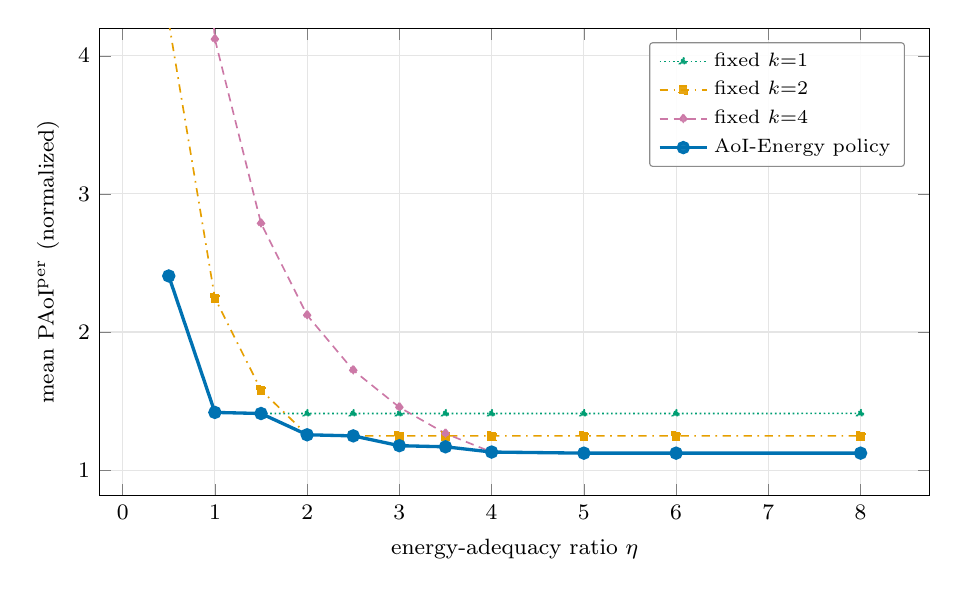
\begin{tikzpicture}
\begin{axis}[paperfig,width=\columnwidth,height=0.62\columnwidth,
  xlabel={energy-adequacy ratio $\eta$},ylabel={mean $\PAoIper$ (normalized)},
  legend pos=north east,grid=both,legend cell align=left,ymax=4.2]
\addplot[cC,semithick,densely dotted,mark=triangle*,mark size=1.5pt] coordinates {(0.5,2.406) (1.0,1.418) (1.5,1.410) (2.0,1.410) (2.5,1.410) (3.0,1.410) (3.5,1.410) (4.0,1.410) (5.0,1.410) (6.0,1.410) (8.0,1.411)};
\addlegendentry{fixed $k{=}1$}
\addplot[cE,semithick,dashdotted,mark=square*,mark size=1.5pt] coordinates {(0.5,4.244) (1.0,2.246) (1.5,1.580) (2.0,1.256) (2.5,1.248) (3.0,1.248) (3.5,1.248) (4.0,1.248) (5.0,1.248) (6.0,1.248) (8.0,1.248)};
\addlegendentry{fixed $k{=}2$}
\addplot[cD,semithick,densely dashed,mark=diamond*,mark size=1.6pt] coordinates {(0.5,8.111) (1.0,4.121) (1.5,2.787) (2.0,2.122) (2.5,1.723) (3.0,1.455) (3.5,1.265) (4.0,1.131) (5.0,1.123) (6.0,1.123) (8.0,1.123)};
\addlegendentry{fixed $k{=}4$}
\addplot[cA,very thick,mark=*,mark size=1.8pt] coordinates {(0.5,2.406) (1.0,1.418) (1.5,1.410) (2.0,1.256) (2.5,1.248) (3.0,1.177) (3.5,1.169) (4.0,1.131) (5.0,1.123) (6.0,1.123) (8.0,1.123)};
\addlegendentry{AoI-Energy policy}
\end{axis}
\end{tikzpicture}
\caption{Mean $\PAoIper$ of each fixed replication degree and of the
two-candidate rule \eqref{eq:policy} versus the energy adequacy $\eta$
($B{=}64$, $K_{\max}{=}4$; eight seeds, shared across $k$). The rule
matched the per-$\eta$ exhaustive optimum at all $11$ energy levels and
is the lower envelope of the fixed-degree curves.}
\label{fig:policy}
\end{figure}

% AUTO-GENERATED by figs/make_figures.py -- do not edit.
\begin{figure}[t]\centering
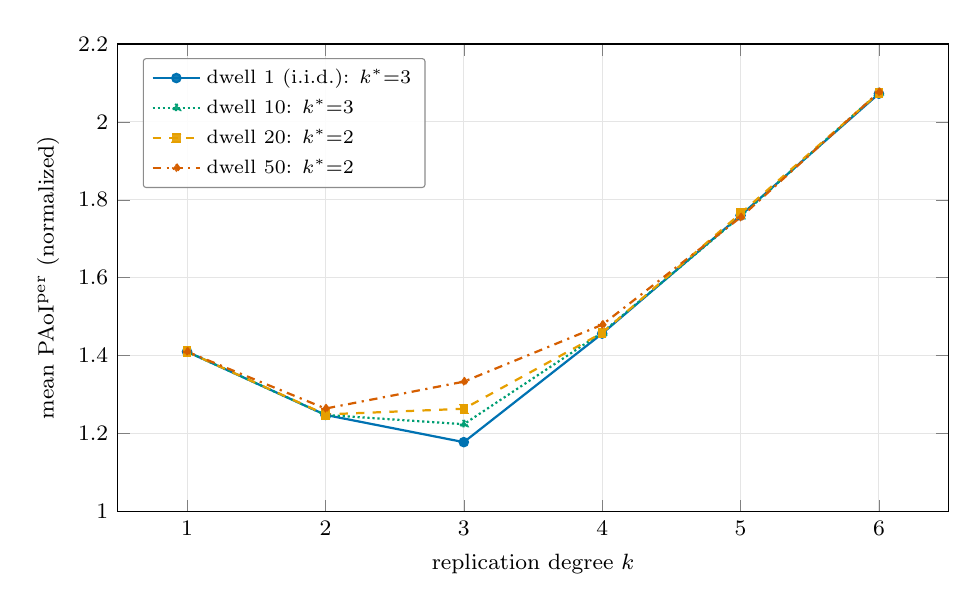
\begin{tikzpicture}
\begin{axis}[paperfig,width=\columnwidth,height=0.62\columnwidth,
  xlabel={replication degree $k$},ylabel={mean $\PAoIper$ (normalized)},
  legend pos=north west,grid=both,legend cell align=left,xtick=data,
  ymin=1.0,ymax=2.2]
\addplot[cA,thick,solid,mark=*,mark size=1.5pt] coordinates {(1,1.4101) (2,1.2478) (3,1.1779) (4,1.4566) (5,1.7600) (6,2.0726)};
\addlegendentry{dwell $1$ (i.i.d.): $k^\ast{=}3$}
\addplot[cC,thick,densely dotted,mark=triangle*,mark size=1.5pt] coordinates {(1,1.4102) (2,1.2478) (3,1.2239) (4,1.4593) (5,1.7577) (6,2.0762)};
\addlegendentry{dwell $10$: $k^\ast{=}3$}
\addplot[cE,thick,dashed,mark=square*,mark size=1.5pt] coordinates {(1,1.4102) (2,1.2490) (3,1.2636) (4,1.4584) (5,1.7649) (6,2.0748)};
\addlegendentry{dwell $20$: $k^\ast{=}2$}
\addplot[cB,thick,dashdotted,mark=diamond*,mark size=1.5pt] coordinates {(1,1.4102) (2,1.2641) (3,1.3332) (4,1.4792) (5,1.7549) (6,2.0765)};
\addlegendentry{dwell $50$: $k^\ast{=}2$}
\end{axis}
\end{tikzpicture}
\caption{Measured failure boundary of the mean-based set-point under
bursty harvest (E15; $\eta{=}3$, $K_{\max}{=}6$, $B{=}64$;
two-state Markov-modulated harvest with the stated mean dwell, twelve
seeds). The $\PAoIper(k)$ curve keeps its minimum at
$k^\ast{=}3{=}\lfloor\eta\rfloor$ up to a mean dwell of ten periods;
from a dwell of $20$ periods the minimum moves to $k{=}2$ and stays
there through dwell $100$ (not shown), because long lean spells make the
third copy's starvation cost exceed its order-statistic gain. The
work-conservation identity holds at every dwell ($\le3.1{\times}10^{-4}$).}
\label{fig:e15}
\end{figure}


\paragraph*{Worked example (Iridium-class numbers)}
Take our LEO scenario S1: $P=5736$\,s, $W=430$\,s
($\delta=0.075$), $T_s=10$\,s, and a solar harvest that accumulates one
copy's energy every $2200$\,s, so $\eta=\lambda_e P/e=2.6$. Suppose the
battery is large and CGR offers at least three satellites of this
period and window whose pass phases are unknown to the source at
decision time (plan model~(i)). The two candidates are $k\in\{2,3\}$; the ceiling test \eqref{eq:ceiltest}
compares added starvation $P(3/2.6-1)=882$\,s against order-statistic
gain $g_2-g_3=463$\,s, so the floor wins: $k_{\mathrm{pol}}=2$. The
resulting mean $\PAoIper$ is $P+\E[R_{\min,2}]+T_s=5736+1513+10\approx
7.3\times10^3$\,s ($\approx 2.0$\,h), versus $8.2\times10^3$\,s
($\approx2.3$\,h) single-copy, a $12\%$ freshness gain for one extra
copy, whereas $k{=}3$ would \emph{lose} ground
($\mathcal{A}(3)-\mathcal{A}(2)\approx+419$\,s) by starving one window in
$7.5$. The gain is the phase-agnostic one: were the pass phases known
and the routes reliable, a single copy on the earliest route would tie
(Remark~\ref{rem:uncertainty}).

\paragraph*{Tail and deadline-violation probability}
For mission-critical traffic the relevant quantity is the
\emph{tail} $\Pr(\PAoIper>d)$ at a deadline $d$, not the mean, and in
the LEO $k$-copy model the tail is available in closed form.

\begin{corollary}[$\PAoIper$ tail, LEO $k$-copy]\label{cor:tail}
Under the model of Section~\ref{sec:r3} with i.i.d.\ firing (exact when
$\peff=1$; mean-field otherwise), the per-update peak decomposes as
$\PAoIper=JP+R_{\min,k}+T_s$ with $J\sim\mathrm{Geom}(\peff)$ independent of
$R_{\min,k}$. Write the deadline as $d=T_s+jP+r$ with $j\ge1$ the
integer number of whole periods and $r\in[0,P)$ the remainder; then
\begin{equation}\label{eq:tailcf}
\begin{aligned}
\Pr(\PAoIper>d)&=(1-\peff)^{j}\\
&\quad+\peff(1-\peff)^{j-1}\Bigl(\tfrac{G-r}{P}\Bigr)^{k}\ind\{r\le G\},
\end{aligned}
\end{equation}
and in the energy-abundant regime ($\peff{=}1$) the $\beta$-quantile is
$T_s+P+\max\bigl\{0,\;G-P(1-\beta)^{1/k}\bigr\}$: the maximum handles the
atom of $R_{\min,k}$ at $0$ (mass $1-(G/P)^k$, an update generated
inside a window), at which the quantile sits for all
$\beta\le1-(G/P)^k$.
\end{corollary}

Replication thus pulls the tail in polynomially, with exponent $k$.
The simulated complementary cumulative distribution function (CCDF;
Fig.~\ref{fig:ccdf}; twenty seeds, per-seed
quantiles) matches \eqref{eq:tailcf} pointwise. At a deadline of $1.5P$
the closed form gives $0.405^{k}=0.405,\,0.164,\,0.027$ for
$k{=}1,2,4$, against simulated $0.405\pm0.001$, $0.164\pm0.001$, and
$0.027\pm0.0003$: a $15.0\pm0.1\times$ reduction at $k{=}4$. The
reduction is not a feature of that one deadline: the per-seed ratio of
the single-copy to the four-copy violation probability rises
monotonically from $1.9\times$ at $d{=}1.1P$ through $7.7\times$ at
$1.4P$ to $35\times$ at $1.6P$ and $119\times$ at $1.7P$, as
$(G-r)^{3}$ dictates. The $99$th percentile $T_s+P+G-P(0.01)^{1/k}$
evaluates to $1.895P$ ($k{=}1$) and $1.589P$ ($k{=}4$), against
simulated $1.895\pm0.0001\,P$ and $1.589\pm0.001\,P$. For a renewal
segment the single-copy tail is immediate from \eqref{eq:renewal}:
$\Pr(\OPAoI>d)=\Pr(V>d-T_s)$. The mean alone therefore understates the
value of replication; the policy \eqref{eq:policy} extends to a deadline
constraint by minimizing $\mathcal{A}$ subject to
$\Pr(\PAoIper>d)\le\epsilon$, with the left side evaluated by
\eqref{eq:tailcf} rather than by simulation. Like the gain profile,
\eqref{eq:tailcf} is an average over the unknown firing phase
(Section~\ref{sec:model}).

% AUTO-GENERATED by figs/make_figures.py -- do not edit.
\begin{figure}[t]\centering
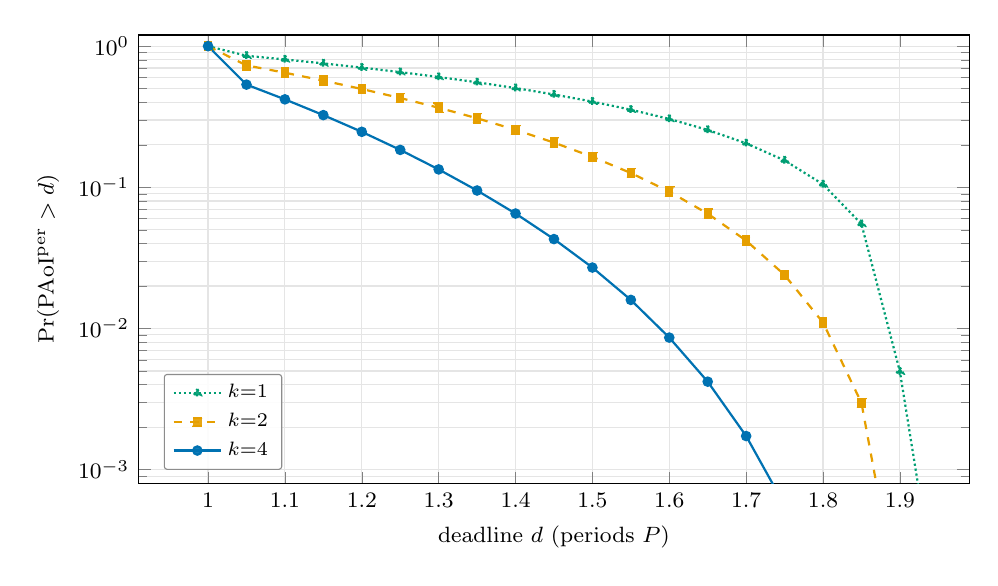
\begin{tikzpicture}
\begin{semilogyaxis}[paperfig,width=\columnwidth,height=0.6\columnwidth,
  xlabel={deadline $d$ (periods $P$)},
  ylabel={$\Pr(\PAoIper>d)$},legend pos=south west,grid=both,
  legend cell align=left,ymin=0.0008,ymax=1.2]
\addplot[cC,thick,densely dotted,mark=triangle*,mark size=1.5pt] coordinates {(1.0,1.00000) (1.05,0.85472) (1.1,0.80478) (1.15,0.75485) (1.2,0.70488) (1.25,0.65487) (1.3,0.60461) (1.35,0.55472) (1.4,0.50464) (1.45,0.45465) (1.5,0.40479) (1.55,0.35469) (1.6,0.30488) (1.65,0.25501) (1.7,0.20506) (1.75,0.15502) (1.8,0.10502) (1.85,0.05493) (1.9,0.00495) (1.95,0.00010) (2.0,0.00010)};
\addlegendentry{$k{=}1$}
\addplot[cE,thick,dashed,mark=square*,mark size=1.5pt] coordinates {(1.0,1.00000) (1.05,0.73084) (1.1,0.64828) (1.15,0.57018) (1.2,0.49706) (1.25,0.42926) (1.3,0.36631) (1.35,0.30839) (1.4,0.25535) (1.45,0.20744) (1.5,0.16429) (1.55,0.12629) (1.6,0.09323) (1.65,0.06507) (1.7,0.04193) (1.75,0.02394) (1.8,0.01101) (1.85,0.00297) (1.9,0.00010) (1.95,0.00010) (2.0,0.00010)};
\addlegendentry{$k{=}2$}
\addplot[cA,thick,mark=*,mark size=1.5pt] coordinates {(1.0,1.00000) (1.05,0.53407) (1.1,0.41990) (1.15,0.32474) (1.2,0.24722) (1.25,0.18416) (1.3,0.13392) (1.35,0.09492) (1.4,0.06522) (1.45,0.04298) (1.5,0.02702) (1.55,0.01594) (1.6,0.00862) (1.65,0.00420) (1.7,0.00173) (1.75,0.00056) (1.8,0.00012) (1.85,0.00010) (1.9,0.00010) (1.95,0.00010) (2.0,0.00010)};
\addlegendentry{$k{=}4$}
\end{semilogyaxis}
\end{tikzpicture}
\caption{$\PAoIper$ tail (deadline-violation probability) at
energy-abundant $\eta{=}6$ (twenty seeds; across-seed confidence intervals
below $10^{-3}$, invisible at this scale). Replication pulls the tail in
polynomially, with exponent $k$; the simulated points match the closed
form \eqref{eq:tailcf} pointwise (Section~\ref{sec:policy}).}
\label{fig:ccdf}
\end{figure}


\paragraph*{Comparison with a RUCoP-style MDP core}
RUCoP/CGR-UCoP casts routing under \emph{uncertain} contact plans as an
MDP that maximizes delivery probability for a copy budget. Rather than
reproduce the full CGR-UCoP pipeline, we implemented its decision core,
a RUCoP-style holder-set backward induction over the time-ordered
contacts that budgets transmissions and is validated against the closed
form $1-(1-q)^k$ on a symmetric plan. We solved it on one heterogeneous
uncertain diamond to obtain a delivery-versus-copies frontier (an
illustrative instance, not a benchmark-scale reproduction). The two
approaches are complementary. The MDP answers \emph{which} routes
maximize delivery and is energy-blind, so its optimum operates at the
budget ceiling $k{=}K_{\max}$; our policy answers \emph{how many}
copies the energy budget warrants. The frontier is concave, as it must be for
independent parallel routes taken in order of reliability, so copies
beyond the knee buy little delivery: at $k^\ast{=}2$ our policy
attains $94.7\%$ of the MDP's delivery for $40\%$ of the energy (the exact
percentages are instance-specific; the concavity, not the number, is the
point). The two compose: the MDP's route set under our degree cap is
the natural energy-aware extension of CGR-UCoP. Concretely, the
integration is: CGR (or CGR-UCoP) returns, per bundle, its candidate
routes ordered by best-case delivery time; the policy consumes the
first $k_{\mathrm{pol}}$ entries, or the $k_{\mathrm{pol}}$-subset chosen
by the phase-aware placement procedure when route-success estimates are
available; and RUCoP's holder-set computation, if used, is run with its
copy budget set to $k_{\mathrm{pol}}$ instead of to a confidence target.
Section~\ref{sec:sim} evaluates E-CGR, RUCoP, and both compositions
side by side on one instance.

\paragraph*{Robustness to contact-prediction error}
Contact plans are predictions. We model their reliability by the same
per-copy success probability $q$ as above: each committed copy's
predicted contact materializes w.p.\ $q$, with energy spent on the
commit regardless (a copy sent to a missed contact is wasted). A natural
intuition is to reserve energy under uncertainty and use $\lfloor
q\eta\rfloor$ copies. Our experiments show the opposite: the
PAoI-optimal degree stays at the no-starvation degree
$\lfloor\eta\rfloor$ for every $q\in[0.4,1]$ (here $\eta$ is set so
$\lfloor\eta\rfloor$ is the model optimum), because extra copies hedge
missed contacts through the order statistic over which copies
materialize. The rule therefore degrades gracefully ($+19\%$ $\PAoIper$ as $q$
falls to $0.4$), whereas the reserve heuristic under-replicates and is
counterproductive ($+50\%$ $\PAoIper$ at $q{=}0.4$). In the tested
regime, with independent per-copy materialization and energy spent
regardless, replication rather than a smaller copy budget is the right
response to prediction uncertainty; this is now also a
\emph{prediction} of Proposition~\ref{prop:uncertain} rather than only
an observation. With correlated failures, asymmetric route
probabilities, or route-dependent energy costs the optimal response can
differ, and the $q$-model would need the corresponding generalization
(experiment E19 in Section~\ref{sec:sim} tests the correlated-failure
case). The converse also deserves stating for deployments. Whether the
degree falls as uncertainty vanishes depends on the gain profile, which
must be that of the placement in use. Under phase-agnostic placement
the profile $g_k$ remains, and \eqref{eq:objq} at $q{=}1$ reduces to
\eqref{eq:obj}, whose minimizer still brackets $\eta$: unknown phases
are themselves uncertainty. Under plan-aware placement on CGR's
earliest routes the profile is instead the order-statistic one,
\begin{equation}\label{eq:hord}
h^{\mathrm{ord}}_k(q)=\frac{1}{s_k}\sum_{i=1}^{k}q(1-q)^{i-1}\,
\E\bigl[R_{(i)}\bigr],
\end{equation}
with $R_{(i)}$ the $i$-th smallest of the $K_{\max}$ candidate
residuals (the delivered copy is the earliest survivor). At $q{=}1$
this profile is flat in $k$, so all degrees up to $\lfloor\eta\rfloor$
tie and a single copy is energy-optimal, the oracle tie of
Remark~\ref{rem:uncertainty}; at $q{=}2/3$ it selects the
same degree as \eqref{eq:policy} at every energy level of the
matched-budget experiment of Section~\ref{sec:sim}. Better prediction
of both outcomes and phases is thus a substitute for replication,
provided the objective is evaluated with the profile of the placement
in use.

% =====================================================================
\section{Numerical Validation}\label{sec:sim}
Validation follows a two-tier plan, closed by a reference-implementation
cross-check, on the reference scenarios S1--S3 of
Section~\ref{sec:model}. Tier~1 is \emph{model-exact}: a Monte Carlo
simulator that implements the stochastic model of
Section~\ref{sec:model} directly (gating, batteries, copies, and
faults exactly as specified, with no protocol stack), so a discrepancy
with a closed form isolates a derivation error rather than a protocol
effect. It confirms the closed forms over the parameter sweeps (duty
cycle $\delta$, replication degree $k$, energy adequacy $\eta$, battery
capacity $B$). Tier~2 is \emph{DTN-realistic}: a stack with Bundle
Protocol and Contact Graph Routing (\texttt{dtnsim}~\cite{fraire2017dtnsim},
the public contact-plan simulator of the RUCoP/CGR-UCoP lineage), extended with a custom
energy-harvesting battery module and a CGR-native $k$-copy router, runs
the representative scenarios and compares single-copy CGR against CGR
replication under an energy budget; a discrepancy there can also come
from the stack (route recomputation, convergence-layer timing). E-CGR-
and RUCoP-style decision rules are reimplemented and compared in the
Tier-1 harness below, and a RUCoP-style MDP core is compared on an
illustrative instance in Section~\ref{sec:policy}. Each theoretical
claim maps to one experiment with a quantitative pass criterion: the
mixed residual law and the quadratic-mean/linear-peak divergence of
Theorem~\ref{thm:r1}; the fixed-plan mixing approximation and its
phase-locking failure mode (Remark~\ref{rem:fixedmix}); the
Gini-dispersion replication gain and its collapse for same-bottleneck
copies (Theorem~\ref{thm:r2}); the unimodal objective and threshold
$\kstar$ with monotonicity and saturation (Theorem~\ref{thm:r3}); and
the work-conservation firing fraction with the finite-battery correction
and its downward pressure on $\kstar$ (Lemma~\ref{lem:work}).

\paragraph*{Software, seeds, and hardware}
Tier~1 is a stdlib-only Python simulator (Python 3.10--3.12 tested in
continuous integration; no third-party packages). Tier~2 uses the public dtnsim (\url{github.com/lggaray/dtnsim}, commit
\texttt{a9cf3fc6}) on OMNeT++~5.7.1, with our energy
module and $k$-copy router applied as patches shipped with the artifact.
Contact plans are static ION-format plans (one \texttt{a contact} line
per window with start, end, endpoints, and rate); CGR (dtnsim's
\texttt{cgrModel350}) computes routes per bundle at its forwarding event
and recomputes when a fault blocks the chosen next hop; relay faults are
dtnsim's native exponential ON/OFF process (S2). Real-ephemeris plans
are propagated with Skyfield~1.48 from CelesTrak two-line elements whose
SHA-256 is recorded in the artifact. The ION cross-check ran
ION-DTN~4.1.4 (BPv7) with two nodes on one Ubuntu~24.04 LTS virtual
machine (Intel Core i9-12900K host, User Datagram Protocol (UDP)
convergence layer over loopback), so the reported dispatch lag is a
software quantity, not a radio one. Seeds are fixed in each script, so
every reported simulation number can be regenerated from the artifact
(bit for bit on the same Python minor version; the ION run, which
executes in real time, is reproducible only statistically), and the
Tier-2 raw result files record the seed of each run. Seed counts are
$8$--$20$ for the Tier-1 sweeps (the measured firing fractions reported
with E11 come from one seed) and, for Tier~2, ten for the two-relay,
unified, and heterogeneous-chain experiments, five for the atomic
experiment, and three for the capacity experiment; the Tier-2
residual-law, relay, renewal, and ephemeris results and the ION run are
single runs on one contact plan each. The repository README documents
installation, environment setup, and the command that regenerates each
figure, and a frozen copy of the reported dataset ships alongside for
comparison.

\paragraph*{Statistical conventions}
Each reported mean from a multi-seed experiment is the across-seed mean
of independent replications. An interval quoted after $\pm$ is a $95\%$
Student-$t$ confidence interval (CI) over seeds unless it is stated to
be a standard deviation.
Curves compared across degrees $k$ (e.g.\ Fig.~\ref{fig:policy}) use
the same seed set for every $k$, so differences between curves are
paired. ``Matches to $x\%$'' denotes the maximum, over the sweep, of the
relative absolute difference $|\text{simulated}-\text{model}|/\text{model}$
between the across-seed mean and the closed form; each experiment's
pass criterion is stated in its script and in the artifact's validation
matrix (for example, $2\%$ for the uncertainty objective). Seed counts
were not derived from a power calculation; the precision they achieved
is as follows. Intervals are recorded for the
residual-law sweeps (half-width at most $0.13\%$ of the mean), for the
work-conservation, matched-budget, adaptive-baseline, route-set, and
CGR-family experiments (at most $0.6\%$), for the bursty-fault
experiment (at most $1.2\%$), and for the tail and order-preservation
experiments (Fig.~\ref{fig:ccdf}). The remaining Tier-1 experiments
record across-seed means only, among them the policy, threshold,
ceiling, finite-battery, bursty-harvest, renewal, uncertainty,
phase-mixing, and two-copy-gain sweeps; their conclusions are locations of minima or agreements
with closed forms, and in the policy sweep the optimum is separated
from the runner-up by at least $3.3\%$ of the mean, well above the
intervals of the comparable experiments. For Tier~2, half-widths are at
most $1.2\%$ in the unified and atomic experiments; the two-relay
comparison is reported through paired per-seed differences, and the
capacity experiment, which has three seeds, through per-seed ratios.
Quantiles are across-seed means of per-seed quantiles with their own
interval.

\paragraph*{Tier-1 results}
Table~\ref{tab:tier1} is the audit trail of the first tier: each row
names an analytical claim, the statistic its experiment computes, and
the outcome against the pass criterion (time normalized to $P{=}1$;
seed counts and conventions as above). All rows pass, and the text
discusses only those whose outcome is more than a plain match. The
\emph{ceiling} branch flips exactly at the analytic crossover of
\eqref{eq:ceiltest} ($\delta{=}0.1$ on $[3,4]$: simulated flip between
$\eta{=}3.8$ and $3.9$, $\eta^\star{=}3.824$), so the extra copy is
taken precisely when its gain repays the added starvation. The
bursty-harvest row is the policy's measured \emph{failure boundary}
(Fig.~\ref{fig:e15}): the threshold and the work-conservation identity
survive Markov-modulated harvest up to a mean dwell of ten periods
(correlation moves the 99th percentile at $\kstar$ from $1.78P$ to
$3.07P$, the Markov-renewal effect anticipated in
Section~\ref{sec:r3hard}), but from
a mean dwell of $20$ periods the optimum retreats to $k{=}2$ and stays
there through dwell $100$ (by a margin of $1.2\%$ at dwell $20$, growing
to $5.5\%$ at dwell $50$ and $7.5\%$ at dwell $100$; these sweeps record
means only), the regime where a mean-based set-point
should yield to regime-aware adaptation (cf.\
Section~\ref{sec:policy}).

\begin{table}[t]
\caption{Tier-1 traceability: analytical claim $\to$ model-exact check.}
\label{tab:tier1}
\centering
\renewcommand{\arraystretch}{1.18}
\setlength{\tabcolsep}{3pt}
\footnotesize
\begin{tabular}{>{\raggedright\arraybackslash}p{0.24\columnwidth}>{\raggedright\arraybackslash}p{0.315\columnwidth}>{\raggedright\arraybackslash}p{0.315\columnwidth}}
\hline
Claim & Check & Outcome \\
\hline
Residual law, Thm~\ref{thm:r1} & KS to mixed law; mean/peak exponents in $(1{-}\delta)$ & KS $0.002$; slopes $1.98/1.00$ (Fig.~\ref{fig:r1}) \\
Fixed-plan mixing, Rem.~\ref{rem:fixedmix} & phase KS-to-uniform, corr.; commensurate control & $0.001$, $|\text{corr.}|{=}0.002$; locked: KS $0.89$ \\
Two-copy gain, Thm~\ref{thm:r2} & Gini identity; ratio $\tfrac23(1{-}\delta)$; same-bottleneck & matched (Fig.~\ref{fig:r2gain}); zero gain \\
Threshold, \eqref{eq:kstar}, Thm~\ref{thm:r3} & unimodality; staircase, saturation & argmin brackets $\eta$ (Figs.~\ref{fig:r3unimodal},~\ref{fig:r3kstar}) \\
Ceiling branch \eqref{eq:ceiltest} & fine $\eta$-sweep on $[3,4]$ & flip at $\eta^\star{=}3.824$ \\
Work cons., Lem.~\ref{lem:work} & $k\peff{=}\eta{-}L$; $k{=}1$ P--K law; Poisson vs.\ deterministic & $\le\!1.2{\times}10^{-4}$; distribution-free; $\peff(1){=}\eta$ \\
Finite $B$, Sec.~\ref{sec:r3hard} & $\kstar$ vs.\ $B$ (E11); exact chain & $4\to2$ as $B$: $64\to4$ ($\eta{=}4$); chain reproduces every point \\
Bursty harvest (E15) & Markov-modulated dwell sweep, $\eta{=}3$ & $\kstar$ invariant to dwell $10$; wc $\le\!3.1{\times}10^{-4}$; $k{=}2$ from dwell $20$ (Fig.~\ref{fig:e15}) \\
Renewal laws \eqref{eq:renewal},\newline\eqref{eq:invcond} & det., jitter, exp., Pareto; inversion threshold & $\E[R]$ within $1\%$; crossing matched (Fig.~\ref{fig:inversion}) \\
Uncertainty, Prop.~\ref{prop:uncertain} (E18) & \eqref{eq:objq} vs.\ sim over $q{\times}k{\times}\eta$ & within $0.7\%$; optimum equals the rule's choice \\
Bursty faults (E19) & Markov route faults, dwell $1.5$--$75$ & means move $<1.3\%$; optimum in or tied with candidate set \\
Order preservation (E20) & S3 chain, first-in-first-out segments, two cadences & zero inversions (structural); $\E[Z]{+}\E[Y]$ exact to $0.03\%$ \\
\hline
\end{tabular}
\end{table}

\paragraph*{Tier-2 results (DTN-realistic CGR)}
We reproduce the findings in dtnsim, a Bundle Protocol / Contact Graph
Routing simulator of the CGR lineage, over the same scenarios with a
custom energy-harvesting battery module. Result~1: routing periodic
status updates over a real contact plan yields a mean delivery delay of
$2453.9$\,s against the closed-form $\E[R]{=}2454.1$\,s, and the
delay histogram reproduces the full mixed residual law (atom plus uniform
slab). Result~2: for a two-segment relay, the end-to-end latency standard
deviation matches $\sqrt{\operatorname{Var}R_1+\operatorname{Var}R_2}$
under incommensurate segment periods (independence) but collapses toward
$\sqrt{\operatorname{Var}R_1}$ under commensurate periods (phase locking),
supporting the fixed-plan mixing approximation of
Remark~\ref{rem:fixedmix} and demonstrating its phase-locking failure
mode (the random-offset mixing property remains the exact
result). The renewal residual
law \eqref{eq:renewal} holds within $0.5\%$ across gamma contact-gap
laws with $\mathrm{CV}$ of $0.48$, $1.04$, and $1.88$, and the AoI/PAoI
inversion (Remark~\ref{rem:inversion}) is absent at the two lower values
and present at the highest, consistent with \eqref{eq:invcond}; this
grid is too coarse to locate the threshold, which the Tier-1 sweep does
(Fig.~\ref{fig:inversion}). Result~3, starvation side: the threshold's
over-replication penalty is validated in the DTN stack with
\emph{update-atomic} all-or-nothing admission (launch $k$ copies iff
the battery holds $k$ units, else skip the whole update) on a
fault-free three-relay staggered diamond with a six-copy source battery
(Fig.~\ref{fig:r3atomic}).
With one update every $\GEN{=}1.062P$, admitted fractions match
$\min\bigl(1,\eta\,\GEN/(kP)\bigr)$ to within $0.7\%$ at every
$(\eta,k)$, and over-replication is punished as \eqref{eq:obj}
predicts: at $\eta{=}1$, $k{=}3$ skips two of three updates and its
peak age is $2.7\times$ single-copy's. The same experiment exhibits
Remark~\ref{rem:uncertainty} in dtnsim's CGR: fault-free, higher
degrees \emph{tie} (never strictly win) once $\eta\ge k$.

% AUTO-GENERATED by figs/make_figures.py -- do not edit.
\begin{figure}[t]\centering
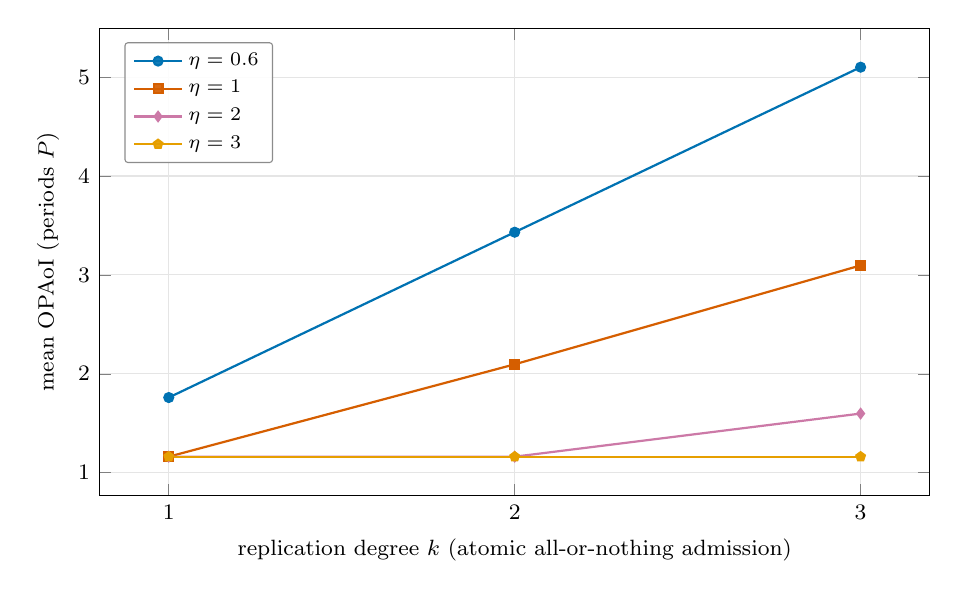
\begin{tikzpicture}
\begin{axis}[paperfig,width=\columnwidth,height=0.62\columnwidth,
  xlabel={replication degree $k$ (atomic all-or-nothing admission)},
  ylabel={mean OPAoI (periods $P$)},legend pos=north west,grid=both,
  legend cell align=left,xtick={1,2,3}]
\addplot[thick,cA,mark=*,mark size=1.6pt] coordinates {(1,1.760) (2,3.432) (3,5.101)};
\addlegendentry{$\eta=0.6$}
\addplot[thick,cB,mark=square*,mark size=1.6pt] coordinates {(1,1.162) (2,2.096) (3,3.096)};
\addlegendentry{$\eta=1$}
\addplot[thick,cD,mark=diamond*,mark size=1.6pt] coordinates {(1,1.162) (2,1.162) (3,1.598)};
\addlegendentry{$\eta=2$}
\addplot[thick,cE,mark=pentagon*,mark size=1.6pt] coordinates {(1,1.162) (2,1.162) (3,1.162)};
\addlegendentry{$\eta=3$}
\end{axis}
\end{tikzpicture}
\caption{Tier-2 atomic threshold test (dtnsim CGR, fault-free
three-relay staggered diamond; update-atomic admission launches $k$
copies iff the battery holds $k$ units and otherwise skips the whole
update; five seeds). Over-replication is penalized as \eqref{eq:obj}
predicts: at $\eta{=}1$, $k{=}3$ admits $35\%$ of updates and its
peak age is $2.7\times$ single-copy's. At $\eta\ge3$ the degrees tie,
because on a fault-free plan CGR's single copy already rides the
earliest route (Remark~\ref{rem:uncertainty}).}
\label{fig:r3atomic}
\end{figure}


\paragraph*{Two-relay plan under faults}
On the two-relay instance of S2, with relay faults and a
per-transmission source energy gate, updates are generated every
$\GEN{=}300$\,s (about $19$ per period), so the energy axis is the
adequacy per update, $\eta_{\mathrm{g}}=\lambda_e\GEN/e$, not the
per-period $\eta$ of Section~\ref{sec:r3}. Against dtnsim's stock
single-copy router, our $k$-copy router at $k{=}2$ gives a mean $\OPAoI$
$5.9$--$6.5$ times lower at every energy level when the source battery
holds five copies. A controlled comparison (ten seeds, our router in
both arms at one and two copies, source batteries of five and $32$
copies) shows that this ratio is not a hedging gain. With the same
router the single-copy results are identical, seed for seed, to the
stock router's ($8.9P$ at $\eta_{\mathrm{g}}{=}0.6$), so the router is
not the cause. With the $32$-copy battery the energy levels fall into
three cases. At $\eta_{\mathrm{g}}{=}1.5$ and $2$, below the two copies'
energy demand, two copies are staler by $0.49P$ and $0.46P$ (paired
per-seed differences, $95\%$ CIs excluding zero): the starvation side
of the threshold. At $\eta_{\mathrm{g}}{=}3$ and $6$, where energy
suffices, a single copy at $0.71P$ is as fresh as two or fresher (by
$0.15\pm0.14P$ and $0.05\pm0.11P$). Only at the lowest level,
$\eta_{\mathrm{g}}{=}0.6$, and with the five-copy battery does the large
ratio remain; there the source cannot keep up with its own updates,
delivery is incomplete in both arms, and the ratio reflects a standing
backlog rather than the order-statistic hedge. The absence of a hedge
has a structural cause in this plan. Each relay's uplink and downlink
contacts share the same windows (a bent pipe), so a faulted relay
almost never holds a committed bundle; the bundle waits at the source,
CGR re-routes it, and a single copy already attains the minimum over
the relays. This is the $q\to1$ limit of \eqref{eq:hord}, not the
fault-free oracle tie, and exhibiting a hedge in the stack would need a
plan in which a stall strands a copy already in flight. We report this
experiment in the text only (\texttt{run\_r3\_cgr\_control.sh}); the
hedge as a function of the per-pass success $q$ is computed
model-exactly in the matched-budget comparison below.

\paragraph*{Unified experiment: one topology, one admission rule, both
metrics}
Because the preceding experiments varied the metric and the admission
mechanism together with the question, we close Tier-2 with a single
experiment holding everything fixed: the three-relay staggered diamond
with a six-copy source battery, update-atomic all-or-nothing admission, relay faults \emph{on}
(availability $2/3$), sweeping $k\in\{1,2,3\}\times
\eta\in\{1,2,3,6\}$ ($10$ seeds) and reporting $\OPAoI$, per-update
$\PAoIper$, mean delay, delivered/admitted counts, and energy per
update ($=ke$) side by side. The two peak metrics agree on every
ordering. The starvation side is large and statistically unambiguous:
every degree above $\eta$ is penalized ($k{=}3$ at $\eta{=}1$: $+144\%$;
$k{=}2$ at $\eta{=}1$: $+71\%$; $k{=}3$ at $\eta{=}2$: $+33\%$), so the
freshness-optimal degree is at most $\lfloor\eta\rfloor$ at every energy
level. Among the degrees that energy affords, the means are ordered as
the theory predicts ($-0.6\%$ and $-0.8\%$ for the second copy in
$\OPAoI$ and $\PAoIper$, and a further $-0.2$ to $-0.3\%$ for the
third), but the paired
per-seed differences are within noise ($-44\pm131$\,s for the second
copy and $-16\pm98$\,s for the third, against a mean of
$7.4\times10^{3}$\,s). The experiment is therefore consistent with
$\min(K_{\max},\lfloor\eta\rfloor)$ without resolving it. The reason
the hedge is small is itself informative: dtnsim's faults are
\emph{stall-type} (a faulted relay pauses, CGR re-routes, no bundle is
lost; delivery stays $100\%$), and in this three-relay staggered plan
re-routing recovers most stalls, so the hedge shrinks to the few updates
that a fault strands mid-pass. The value of replication is set by how
often a fault becomes a per-pass loss given the plan's
alternatives, that is, by the effective $q$ of
Proposition~\ref{prop:uncertain}, which is close to one here. Tier~2
thus corroborates the starvation side of the threshold.

\paragraph*{Real ephemeris: residual law and phase alignment}
Replacing the synthetic LEO schedule with a contact plan generated from
real Iridium-NEXT ephemeris (propagated over a polar ground station;
cf.\ polar-coverage constellation design~\cite{ma2026igso}) reproduces
the renewal residual law to within $0.1\%$ for the reference satellite
($2490.9$\,s versus the predicted $2492.4$\,s over $101$ passes).
Extending the ephemeris study to satellite \emph{pairs} instantiates
the plan-model taxonomy of Section~\ref{sec:r3} on real orbits.
Scanning $40$ Iridium-NEXT companions of the reference satellite over
the same station, we find that the route-set \emph{latency-diversity
potential}, the residual-min ratio $\E[R_{\min,2}]/\E[R_1]$, spans
$0.41$ to $0.95$ with the pair's
pass-phase alignment, tracing the phase ladder \eqref{eq:ladder}: an
anti-phased pair (residual correlation $-0.51$, plan model (ii)) beats
the ensemble reference of $\tfrac23(1-\delta){=}0.61$; the best
near-independent pair (correlation $0.07$, plan model (i)) matches the
product form \eqref{eq:rminprod} within $4.3\%$, the other
near-independent pairs within $5$--$7\%$; and a phase-locked pair
(correlation $+0.88$, plan model (iii)) raises the ratio to $0.95$. The
mean over the $40$ pairs is $0.61$, the ensemble reference. This is not
a realized replication gain (Remark~\ref{rem:uncertainty}); the scan
measures the \emph{diversity that replication converts into freshness
once route outcomes are uncertain}. Two lessons stand. The dependence of
fixed-plan residuals on a common arrival instant is a measured
phenomenon on operational constellations, not a technicality; and
because contact plans are known in advance, the phase alignment of candidate routes is \emph{computable
at planning time} via \eqref{eq:rminjoint}, which is the basis of the
phase-aware placement procedure of Section~\ref{sec:policy}.

\paragraph*{Matched-budget baseline comparison}
To place the policy against its routing-family baselines under the
\emph{same} copy budget ($K_{\max}{=}3$), the same battery/harvest
process ($B{=}12$, sweep over $\eta$), and the same route selection
(all schemes commit copies to the plan-earliest routes; only the
\emph{degree} differs), we run the model-exact simulator with a
per-pass route success $q{=}2/3$ on every route, that is, with
loss-type faults. Numerically this is the availability of the Tier-2
relays, but it is not the effective $q$ of dtnsim's stall-type faults,
which is close to one (above); the experiment therefore shows the hedge
as a function of $q$, not the hedge of the Tier-2 scenarios. We compare the
two-candidate $\kstar(\eta)$ with two baselines: earliest-arrival
single-copy CGR (in our single-energy-bottleneck
abstraction, E-CGR's battery validation~\cite{ecgr} coincides with the
energy gate, so the gated $k{=}1$ baseline \emph{is} the E-CGR-style
policy) and RUCoP-style delivery-max replication (energy-blind,
$k{=}K_{\max}$ always). Three
regimes emerge (mean $\PAoIper$ in units of $P$, $10$ seeds, $95\%$
CIs below $\pm0.04$): energy-scarce ($\eta\le1.5$), $\kstar{=}1$ and
the policy \emph{equals} single-copy CGR ($3.14$ at $\eta{=}0.5$)
while delivery-max over-replicates catastrophically ($6.47$,
$2.1\times$ worse); transition ($\eta{=}2$--$2.5$), the policy
strictly dominates both ($1.375$ vs.\ $1.640$ / $1.785$ at
$\eta{=}2$); energy-abundant ($\eta\ge3$), the policy coincides with
full diversity ($1.32$) while single-copy stays fault-limited
($1.64$). The same harness also tests Remark~\ref{rem:uncertainty}
and the phase ladder jointly: on a two-route plan with $q{=}1$ (no
faults), single-copy CGR \emph{ties} $k{=}2$ within CI for every plan
structure (locked, independent, anti-phased), by construction in this
harness, where the single copy rides the earlier of the two routes (the
non-trivial instance of the tie is the Tier-2 atomic experiment);
whereas at $q{=}2/3$
the two-copy set reduces mean $\PAoIper$ by $16$--$20\%$ with the
predicted ordering
anti ($1.378$) $<$ independent ($1.418$) $<$ locked ($1.497$).
Three \emph{battery-state-adaptive} rules complete the baseline set:
battery-greedy (fire $\min(K_{\max},\lfloor b\rfloor)$ copies each
epoch); earliest-$K$ (replicate to the earliest $K_{\max}$ routes
whenever the battery affords it, else a single copy); and floor-greedy,
the simplest energy-constrained rule (fire $\lfloor\eta\rfloor$ copies
when affordable, else whatever the battery holds). The mean-based
set-point dominates greedy and earliest-$K$ wherever energy binds, by
up to $29\%$ over greedy at $\eta{=}1$ ($1.70$ vs.\ $2.20$), where
adaptive rules over-spend scarce harvest; floor-greedy equals it
there (both fire one copy per affordable epoch). In the transition and
energy-abundant regimes the partial-firing rules edge the set-point:
floor-greedy by $1.4\%$ at $\eta{=}2$ ($1.356$ vs.\ $1.375$), and greedy
and earliest-$K$ by $2.7\%$ and $2.5\%$ at $\eta{=}3$ ($1.286$ and
$1.289$ vs.\ $1.321$), because with faults present firing a
\emph{partial} degree beats the occasional all-or-nothing skip. The
all-or-nothing restriction, not the two-candidate degree, is what these
rules exploit; relaxing it is a natural refinement, and in this
configuration its price is the $1.4$--$2.7\%$ above. The
uncertainty-aware objective itself is validated model-exactly (E18):
simulated mean $\PAoIper$ matches \eqref{eq:objq} within $0.7\%$ over
$q\in\{0.4,0.7,1\}\times k\le4$ at $\eta\in\{3,6\}$, and the simulated
optimum equals the rule's choice in every case. These integer-$\eta$
cases do not exercise the ceiling branch under $q<1$, which the grid
computation of Section~\ref{sec:r3} covers. Scenario and
outputs ship with the artifact (\texttt{e\_baselines.py},
\texttt{e18\_uncertain.py}).

\paragraph*{CGR-family comparison: E-CGR, RUCoP, and their compositions}
How does the degree rule fare against the published energy-aware and
uncertainty-aware CGR decision rules themselves? We reimplemented both
in the matched-budget harness (Fig.~\ref{fig:cgrfamily}; $K_{\max}{=}4$
candidate routes with \emph{heterogeneous} per-route success
$q_i\in\{0.90,0.75,0.60,0.45\}$ and ensemble phases, so timing diversity
and failure diversity no longer coincide; $B{=}12$; ten seeds).
\emph{E-CGR}~\cite{ecgr}: CGR's candidate routes in earliest-arrival
order are validated against the energy state (a transmission must
leave the battery at or above a reserve), and the first route that
passes carries one copy; if none passes the bundle is held, which under
paced generation means the held update is superseded by the next (we
report reserves of $0$ and $1$ copy; they differ by $<0.5\%$).
\emph{RUCoP}~\cite{rucop}: the holder-set MDP core of
Section~\ref{sec:policy} with its budget at $K_{\max}$
(delivery-optimal, energy-blind), committing to the most reliable
routes. \emph{RUCoP set $+$ degree cap}: RUCoP's route set under
$k^{\ast}(\eta)$. \emph{Ours}: $k^{\ast}(\eta)$ copies on the $k^{\ast}$
earliest routes (CGR order, as realized by our router). \emph{Ours $+$
phase-aware placement}: $k^{\ast}(\eta)$ with the per-bundle subset rule
of Section~\ref{sec:policy}. On this single-hop diamond with one source
battery both published rules simplify, and we say so plainly. E-CGR's
per-node energy validation reduces to a reserve-gated single copy on
CGR's earliest route: all routes draw the same battery, so validation
never reorders them. RUCoP's holder-set optimization reduces to
committing its budget to the most reliable routes; we run the MDP only
to confirm that reduction. The comparison therefore isolates the degree
and placement decisions of each rule, not their multi-hop machinery. An
instance in which E-CGR's per-relay validation and RUCoP's holder sets
are non-trivial needs per-relay batteries, which our energy model does
not have. Three findings emerge. First, E-CGR coincides
with the degree rule wherever $k^{\ast}{=}1$ (it \emph{is} the
energy-validated single copy) and is left behind once energy affords a
second copy (E-CGR stays at $1.55$, against $1.30$ at $\eta{=}2$ and
$1.24$ at $\eta{=}3$ for the degree rule). Second, energy-blind RUCoP is $2.7\times$ worse than E-CGR
at $\eta{=}0.5$ and meets the rule only at $\eta\ge K_{\max}$, while
RUCoP's route set under the degree cap already recovers most of that
loss. At $k^{\ast}{=}1$ its most reliable route even \emph{beats} CGR's
earliest route ($1.53$ versus $1.61$ at $\eta{=}1$): with a single copy,
failure diversity outweighs timing. Third, the per-bundle phase-aware
placement is the best scheme, or tied for best, at every energy level
($1.45$ at $\eta{=}1$ and $1.27$ at $\eta{=}2$; at $\eta{=}3$ its margin
over the degree rule is $0.3\%$, and from $\eta{=}4$, where every
replicating scheme commits all four routes, they coincide) because it
prices both diversities per update; a planning-time \emph{fixed} set
cannot,
since under ensemble phases it reduces to the reliability ranking, i.e.\
to RUCoP's set. On this synthetic instance the degree rule and the
placement rule are thus separable improvements, each composing with
the CGR stack (\texttt{e\_cgr\_family.py}).

% AUTO-GENERATED by figs/make_figures.py -- do not edit.
\begin{figure}[t]\centering
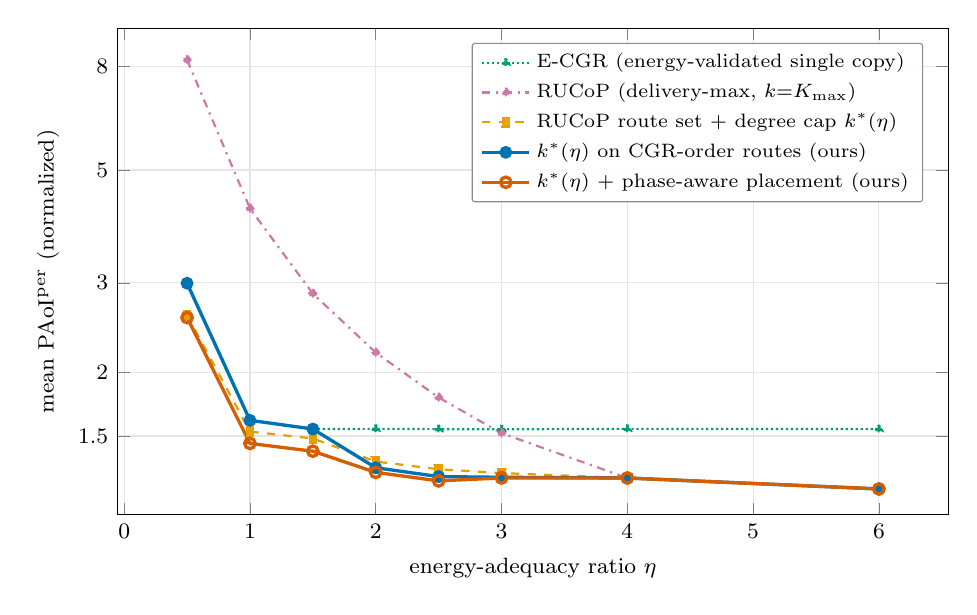
\begin{tikzpicture}
\begin{semilogyaxis}[paperfig,width=\columnwidth,height=0.64\columnwidth,
  xlabel={energy-adequacy ratio $\eta$},ylabel={mean $\PAoIper$ (normalized)},
  legend pos=north east,grid=both,legend cell align=left,
  ymin=1.05,ymax=9.5,ytick={1,1.5,2,3,5,8},
  yticklabels={$1$,$1.5$,$2$,$3$,$5$,$8$},
  error bars/y dir=both,error bars/y explicit]
\addplot[cC,thick,densely dotted,mark=triangle*,mark size=1.5pt] coordinates {(0.5,2.995) +- (0,0.015) (1.0,1.610) +- (0,0.005) (1.5,1.548) +- (0,0.004) (2.0,1.549) +- (0,0.002) (2.5,1.547) +- (0,0.004) (3.0,1.546) +- (0,0.003) (4.0,1.549) +- (0,0.003) (6.0,1.547) +- (0,0.003)};
\addlegendentry{E-CGR (energy-validated single copy)}
\addplot[cD,thick,dashdotted,mark=diamond*,mark size=1.6pt] coordinates {(0.5,8.231) +- (0,0.036) (1.0,4.201) +- (0,0.009) (1.5,2.857) +- (0,0.008) (2.0,2.188) +- (0,0.005) (2.5,1.785) +- (0,0.003) (3.0,1.519) +- (0,0.002) (4.0,1.240) +- (0,0.001) (6.0,1.180) +- (0,0.001)};
\addlegendentry{RUCoP (delivery-max, $k{=}K_{\max}$)}
\addplot[cE,thick,dashed,mark=square*,mark size=1.5pt] coordinates {(0.5,2.593) +- (0,0.012) (1.0,1.530) +- (0,0.003) (1.5,1.483) +- (0,0.001) (2.0,1.336) +- (0,0.002) (2.5,1.290) +- (0,0.001) (3.0,1.268) +- (0,0.001) (4.0,1.240) +- (0,0.001) (6.0,1.180) +- (0,0.001)};
\addlegendentry{RUCoP route set $+$ degree cap $k^\ast(\eta)$}
\addplot[cA,very thick,mark=*,mark size=1.7pt] coordinates {(0.5,2.995) +- (0,0.015) (1.0,1.610) +- (0,0.005) (1.5,1.548) +- (0,0.004) (2.0,1.299) +- (0,0.002) (2.5,1.248) +- (0,0.001) (3.0,1.244) +- (0,0.002) (4.0,1.240) +- (0,0.001) (6.0,1.180) +- (0,0.001)};
\addlegendentry{$k^\ast(\eta)$ on CGR-order routes (ours)}
\addplot[cB,very thick,mark=o,mark size=1.9pt] coordinates {(0.5,2.564) +- (0,0.011) (1.0,1.450) +- (0,0.003) (1.5,1.400) +- (0,0.002) (2.0,1.272) +- (0,0.001) (2.5,1.224) +- (0,0.001) (3.0,1.240) +- (0,0.001) (4.0,1.240) +- (0,0.001) (6.0,1.180) +- (0,0.001)};
\addlegendentry{$k^\ast(\eta)$ $+$ phase-aware placement (ours)}
\end{semilogyaxis}
\end{tikzpicture}
\caption{CGR-family comparison under one budget ($K_{\max}{=}4$
candidate routes with heterogeneous success
$q_i\in\{0.90,0.75,0.60,0.45\}$, ensemble phases, $B{=}12$, ten
seeds, 95\% CIs; logarithmic axis). On this single-hop instance E-CGR
reduces to a reserve-gated single copy on the earliest route and RUCoP
to the most reliable routes (Section~\ref{sec:sim}).}
\label{fig:cgrfamily}
\end{figure}


\paragraph*{Correlated (bursty) route faults}
The i.i.d.\ success model of Proposition~\ref{prop:uncertain} is a
first-order bridge, and experiment E19 tests its mean-level
conclusions when faults are persistent: each route's availability is a
two-state Markov chain with the same stationary $q{=}2/3$ and lag-one
autocorrelation $\rho_1\in\{0,0.5,0.9,0.98\}$ (mean down-dwell $1.5$,
$3$, $15$, and $75$ periods), everything else as in the matched-budget
harness. Mean $\PAoIper$ moves by less than $1.3\%$ across the whole
persistence range at every $(k,\eta)$; a single copy stays $19$--$30\%$
staler than $k^{\ast}$ copies; and the freshness-optimal degree is the
rule's choice at $\eta{=}2$ and $\eta{=}6$ at every persistence. At
$\eta{=}3$ the degrees $k{=}2$ and $k{=}3$ tie within their confidence
intervals at every persistence, including $\rho_1{=}0$
($1.321\pm0.001$ versus $1.320\pm0.002$), and the nominal argmin flips
between them: this is the finite-battery effect of
Section~\ref{sec:r3hard} at $k{=}\eta$ with $B{=}12$, not an effect of
persistence: the exact battery chain for this configuration gives
$1.3212P$ versus $1.3204P$, the simulated tie, so here the rule's choice
is exact only from $B{=}12$, above the $B^{\dagger}(3){=}9$ of the
configuration of Section~\ref{sec:policy}. What persistence changes is the variance: the across-seed
interval of the single-copy mean widens three- to five-fold from
$\rho_1{=}0$ to $0.98$, the same tail effect that bursty harvest has in
E15. For CGR-order placement the i.i.d.\ prediction is the
order-statistic profile \eqref{eq:hord}; it reproduces the simulated
means to within $0.5\%$ up to $\rho_1{=}0.9$ and $1.2\%$ at
$\rho_1{=}0.98$, except in the cells with $k{=}\eta$ exactly, where the
finite battery lowers $\peff$ below its fluid value and the simulation
sits $4\%$ above, which is the work-conservation correction of
Section~\ref{sec:r3hard} (\texttt{e19\_bursty\_faults.py}).

\paragraph*{Reference-implementation cross-check (ION)}
As a final tier we reproduce the Result~1 anchor in ION~4.1.4, the
reference Bundle Protocol implementation~\cite{burleigh2007ion}: two ION
nodes (BPv7, \texttt{ipn} scheme) exchange status bundles over a
contact plan that opens a $W{=}6$\,s window once per $P{=}60$\,s (the
period compressed so that $120$ cycles fit in two hours of wall-clock
time, since ION runs in real time). Over $974$ bundles sent at a
$7.3$\,s cadence (incommensurate with $P$, so arrival phases are
quasi-uniform), delivery is lossless and the delay histogram reproduces
the mixed residual law: an atom near zero plus a uniform slab over the
$54$\,s gap. A per-bundle least-squares regression of the measured
delay on the plan-predicted residual gives slope $1.016$ ($95\%$ CI
$1.013$--$1.019$, $R^2{=}0.998$, $n{=}974$) and intercept
$1.92\pm0.08$\,s. The residual law holds one-for-one per bundle; the
$1.6\%$ excess of the slope over unity is not a departure from it but a
two-population effect. Bundles that arrive inside a window are
dispatched after $0.55$\,s, whereas bundles that waited for a window
pay ION's contact-activation latency of $2.50$\,s (standard deviation
$0.51$\,s, $n{=}879$), and regressing across both populations adds
$0.016$ to the slope (the window-arrival fraction $0.0975$, times the
$1.95$\,s difference of the two lags, times
$\E[R]/\operatorname{Var}R$), which is the measured excess. The
gap-arrival lag is precisely the lumped service
term $T_s$ of the model, here measured in the reference implementation
(the realized-phase residual mean is $24.34$\,s versus the $24.30$\,s
closed form). We stress that this is a reference-implementation cross-check on
a Linux host, not a flight test, and that it says nothing about radio
propagation, interference, or packet loss; its value is that ION has
flight heritage. At operational periods
($P\approx5.7\times10^3$\,s) this $T_s$ is ${\sim}0.04\%$ of the mean:
the gating law, not the software overhead, governs freshness.

\paragraph*{Full heterogeneous end-to-end scenario}
To exercise the complete stack we run the canonical chain sensor $\to$ UAV
mule $\to$ LEO $\to$ gateway in dtnsim, each hop carrying its own contact
model: high-variance (gamma, $\mathrm{CV}{=}1.3$; over-dispersed but
light-tailed) terrestrial gaps, a periodic-with-jitter UAV segment, and a
deterministic LEO segment, with incommensurate cadences. Across ten
seeded replications (each with its own realized contact plan and
per-seed additive prediction $\E[R_1]{+}\E[R_2]{+}\E[R_3]$), the
simulated mean end-to-end delay matches the prediction to within
$5.9\%$ on every seed and to $0.2\%$ in the across-seed mean
($7165$ versus $7176$\,s), supporting the fixed-plan mixing
approximation of Remark~\ref{rem:fixedmix}, and the additive
composition it licenses, across heterogeneous segment types in a
protocol-level CGR stack. For the reference seed, $6754$\,s measured
against $3617{+}758{+}2454{=}6829$\,s predicted over a three-hop path
with $96\%$ delivered and full-chain mean $\OPAoI$
$10.3\times10^{3}$\,s; across the ten seeds the full-chain mean
$\OPAoI$ is $(10.0\pm0.5)\times10^{3}$\,s, i.e.\ $1.75\pm0.08\,P$, the
energy-unconstrained level of Fig.~\ref{fig:hetero}. Adding a finite
battery at the UAV/LEO relays exposes the energy coupling in the
multi-segment setting (Fig.~\ref{fig:hetero}): a relay battery must
cover the per-contact forwarding burst, and below that threshold
end-to-end $\OPAoI$ degrades by an order of magnitude.

% AUTO-GENERATED by figs/make_figures.py -- do not edit.
\begin{figure}[t]\centering
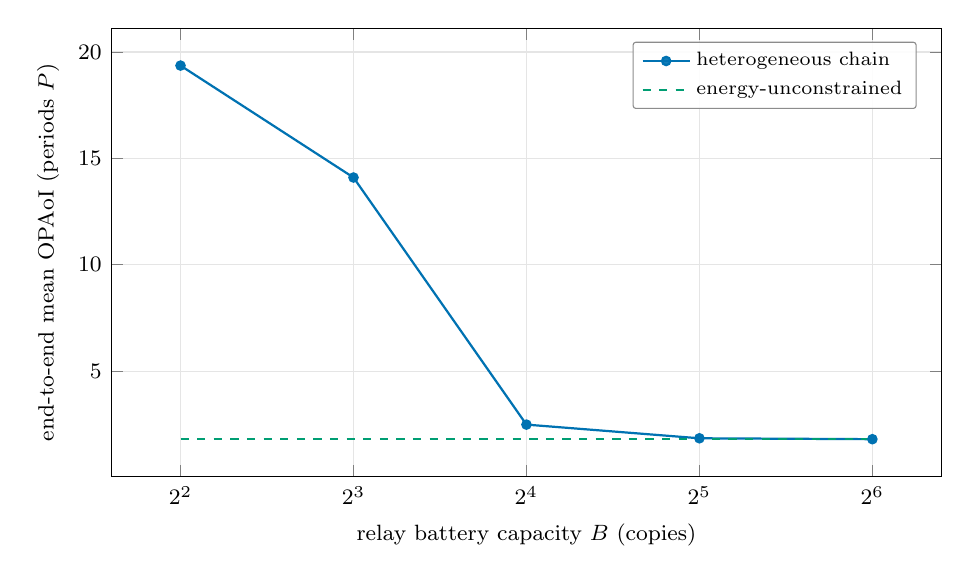
\begin{tikzpicture}
\begin{axis}[paperfig,width=\columnwidth,height=0.6\columnwidth,
  xlabel={relay battery capacity $B$ (copies)},
  ylabel={end-to-end mean OPAoI (periods $P$)},grid=both,
  xmode=log,log basis x=2,legend pos=north east,legend cell align=left]
\addplot[cA,thick,mark=*,mark size=1.5pt] coordinates {(4.0,19.361) (8.0,14.100) (16.0,2.487) (32.0,1.844) (64.0,1.802)};
\addlegendentry{heterogeneous chain}
\addplot[cC,thick,dashed,no marks] coordinates {(4,1.802) (64,1.802)};
\addlegendentry{energy-unconstrained}
\end{axis}
\end{tikzpicture}
\caption{Energy coupling in the full heterogeneous chain (sensor $\to$ UAV
mule $\to$ LEO $\to$ gateway, dtnsim CGR, reference seed). A finite
battery at the UAV and LEO relays must cover the per-contact forwarding
burst; below that size end-to-end mean OPAoI degrades by about
$11\times$ and delivery falls from $96\%$ to $31\%$. With a sufficient
battery the chain matches its energy-unconstrained level.}
\label{fig:hetero}
\end{figure}


\paragraph*{Order preservation on the chain}
The per-update identity presumes order-preserving deliveries
(Section~\ref{sec:model}). Experiment E20 measures the inversion
frequency on S3 by model-exact simulation of its three gated
first-in-first-out (FIFO) segments, at the Tier-2 cadence ($400$\,s; latency spread up to $117$
generation intervals) and at one update per LEO period: in ten seeds
(about $5.5\times10^{3}$ and $380$ updates each) \emph{no} delivery arrives
stale, and the per-update peak evaluated on the resetting subsequence
equals $\E[Z]+\E[Y]$ to $0.03\%$. The reason is structural and worth
stating. On a single path whose segments forward in FIFO order,
departures from every segment preserve arrival order, so generation
order is preserved end to end regardless of the latency spread; and an
earliest-arrival router over a shared plan preserves it too, since the
earlier update could have taken the later update's route. Inversions
therefore require consecutive updates to take different routes under
\emph{changing} conditions (re-routing after a fault, or copies over
distinct routes), which is exactly where our Tier-2 reconstruction
counts only freshness-resetting deliveries and the identity is not
relied upon.

\paragraph*{Where the low-load regime ends}
The uncongested-contact scope of Section~\ref{sec:model} is quantified
by loading contacts to capacity: we fix the window's carrying capacity
at $M{=}8$ bundles (contact rate set so a $430$\,s window serializes and
volume-books exactly $M$; CGR is volume-aware), with $M{=}64$ as the
unloaded control on the same seeds, and sweep the offered update rate
from ${\sim}1$ to $16$ per period at $k{=}1$ (single relay) and $k{=}2$
(three-relay staggered diamond, where each relay window carries about
two thirds of the copies). The experiment has three seeds, so we report
per-seed ratios of loaded to unloaded mean delay rather than intervals.
With $\rho_{\mathrm{load}}$ the offered copies per window divided by
$M$, the single-copy ratios are $1.00$--$1.03$ up to
$\rho_{\mathrm{load}}{=}0.5$ (one seed at $1.12$ at the lowest load),
$1.05$--$1.38$ at $\rho_{\mathrm{load}}{=}1$, where paced arrivals are
still stable, and $117$--$124$ at $\rho_{\mathrm{load}}{=}2$, where the
delivered fraction drops to the capacity ratio. Below capacity OPAoI
keeps \emph{improving} with offered load, as more updates ride each
window. The failure is thus a step of two orders of magnitude, not a
knee, and no hypothesis test is needed to locate it; inside the
boundary the low-load model holds to within a few percent, loosening to
tens of percent in the worst seed exactly at capacity. Replication
multiplies the offered contact volume by the copy count: the two-copy
run is only mildly affected at $8$ updates per period
($\rho_{\mathrm{load}}{=}0.67$, ratios $1.05$--$1.13$) and past the wall
at $16$ ($\rho_{\mathrm{load}}{=}1.33$, ratios $95$--$101$). The
boundary of validity is thus predictable (offered copies per window
below $M$), and inside it the freshness analysis stands; beyond it,
contact-volume management (overbooking,
CGR-ETO~\cite{bezirgiannidis}), not freshness-optimal replication, is
the binding problem. This test sweeps one parameter on
single-relay and three-relay plans; on a multi-hop path the same step
occurs at the most loaded contact, but we have not measured how the
boundary moves with hop count.

\paragraph*{Scope and limitations}
The results above hold under assumptions that we collect here (see also
Table~\ref{tab:assumptions}). \emph{Uncongested contacts:} every
freshness law and policy statement in this paper presumes offered
copies per window below the window's capacity; once a real network
approaches contact capacity, as loaded satellite links can, the
gating-driven freshness analysis is replaced by the contact-volume
problem above. \emph{Fixed cadence:} the threshold assumes application-paced
sampling; a source that can sample at will and whose routes diverge at
the source should place a fresh sample on each route instead
(Section~\ref{sec:model}). \emph{Single energy bottleneck:} one battery gates copy
launches; real DTNs have a battery at every relay, and the
heterogeneous-chain experiment shows that relay batteries matter
(Fig.~\ref{fig:hetero}) without being modeled by the threshold.
\emph{Battery size and estimators:} the two-candidate rule is the
large-battery rule; below the computable size $B^{\dagger}(\eta)$ the
chain-evaluated objective is needed (Section~\ref{sec:policy}), and the
estimators $\hat\eta$ and $\hat q$ are proposed but not evaluated.
\emph{Validation depth differs by tier:} every analytical claim is
checked model-exactly, but Tier~2 corroborates a subset (residual laws,
composition, the starvation side of the threshold, the capacity
boundary) and ION only the residual-wait anchor. The hedging benefit of
replication is computed model-exactly as a function of the per-pass
route success $q$; which $q$ a deployment realizes depends on whether
its faults destroy bundles or merely delay them, and under dtnsim's
stall-type faults, which CGR routes around, the hedge is within seed
noise or absent. The tail corollary is
likewise validated model-exactly only, because we did not export
per-update peak distributions from the Tier-2 runs. \emph{Constellation:} the
ephemeris results use Iridium-NEXT; the laws depend on a constellation
only through $(P,W)$, the revisit pattern, and the pair-phase
structure, so other LEO shells change the numbers (periods of
$90$--$130$\,min, multiple passes per period for dense shells, for
which the renewal law with random gaps applies) but not the structure,
and the ladder bounds \eqref{eq:ladder} are constellation-independent.
\emph{Segment models:} the UAV and terrestrial segments are abstract
renewal models, not trajectories; linking them to specific UAV
trajectories or terrestrial mobility traces is future work.


% =====================================================================
\FloatBarrier
\section{Conclusion}
We studied information freshness over scheduled, intermittently
connected multi-segment DTNs with energy-constrained bundle
replication. One alternating-renewal model yields the residual-wait
laws for LEO, UAV, and terrestrial segments and the exact inversion
condition \eqref{eq:invcond} under which peak age falls below average
age; phase mixing (exact under random offsets, measured on fixed
plans) makes end-to-end latency compose, with the two-copy gain equal
to half the mean absolute difference of path latencies. For the periodic
gating bottleneck, a large battery, and the fixed-cadence,
all-or-nothing policy family, the energy budget admits a
near-threshold optimal degree
($\lfloor\lambda_e P/e\rfloor$ or the skip-aware neighbor, capped at
$K_{\max}$; monotone and saturating; rules that fire a partial degree
do up to $2.7\%$ better where energy is not scarce), extended by
Proposition~\ref{prop:uncertain} to per-copy route success $q$. Route
uncertainty, the true source of the replication gain, thus enters the
same objective, and replication under uncertainty buys \emph{cadence}
as well as latency spread. The floor/ceiling structure is
proved below the floor and holds beyond it under an explicit,
grid-verified increment condition; a finite battery exerts downward
pressure on the optimum, and the battery size from which the
two-candidate rule is exact is computable from the stationary battery
chain.

All analytical results are validated under their stated assumptions by
model-exact Monte Carlo. Representative results (the residual laws,
the additive composition, the atomic starvation penalty, and the
capacity boundary) are corroborated in a DTN-realistic BP/CGR
simulator, and the residual-wait anchor is independently
reproduced in the ION reference implementation (lossless delivery, the
law exact per bundle, and the dispatch overhead measurable as the
model's $T_s$). The hedging benefit of replication is computed
model-exactly as a function of the per-pass route success (a single
copy is $19$--$30\%$ staler when each route succeeds with probability
two thirds). In the DTN stack the over-replication penalty is
corroborated, while under stall-type faults that CGR routes around the
hedge is within seed noise or absent; how much replication buys in a
deployment therefore depends on whether its faults destroy bundles or
merely delay them. The degree rule survives bursty
(Markov-modulated) harvest up to a mean dwell of ten contact periods and
holds or ties under bursty route faults at every tested persistence.
Real Iridium-NEXT ephemeris confirms the residual law on a reference
satellite and the pair-phase dependence of the route-set
latency-diversity potential; on a synthetic heterogeneous-route
instance, a per-bundle \emph{phase-aware placement} rule is best or
tied for best at every energy level. The framework extends, rather than
replaces, the CGR/RUCoP contact-plan stack: on that instance the degree
rule matches an E-CGR-style energy-validated single copy where energy
affords one copy and improves on it beyond, and RUCoP's route set under
the degree cap recovers most of what energy-blind replication loses.
Two limitations govern deployment. All results presume the
uncongested-contact regime, with offered copies below contact
capacity, and are replaced by contact-volume management beyond it;
and the single-bottleneck energy model leaves per-relay batteries to
future work. Where contact prediction is accurate and relays reliable,
the replication gain shrinks toward the oracle tie; the rule follows it
only if its objective uses the gain profile of the placement in use.
Ongoing work treats regime-aware degree adaptation under strongly
persistent harvest (beyond the measured dwell-$20$ boundary),
Markov-modulated contact schedules beyond the renewal assumption, and
per-relay energy budgets.

% =====================================================================
\section*{Data availability}
Code, contact-plan scenarios, all result data (CSV), and the scripts
that regenerate every figure are publicly available at
\url{https://github.com/UNO-Networks-Lab/paoi-scheduled-dtn} (MIT license) and
archived on Zenodo (doi:\allowbreak
\url{10.5281/zenodo.21841317}). The repository includes a README with
installation and environment-setup instructions, the command that
reproduces each experiment and figure, the seed sets, a frozen copy of
the reported dataset with a comparison script, and the experiment-to-claim
validation matrix; the project page mirrors the manuscript.

\section*{CRediT authorship contribution statement}
\textbf{Haoyu Wang}: Conceptualization, Methodology, Software, Formal
analysis, Investigation, Validation, Data curation, Visualization,
Writing -- original draft, Writing -- review \& editing.
\textbf{Bo Sheng}: Conceptualization, Methodology, Supervision,
Validation, Writing -- review \& editing.
\textbf{Xiaoqian Zhang}: Conceptualization, Methodology, Supervision,
Project administration, Writing -- review \& editing, Funding
acquisition.

\section*{Funding}
This work was supported in part by the U.S. National Science Foundation
(NSF) under Award No.~2450832 and by the Nebraska Research Initiative.

\section*{Declaration of competing interest}
The authors declare that they have no known competing financial
interests or personal relationships that could have appeared to
influence the work reported in this paper. The Iridium-NEXT ephemeris
used is public two-line-element data from CelesTrak; no proprietary
operator data were used, and the authors have no relationship with any
satellite operator.

\section*{Declaration of generative AI and AI-assisted technologies
in the writing process}
During the preparation of this work, the authors used generative AI
tools (ChatGPT and Claude) to assist with language refinement,
manuscript organization, and literature cross-checking. These tools
were not used to produce the content of the paper, such as the model,
the mathematical proofs, or the experimental results. After using
these tools, the authors reviewed and edited the content as needed
and take full responsibility for the content of the published article.

\balance
\begin{thebibliography}{99}
% Elsevier numbered style (DCN guide for authors), in order of first citation.
\bibitem{jiang2023sdn}
W.~Jiang, Software defined satellite networks: a survey, Digit. Commun. Netw. 9~(6) (2023) 1243--1264.
\bibitem{ullah2025mgmt}
I.~Ullah, A.~Arishi, S.K.~Singh, F.~Alharbi, A.H.~Ibrahim, M.~Islam, Y.I.~Daradkeh, C.~Choi, Autonomous network management for 6G communication: a comprehensive survey, Digit. Commun. Netw. 11~(6) (2025) 1917--1940.
\bibitem{he2026wass}
Y.~He, L.~Hu, L.~Chen, Wasserstein distance-based interference characterization and analysis in NGSO constellations with non-homogeneous stochastic geometry, Digit. Commun. Netw. 12~(7) (2026) 1116--1125.
\bibitem{he2026ngso}
Y.~He, C.~Qi, D.~Yan, A geometric relationship-aware and real-time coverage analysis for mega NGSO satellite constellations, Digit. Commun. Netw. 12~(10) (2026) 1656--1668.
\bibitem{rucop}
F.D.~Raverta, J.A.~Fraire, P.G.~Madoery, R.A.~Demasi, J.M.~Finochietto, P.R.~D'Argenio, Routing in delay-tolerant networks under uncertain contact plans, Ad Hoc Netw. 123 (2021) 102663.
\bibitem{ari}
{\c C}.~Ar{\i}, \"O.T.~Kartal, A.~Munari, L.~Badia, E.~Uysal, O.~Kaya, Optimizing peak age under intermittent satellite connectivity and store-and-forward, in: Proc. 59th Asilomar Conf. Signals, Systems, and Computers, 2025, pp.~140--144.
\bibitem{atasayar2025}
A.U.~Atasayar, A.~Li, {\c C}.~Ar{\i}, E.~Uysal, Age optimal sampling and routing under intermittent links and energy constraints, arXiv preprint arXiv:2512.00985 (2025). \url{https://doi.org/10.48550/arXiv.2512.00985}; conference version: Fresh data delivery: joint sampling and routing for minimizing the age of information, in: Proc. ACM MobiHoc, 2025, pp.~291--300. \url{https://doi.org/10.1145/3704413.3764413}.
\bibitem{zhao2026aoi}
F.~Zhao, N.~Pappas, S.~Jin, H.H.~Yang, Age of information in non-terrestrial networks with energy harvesting, arXiv preprint arXiv:2608.02485 (2026), submitted for publication. \url{https://doi.org/10.48550/arXiv.2608.02485}.
\bibitem{badia2025globecom}
L.~Badia, A.~Munari, Delay tolerant networking helps reducing age of information under intermittent connectivity, in: Proc. IEEE Globecom Workshops (GC Wkshps), 2025, pp.~1059--1064.
\bibitem{kaul2012}
S.K.~Kaul, R.D.~Yates, M.~Gruteser, Real-time status: how often should one update?, in: Proc. IEEE INFOCOM, 2012, pp.~2731--2735.
\bibitem{costa2016}
M.~Costa, M.~Codreanu, A.~Ephremides, On the age of information in status update systems with packet management, IEEE Trans. Inf. Theory 62~(4) (2016) 1897--1910.
\bibitem{yates2021survey}
R.D.~Yates, Y.~Sun, D.R.~Brown, S.K.~Kaul, E.~Modiano, S.~Ulukus, Age of information: an introduction and survey, IEEE J. Sel. Areas Commun. 39~(5) (2021) 1183--1210.
\bibitem{kosta2017}
A.~Kosta, N.~Pappas, V.~Angelakis, Age of information: a new concept, metric, and tool, Found. Trends Netw. 12~(3) (2017) 162--259.
\bibitem{wu2026xoi}
B.~Wu, J.~Huang, S.~Yu, ``X of information'' continuum: a survey on AI-driven multi-dimensional metrics for next-generation networked systems, IEEE Commun. Surv. Tutor. 28 (2026) 5307--5344.
\bibitem{huang2015}
L.~Huang, E.~Modiano, Optimizing age-of-information in a multi-class queueing system, in: Proc. IEEE Int. Symp. Inf. Theory (ISIT), 2015, pp.~1681--1685.
\bibitem{champati2019}
J.P.~Champati, H.~Al-Zubaidy, J.~Gross, On the distribution of AoI for the GI/GI/1/1 and GI/GI/1/2* systems: exact expressions and bounds, in: Proc. IEEE INFOCOM, 2019, pp.~37--45.
\bibitem{bedewy2017}
A.M.~Bedewy, Y.~Sun, N.B.~Shroff, Age-optimal information updates in multihop networks, in: Proc. IEEE Int. Symp. Inf. Theory (ISIT), 2017, pp.~576--580.
\bibitem{bedewy2019}
A.M.~Bedewy, Y.~Sun, N.B.~Shroff, The age of information in multihop networks, IEEE/ACM Trans. Netw. 27~(3) (2019) 1248--1257.
\bibitem{yates2020}
R.D.~Yates, The age of information in networks: moments, distributions, and sampling, IEEE Trans. Inf. Theory 66~(9) (2020) 5712--5728.
\bibitem{talak2018}
R.~Talak, S.~Karaman, E.~Modiano, Optimizing information freshness in wireless networks under general interference constraints, in: Proc. ACM MobiHoc, 2018, pp.~61--70.
\bibitem{kam2016}
C.~Kam, S.~Kompella, G.D.~Nguyen, A.~Ephremides, Effect of message transmission path diversity on status age, IEEE Trans. Inf. Theory 62~(3) (2016) 1360--1374.
\bibitem{sinha}
A.~Sinha, S.~Singhvi, P.D.~Mankar, H.S.~Dhillon, Peak age of information under tandem of queues, in: Proc. IEEE Int. Symp. Inf. Theory (ISIT), 2024, pp.~951--956.
\bibitem{senthilkumar}
M.S.~Kumar, A.~Dadlani, H.~Tabassum, Age of information in unreliable tandem queues, IEEE Commun. Lett. 29~(10) (2025) 2308--2312.
\bibitem{parag2017}
P.~Parag, A.~Taghavi, J.-F.~Chamberland, On real-time status updates over symbol erasure channels, in: Proc. IEEE Wireless Commun. Netw. Conf. (WCNC), 2017, pp.~1--6.
\bibitem{najm2019}
E.~Najm, E.~Telatar, R.~Nasser, Optimal age over erasure channels, in: Proc. IEEE Int. Symp. Inf. Theory (ISIT), 2019, pp.~335--339.
\bibitem{devassy2019}
R.~Devassy, G.~Durisi, G.C.~Ferrante, O.~Simeone, E.~Uysal, Reliable transmission of short packets through queues and noisy channels under latency and peak-age violation guarantees, IEEE J. Sel. Areas Commun. 37~(4) (2019) 721--734.
\bibitem{chen2022}
X.~Chen, K.~Gatsis, H.~Hassani, S.S.~Bidokhti, Age of information in random access channels, IEEE Trans. Inf. Theory 68~(10) (2022) 6548--6568.
\bibitem{chiariotti}
F.~Chiariotti, O.~Vikhrova, B.~Soret, P.~Popovski, Age of information in multihop connections with tributary traffic and no preemption, IEEE Trans. Commun. 70~(10) (2022) 6718--6733; LEO multi-hop analysis in the companion preprint: Information freshness of updates sent over LEO satellite multi-hop networks, arXiv preprint arXiv:2007.05449 (2020), \url{https://doi.org/10.48550/arXiv.2007.05449}.
\bibitem{bacinoglu2015}
B.T.~Bacinoglu, E.T.~Ceran, E.~Uysal-Biyikoglu, Age of information under energy replenishment constraints, in: Proc. Inf. Theory Appl. Workshop (ITA), 2015, pp.~25--31.
\bibitem{wu2018}
X.~Wu, J.~Yang, J.~Wu, Optimal status update for age of information minimization with an energy harvesting source, IEEE Trans. Green Commun. Netw. 2~(1) (2018) 193--204.
\bibitem{arafa2020}
A.~Arafa, J.~Yang, S.~Ulukus, H.V.~Poor, Age-minimal transmission for energy harvesting sensors with finite batteries: online policies, IEEE Trans. Inf. Theory 66~(1) (2020) 534--556.
\bibitem{bacinoglu2018}
B.T.~Bacinoglu, Y.~Sun, E.~Uysal-Biyikoglu, V.~Mutlu, Achieving the age-energy tradeoff with a finite-battery energy harvesting source, in: Proc. IEEE Int. Symp. Inf. Theory (ISIT), 2018, pp.~876--880.
\bibitem{sun2017}
Y.~Sun, E.~Uysal-Biyikoglu, R.D.~Yates, C.E.~Koksal, N.B.~Shroff, Update or wait: how to keep your data fresh, IEEE Trans. Inf. Theory 63~(11) (2017) 7492--7508.
\bibitem{ceran2019}
E.T.~Ceran, D.~G\"und\"uz, A.~Gy\"orgy, Reinforcement learning to minimize age of information with an energy harvesting sensor with HARQ and sensing cost, in: Proc. IEEE INFOCOM Workshops, 2019, pp.~656--661.
\bibitem{fall2003}
K.~Fall, A delay-tolerant network architecture for challenged internets, in: Proc. ACM SIGCOMM, 2003, pp.~27--34.
\bibitem{rfc4838}
V.~Cerf, S.~Burleigh, A.~Hooke, L.~Torgerson, R.~Durst, K.~Scott, K.~Fall, H.~Weiss, Delay-tolerant networking architecture, RFC 4838, Internet Research Task Force (IRTF), 2007.
\bibitem{rfc5050}
K.~Scott, S.~Burleigh, Bundle protocol specification, RFC 5050, Internet Research Task Force (IRTF), 2007.
\bibitem{rfc9171}
S.~Burleigh, K.~Fall, E.J.~Birrane, Bundle protocol version 7, RFC 9171, Internet Engineering Task Force, 2022.
\bibitem{araniti2015}
G.~Araniti, N.~Bezirgiannidis, E.~Birrane, I.~Bisio, S.~Burleigh, C.~Caini, M.~Feldmann, M.~Marchese, J.~Segui, K.~Suzuki, Contact graph routing in DTN space networks: overview, enhancements and performance, IEEE Commun. Mag. 53~(3) (2015) 38--46.
\bibitem{burleigh2007ion}
S.~Burleigh, Interplanetary overlay network: an implementation of the DTN bundle protocol, in: Proc. IEEE Consumer Commun. Netw. Conf. (CCNC), 2007, pp.~222--226.
\bibitem{fraire2015cpd}
J.A.~Fraire, J.M.~Finochietto, Design challenges in contact plans for disruption-tolerant satellite networks, IEEE Commun. Mag. 53~(5) (2015) 163--169.
\bibitem{madoery2016}
J.A.~Fraire, P.G.~Madoery, J.M.~Finochietto, Traffic-aware contact plan design for disruption-tolerant space sensor networks, Ad Hoc Netw. 47 (2016) 41--52.
\bibitem{fraire2017}
J.A.~Fraire, P.~Madoery, S.~Burleigh, M.~Feldmann, J.~Finochietto, A.~Charif, N.~Zergainoh, R.~Velazco, Assessing contact graph routing performance and reliability in distributed satellite constellations, J. Comput. Netw. Commun. 2017 (2017) 2830542.
\bibitem{bezirgiannidis}
N.~Bezirgiannidis, C.~Caini, V.~Tsaoussidis, Analysis of contact graph routing enhancements for DTN space communications, Int. J. Satell. Commun. Netw. 34~(5) (2016) 695--709.
\bibitem{ecgr}
M.~Marchese, F.~Patrone, E-CGR: energy-aware contact graph routing over nanosatellite networks, IEEE Trans. Green Commun. Netw. 4~(3) (2020) 890--902.
\bibitem{wang3dehr}
J.~Wang, R.~Zhang, J.~Yuan, X.~Du, A 3-D energy-harvesting-aware routing scheme for space nanosatellite networks, IEEE Internet Things J. 5~(4) (2018) 2729--2740.
\bibitem{vahdat2000}
A.~Vahdat, D.~Becker, Epidemic routing for partially connected ad hoc networks, Tech. Rep. CS-2000-06, Department of Computer Science, Duke University, Durham, NC, 2000.
\bibitem{spyropoulos2005}
T.~Spyropoulos, K.~Psounis, C.S.~Raghavendra, Spray and wait: an efficient routing scheme for intermittently connected mobile networks, in: Proc. ACM SIGCOMM Workshop on Delay-Tolerant Networking (WDTN), 2005, pp.~252--259.
\bibitem{lindgren2003}
A.~Lindgren, A.~Doria, O.~Schel\'en, Probabilistic routing in intermittently connected networks, ACM SIGMOBILE Mob. Comput. Commun. Rev. 7~(3) (2003) 19--20.
\bibitem{azari2022}
M.M.~Azari, S.~Solanki, S.~Chatzinotas, O.~Kodheli, H.~Sallouha, A.~Colpaert, J.F.~Mendoza Montoya, S.~Pollin, A.~Haqiqatnejad, A.~Mostaani, E.~Lagunas, B.~Ottersten, Evolution of non-terrestrial networks from 5G to 6G: a survey, IEEE Commun. Surv. Tutor. 24~(4) (2022) 2633--2672.
\bibitem{giordani2021}
M.~Giordani, M.~Zorzi, Non-terrestrial networks in the 6G era: challenges and opportunities, IEEE Netw. 35~(2) (2021) 244--251.
\bibitem{liu2018sagin}
J.~Liu, Y.~Shi, Z.M.~Fadlullah, N.~Kato, Space-air-ground integrated network: a survey, IEEE Commun. Surv. Tutor. 20~(4) (2018) 2714--2741.
\bibitem{zhao2004ferry}
W.~Zhao, M.~Ammar, E.~Zegura, A message ferrying approach for data delivery in sparse mobile ad hoc networks, in: Proc. ACM MobiHoc, 2004, pp.~187--198.
\bibitem{shah2003mules}
R.C.~Shah, S.~Roy, S.~Jain, W.~Brunette, Data MULEs: modeling a three-tier architecture for sparse sensor networks, in: Proc. IEEE Workshop Sensor Netw. Protocols Appl. (SNPA), 2003, pp.~30--41.
\bibitem{huang2025uav}
J.~Huang, B.~Wu, Q.~Duan, L.~Dong, S.~Yu, A fast UAV trajectory planning framework in RIS-assisted communication systems with accelerated learning via multithreading and federating, IEEE Trans. Mob. Comput. 24~(8) (2025) 6870--6885.
\bibitem{zhou2026uavai}
L.~Zhou, H.~Yin, H.~Zhao, J.~Wei, D.~Hu, V.C.M.~Leung, A comprehensive survey of artificial intelligence applications in UAV-enabled wireless networks, Digit. Commun. Netw. 12~(4) (2026) 561--583.
\bibitem{abdelmagid2019}
M.A.~Abd-Elmagid, H.S.~Dhillon, Average peak age-of-information minimization in UAV-assisted IoT networks, IEEE Trans. Veh. Technol. 68~(2) (2019) 2003--2008.
\bibitem{isayama}
F.~Isayama, T.~Shigeyasu, A study on DTN routing protocol for disaster situation while considering age of information, Internet Things 34 (2025) 101756.
\bibitem{e3f}
V.S.H.~Huynh, M.~Radenkovic, A novel cross-layer framework for large scale emergency communications, in: Proc. Int. Wireless Commun. Mobile Comput. Conf. (IWCMC), 2017, pp.~2152--2157.
\bibitem{badia2025}
L.~Badia, A.~Munari, Satellite intermittent connectivity and its impact on age of information for finite horizon scheduling, in: Proc. Adv. Satell. Multimedia Syst. Conf. and Signal Process. Space Commun. Workshop (ASMS/SPSC), 2025, pp.~1--8.
\bibitem{delfani2025}
E.~Delfani, N.~Pappas, Semantics-aware updates from remote energy harvesting devices to interconnected LEO satellites, IEEE Commun. Lett. 29~(8) (2025) 1928--1932.
\bibitem{kuipers1974}
L.~Kuipers, H.~Niederreiter, Uniform Distribution of Sequences, Wiley, New York, 1974.
\bibitem{fraire2017dtnsim}
J.A.~Fraire, P.~Madoery, F.~Raverta, J.M.~Finochietto, R.~Velazco, DtnSim: bridging the gap between simulation and implementation of space-terrestrial DTNs, in: Proc. 6th Int. Conf. Space Mission Challenges for Information Technology (SMC-IT), 2017, pp.~120--123.
\bibitem{ma2026igso}
C.~Ma, Z.~Chen, Y.~Zhan, Y.~Su, S.~Jin, G.~Li, L.~Yin, IGSO constellation based polar satellite communication: system design, performance analysis, and LLM-based adaptive transmission, Digit. Commun. Netw. 12~(10) (2026) 1563--1575.
\end{thebibliography}

\end{document}
